\chapter[strategy][strategy]{$\Htautau$ analysis strategy}
\label{chap:strategy}

\begin{quote}
The strategy of the $\Htautau$ strategy is described.
\end{quote}

\section{Introduction}
\label{sec:strategy-introduction}

\section{Categorization}
\label{sec:strategy-categorization}

\begin{figure}[tp]
  \centering
  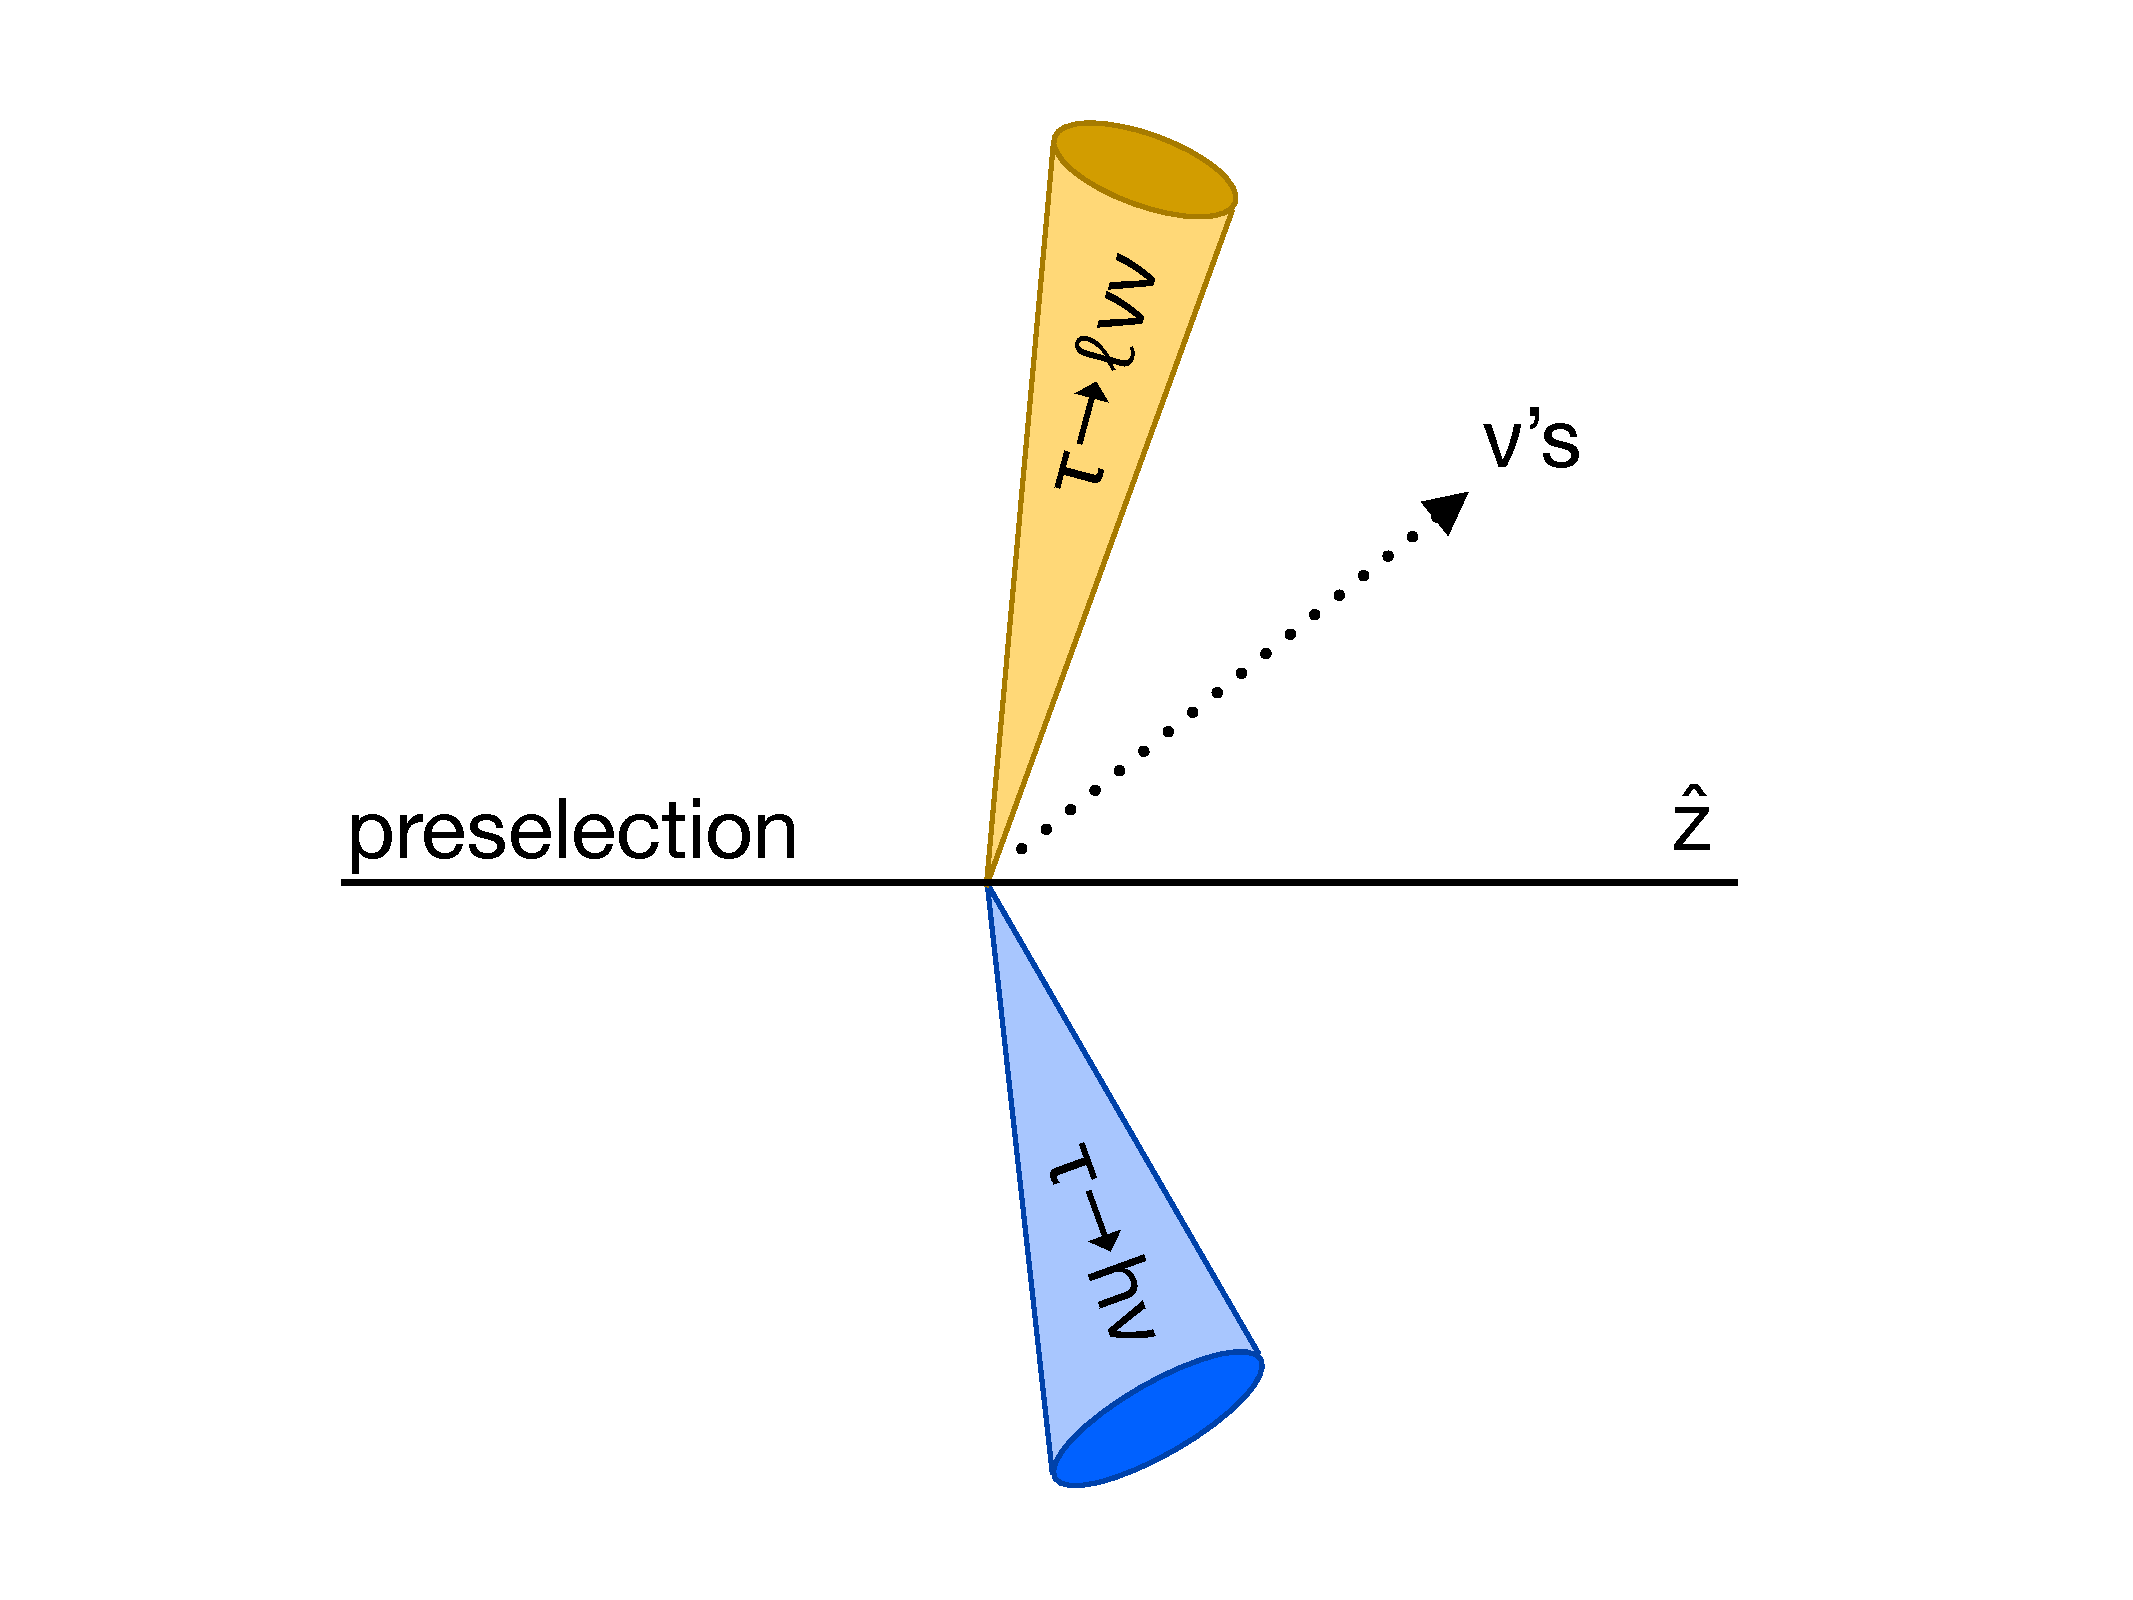
\includegraphics[width=0.48\textwidth]{figures/category-cartoons/presel}
  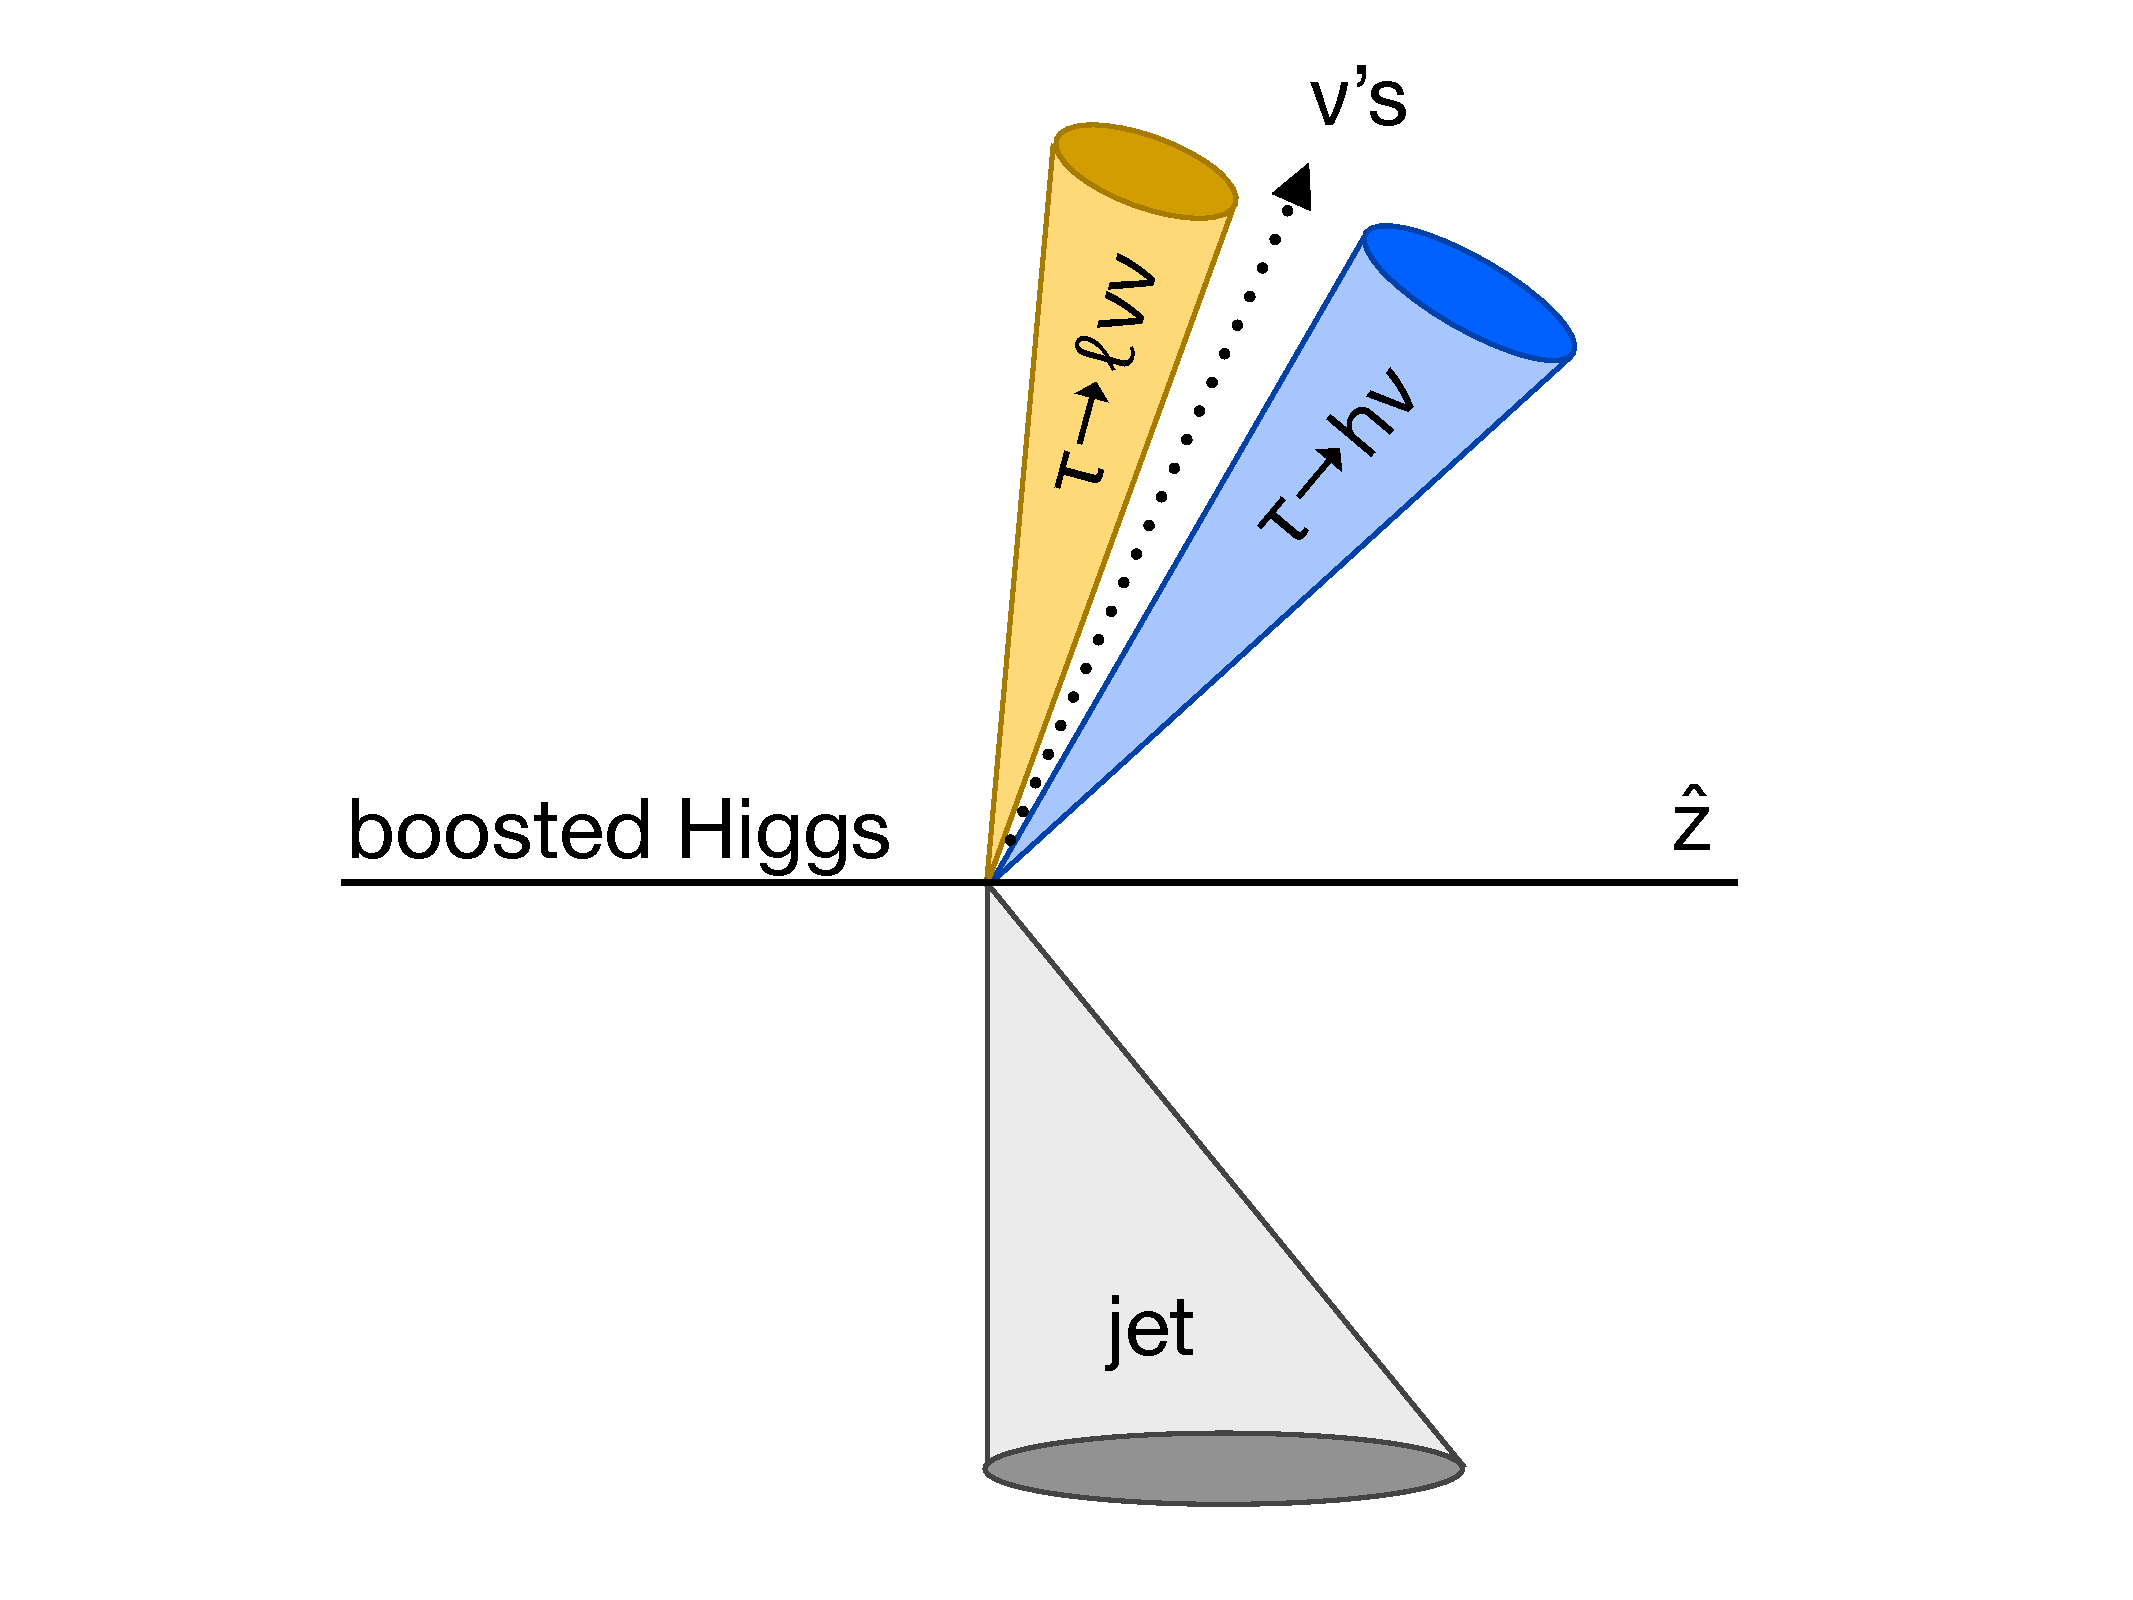
\includegraphics[width=0.48\textwidth]{figures/category-cartoons/boost}
  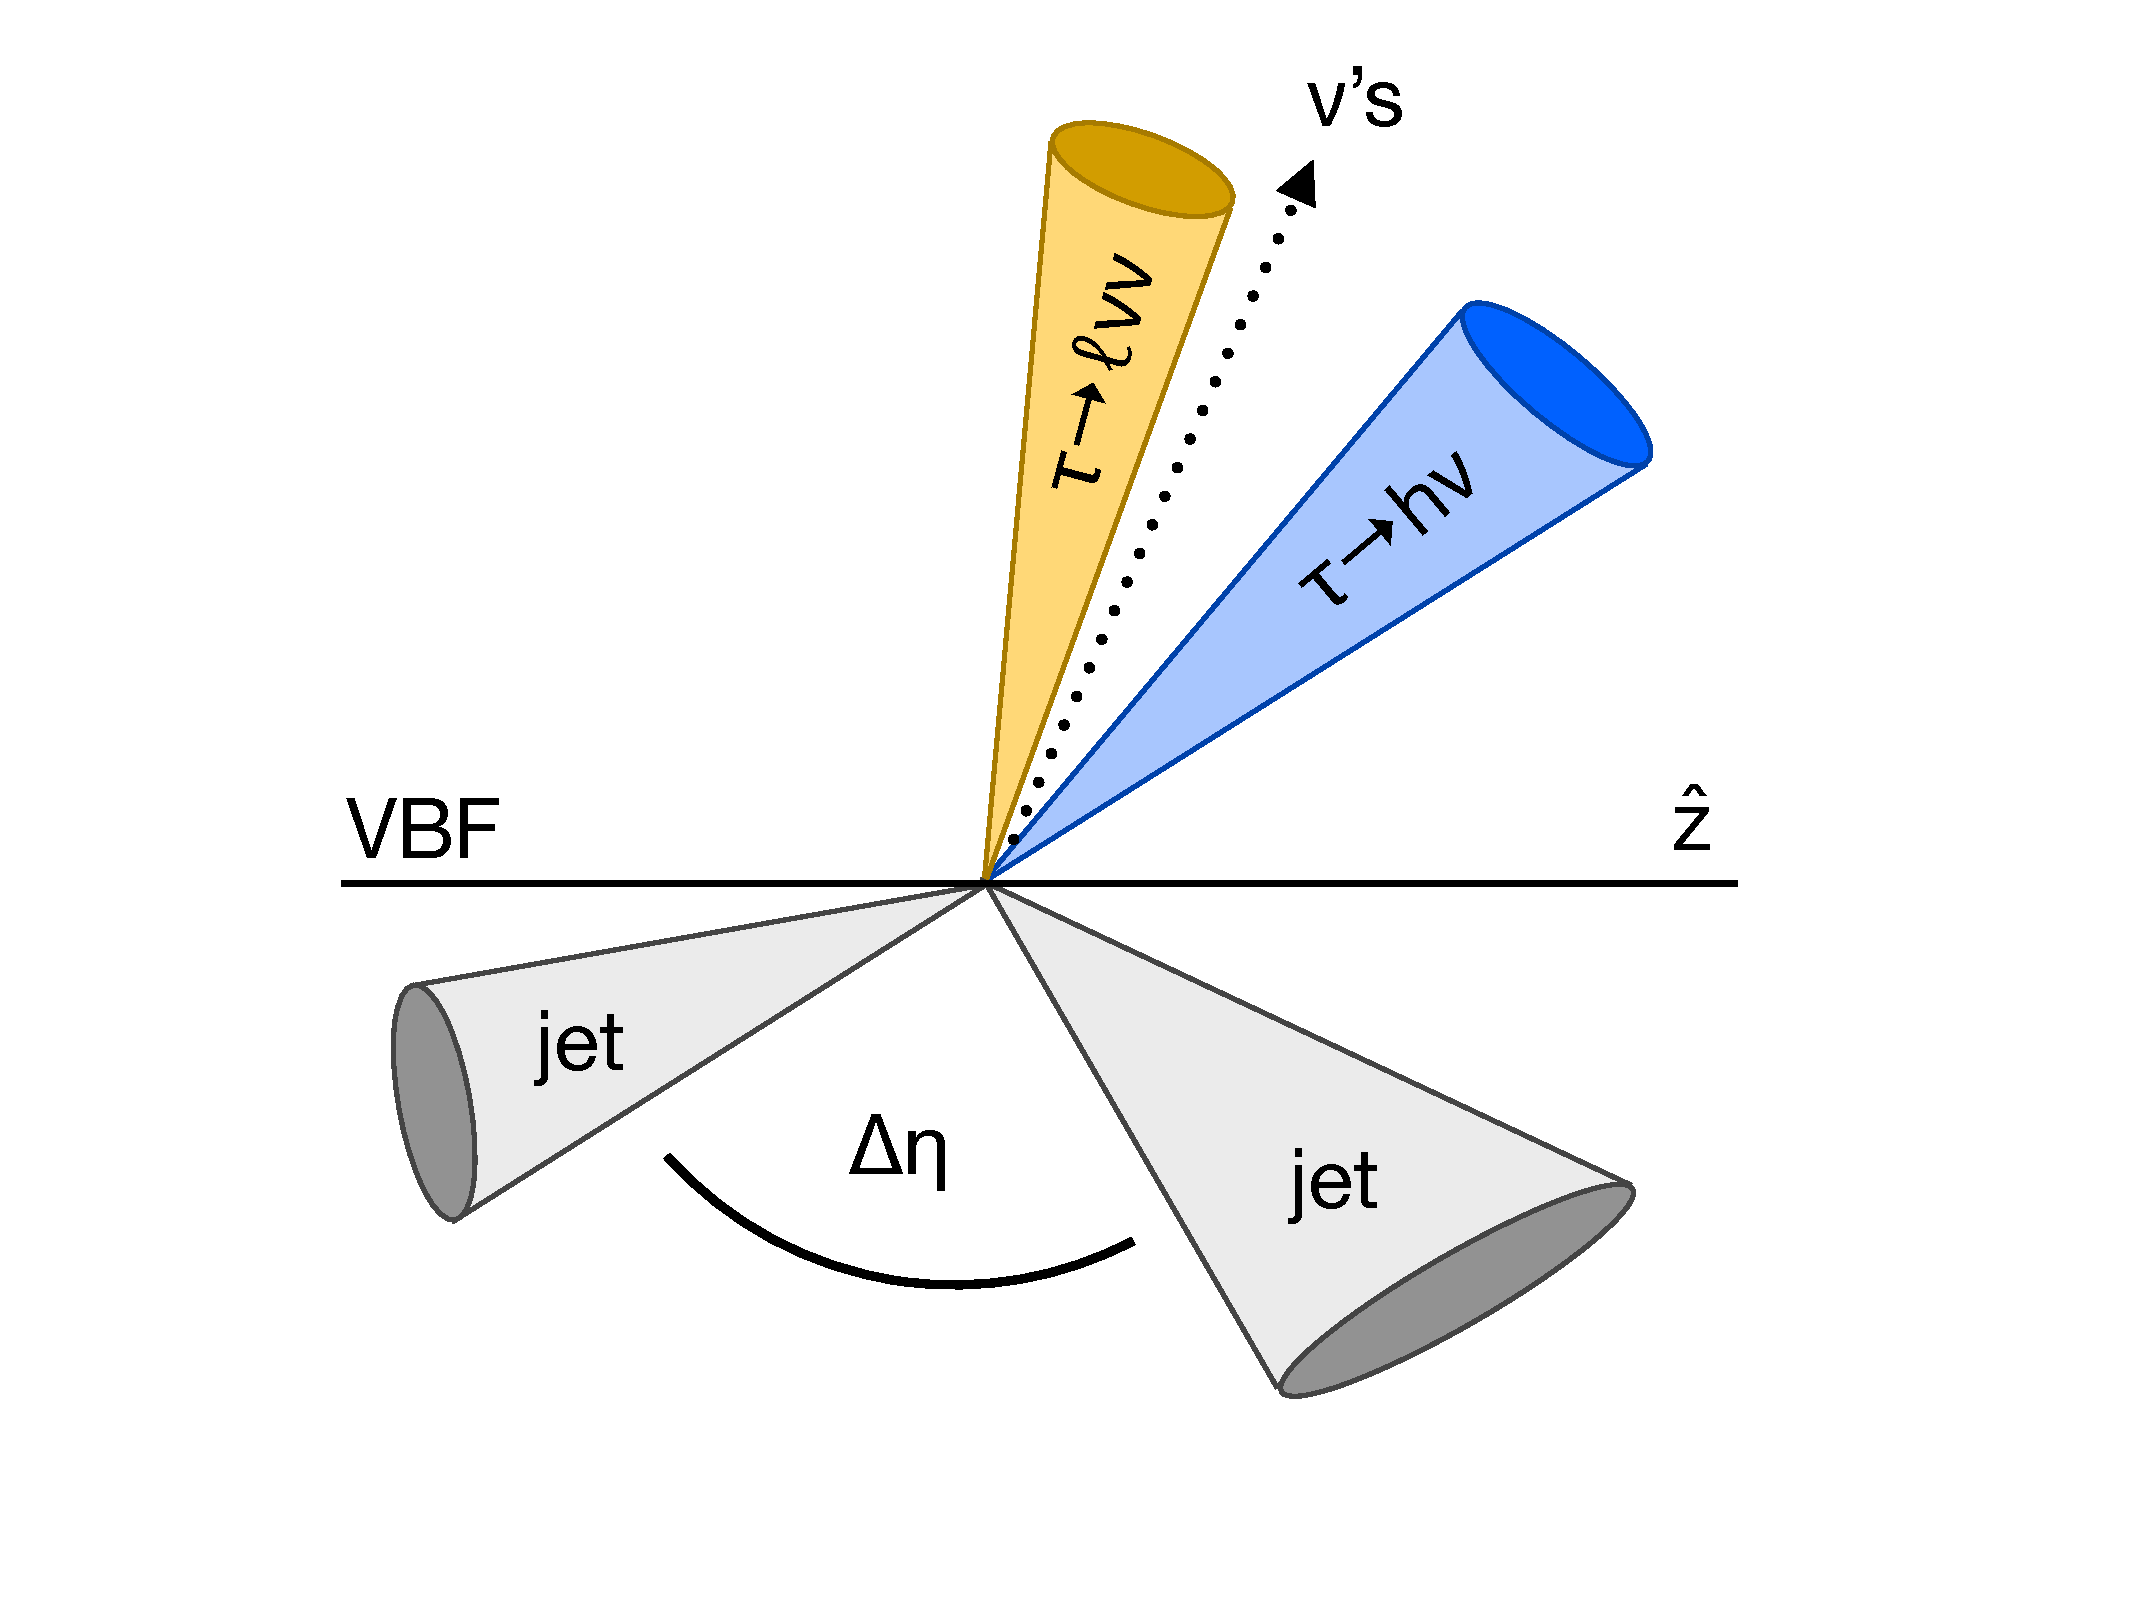
\includegraphics[width=0.48\textwidth]{figures/category-cartoons/vbf}
  \caption{Variables.}
  \label{fig:strategy-category-cartoons}
\end{figure}

\section{$\tautau$ mass reconstruction}
\label{sec:strategy-mtautau}

% mass ROCs
% ---------------------------------------------------------------------------------
\begin{figure}[tp]
  \centering
  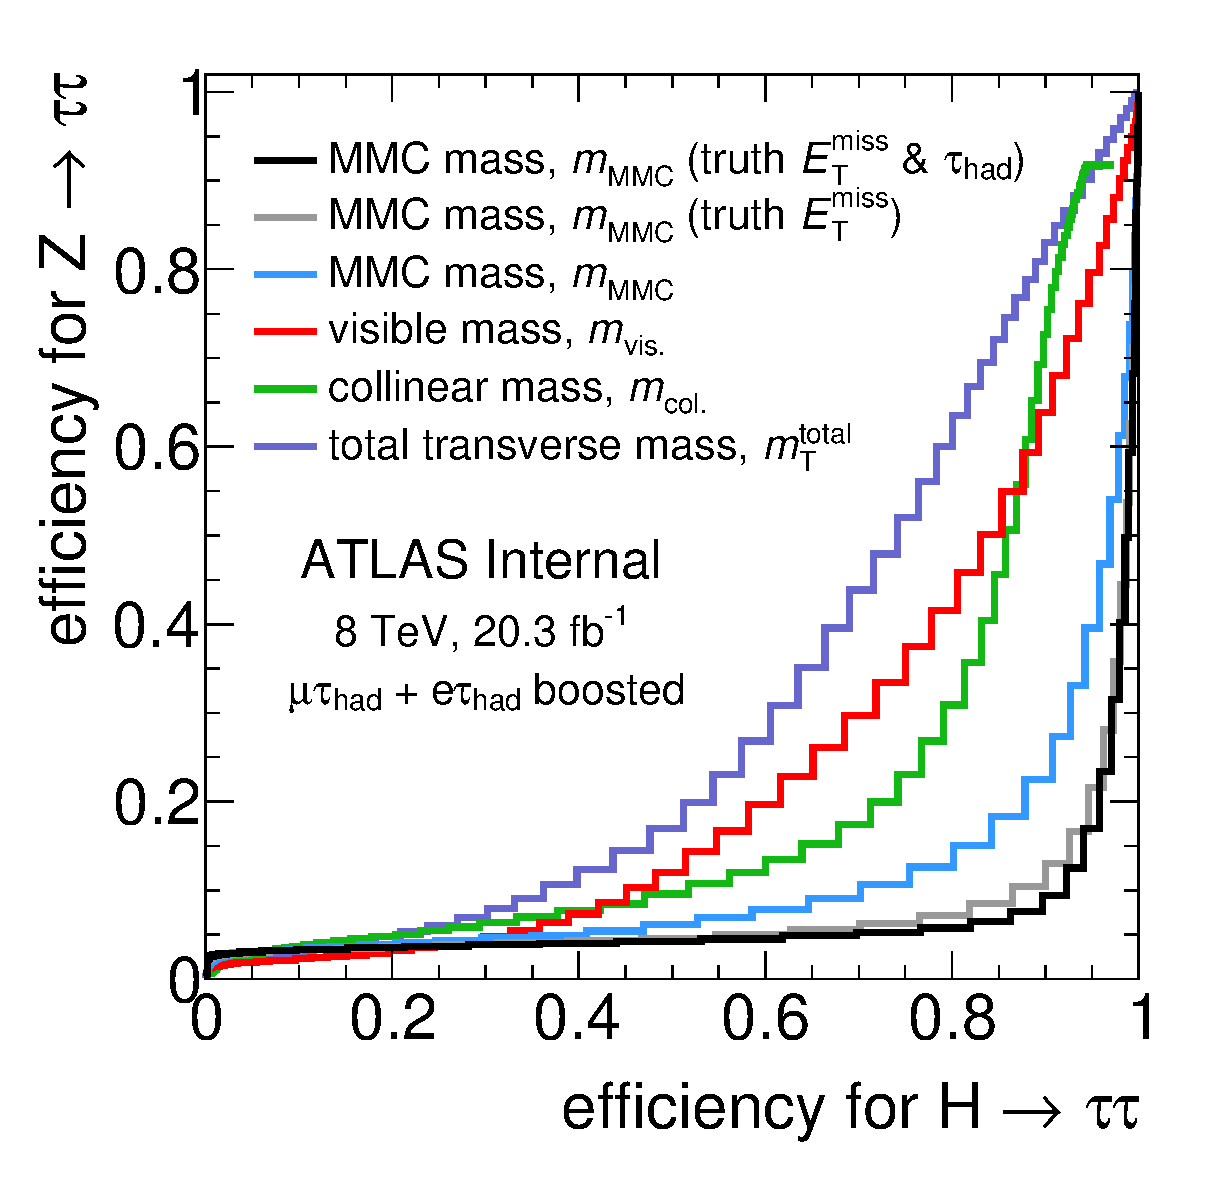
\includegraphics[width=0.48\textwidth]{figures/mtautau/mtautau-ROC-boost}
  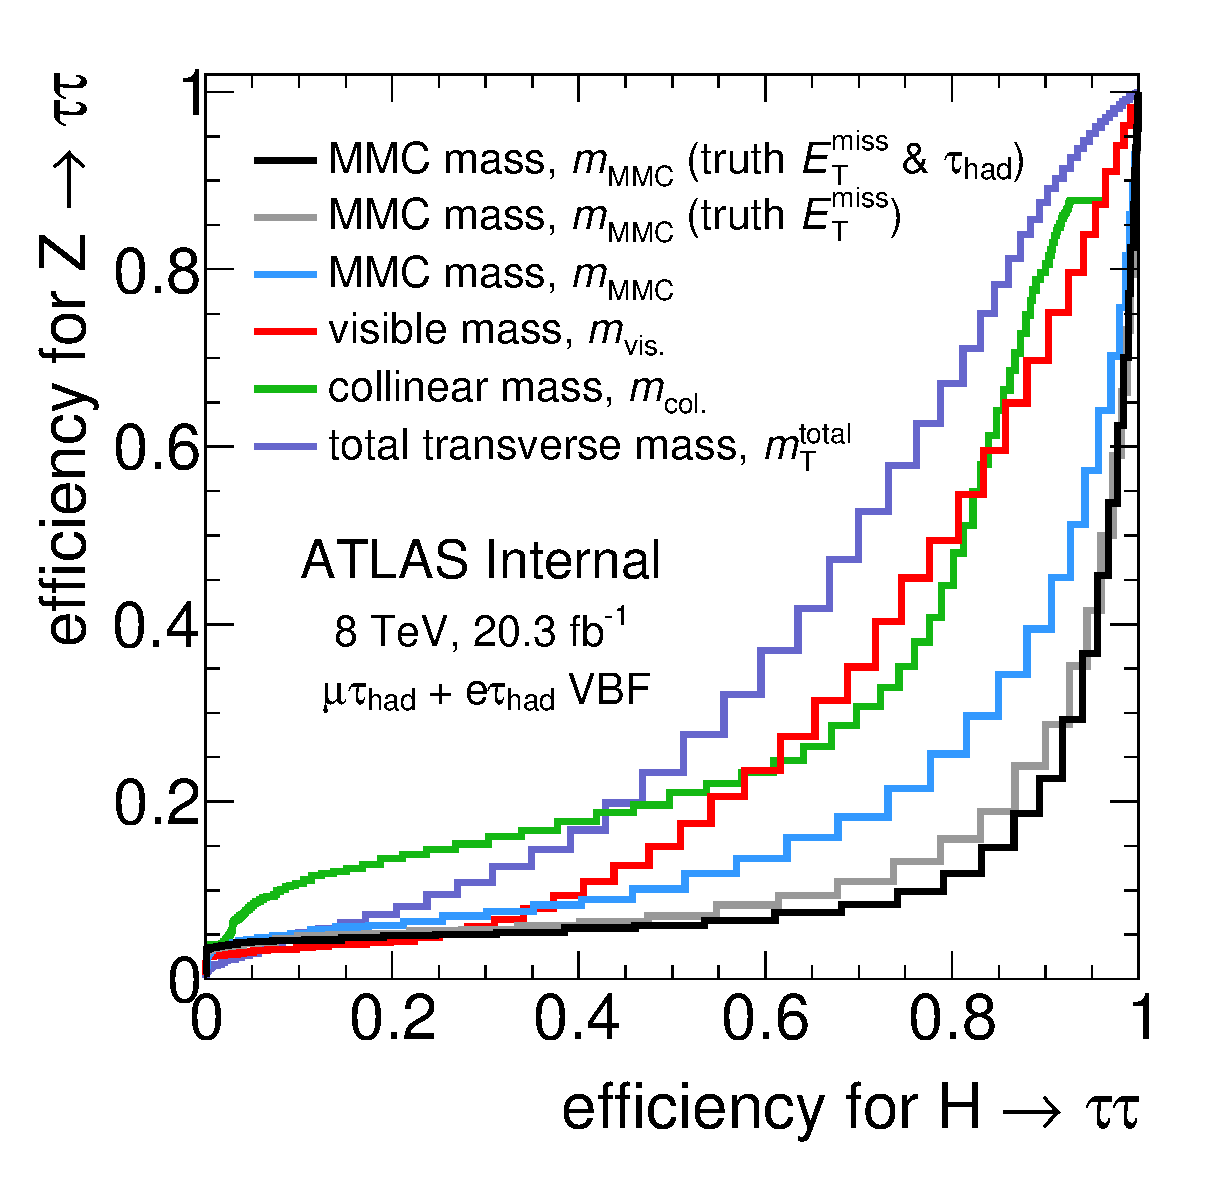
\includegraphics[width=0.48\textwidth]{figures/mtautau/mtautau-ROC-vbf}
  \caption{Variables.}
  \label{fig:strategy-mtautau-ROC}
\end{figure}
% ---------------------------------------------------------------------------------

\section{MVA discrimination}
\label{sec:strategy-mva}

% boost
% ---------------------------------------------------------------------------------
\begin{figure}[tp]
  \centering
  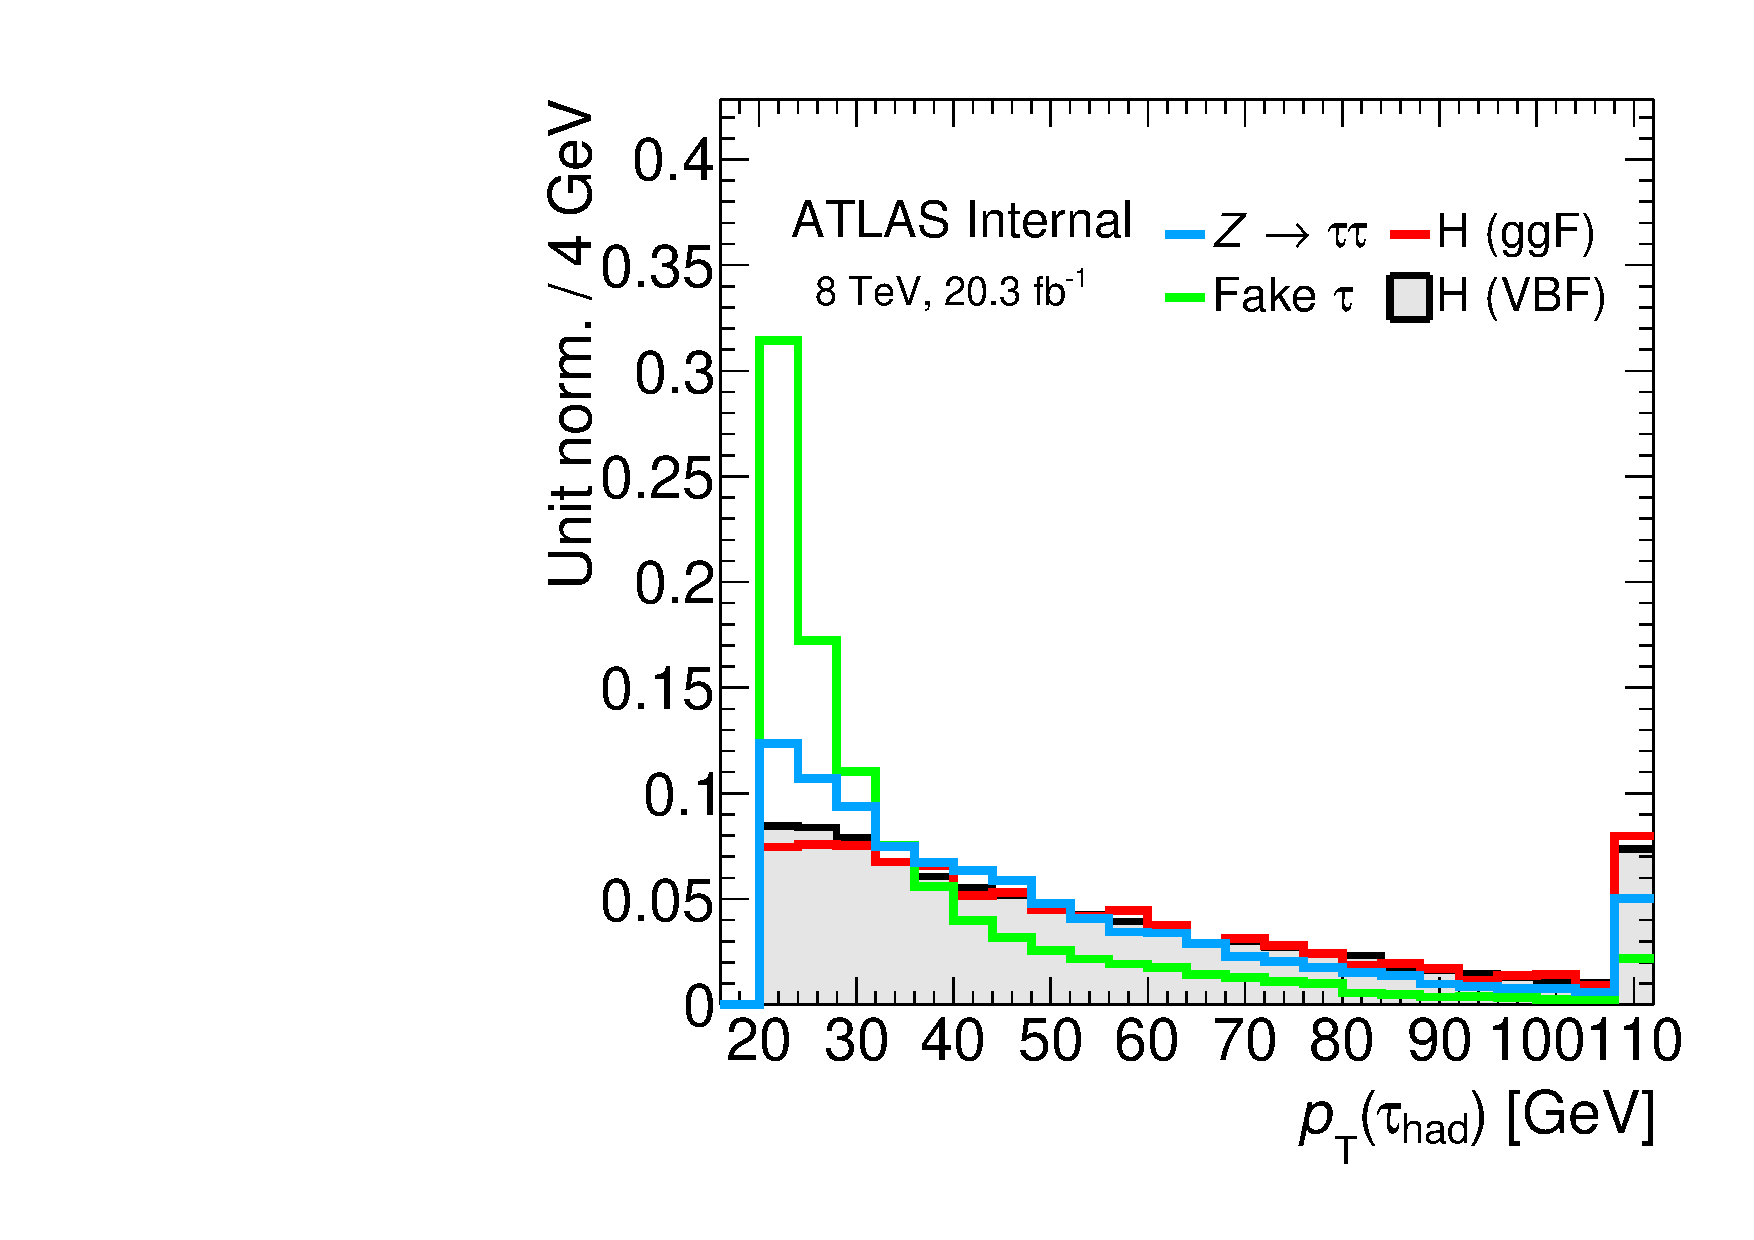
\includegraphics[width=0.35\textwidth]{figures/overlaid/boost/tau-pt}
  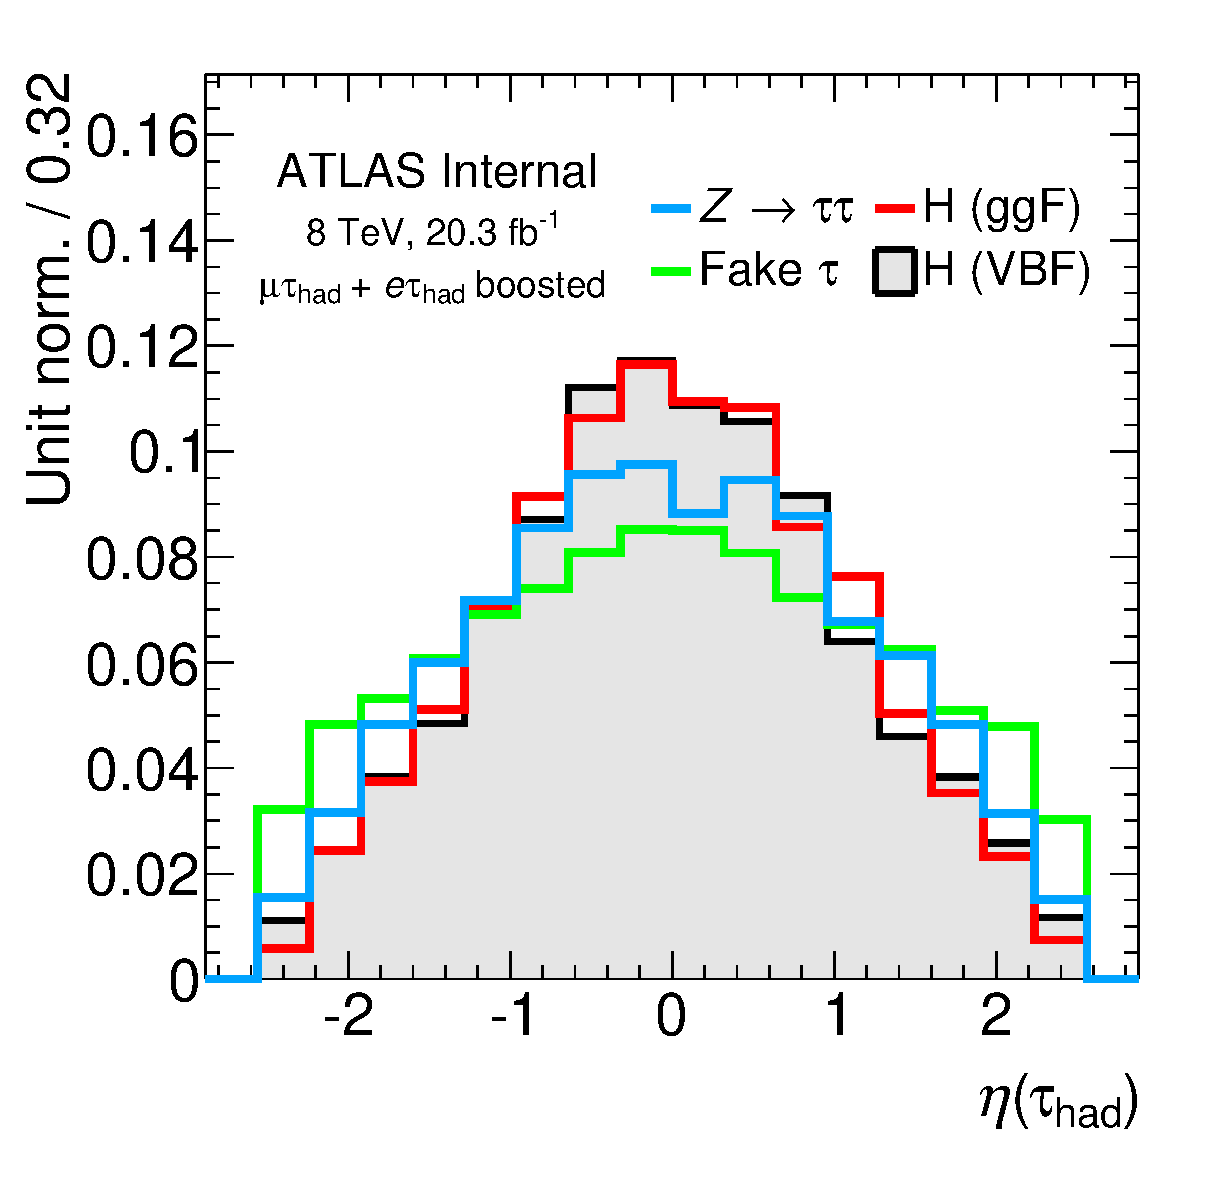
\includegraphics[width=0.35\textwidth]{figures/overlaid/boost/tau-eta}
  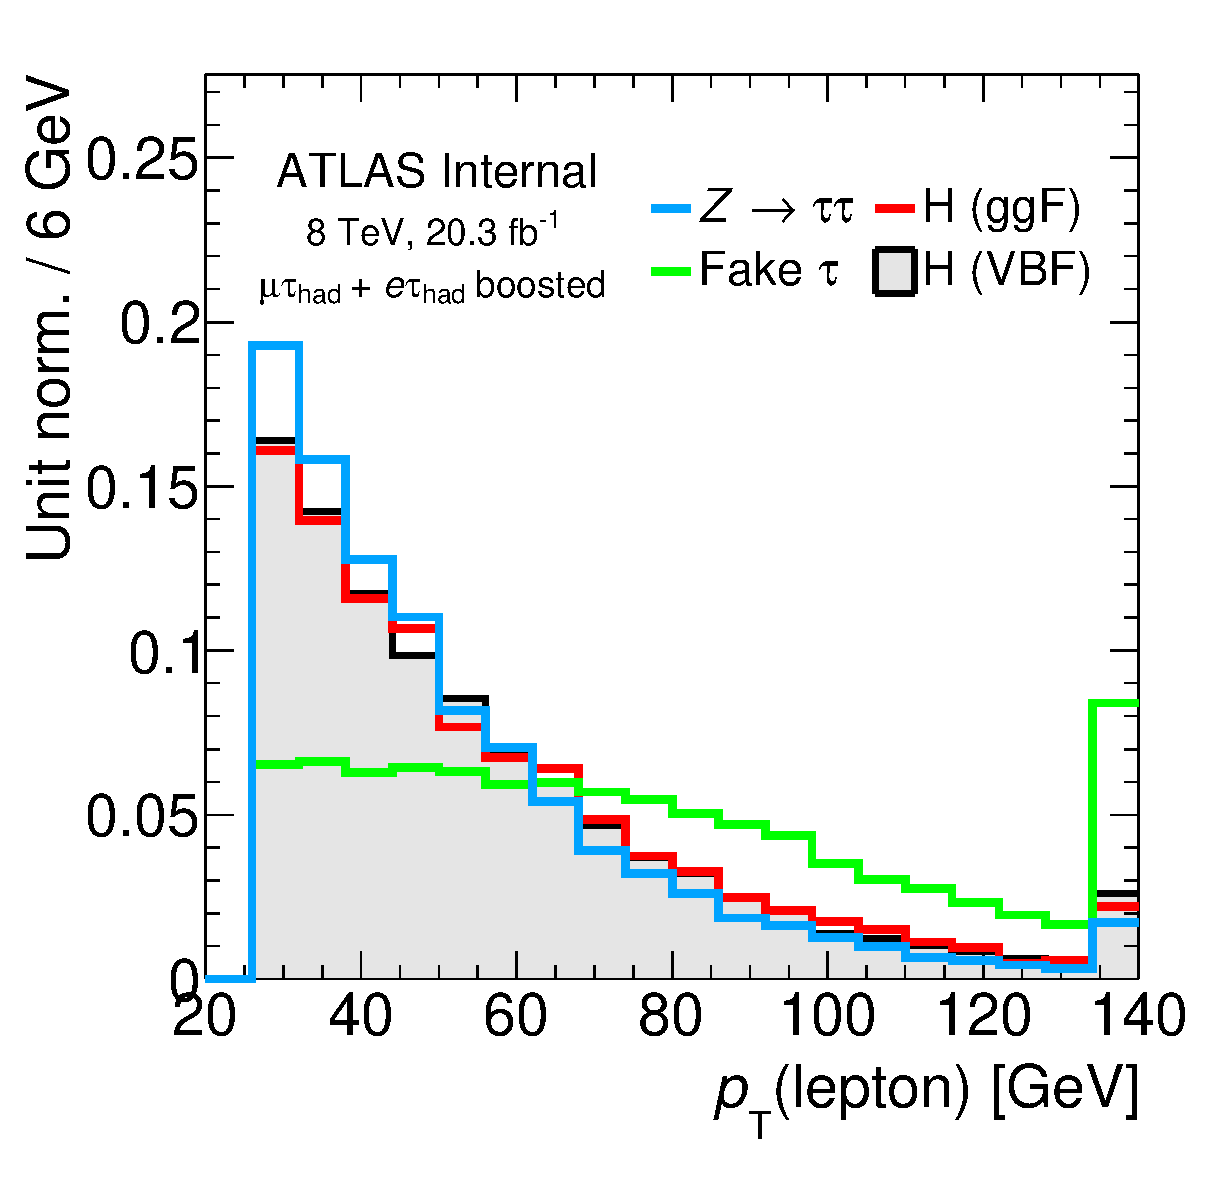
\includegraphics[width=0.35\textwidth]{figures/overlaid/boost/lep-pt-hi}
  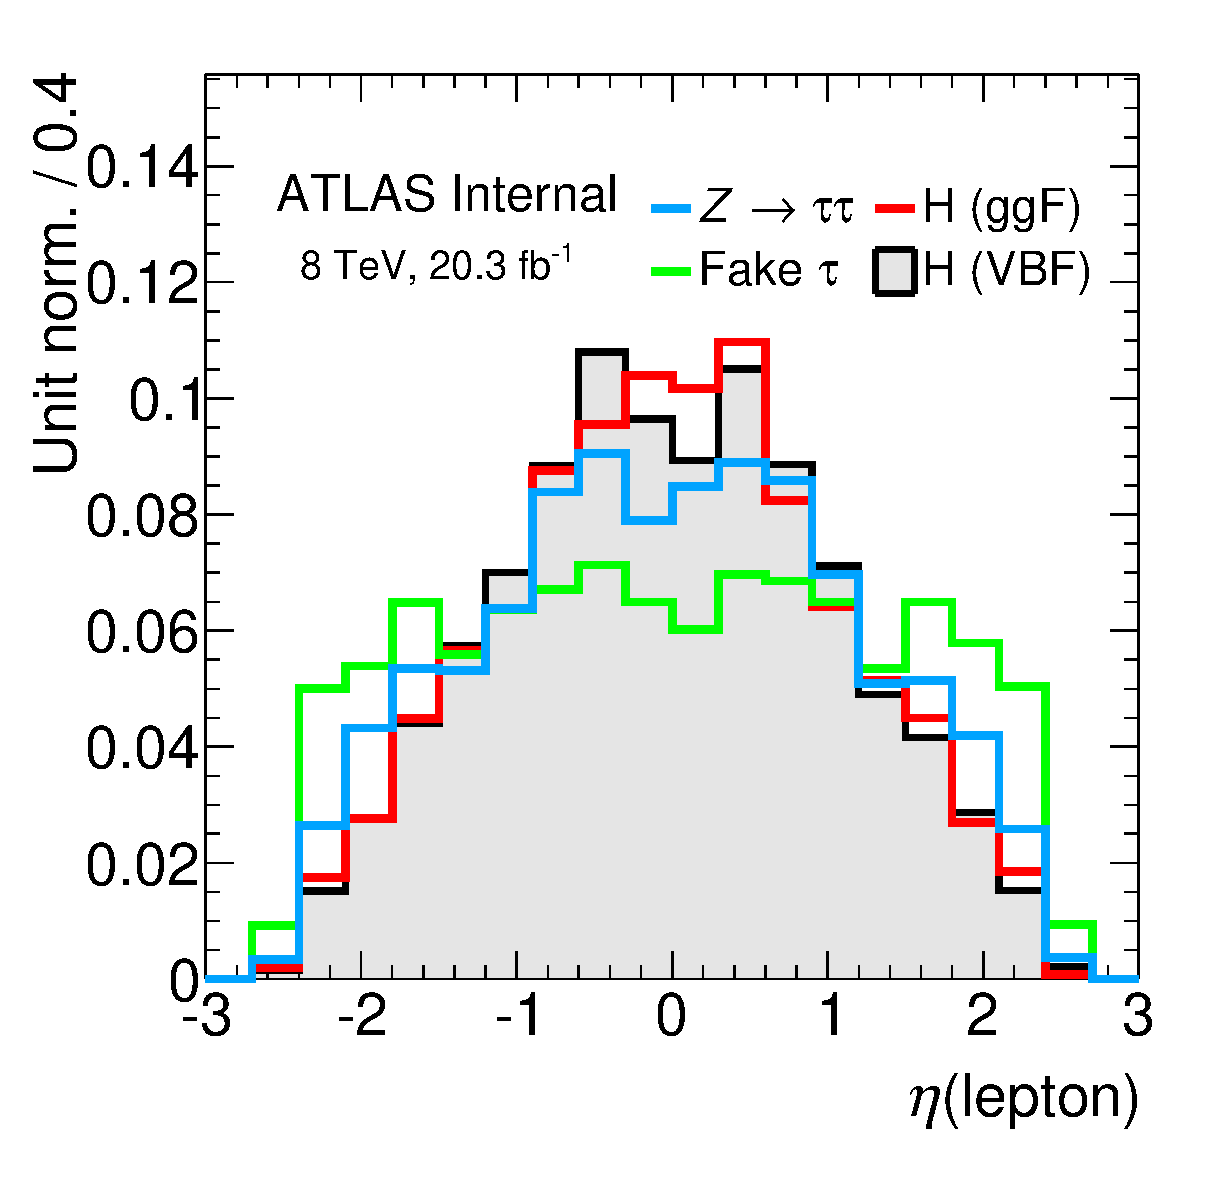
\includegraphics[width=0.35\textwidth]{figures/overlaid/boost/lep-eta}
  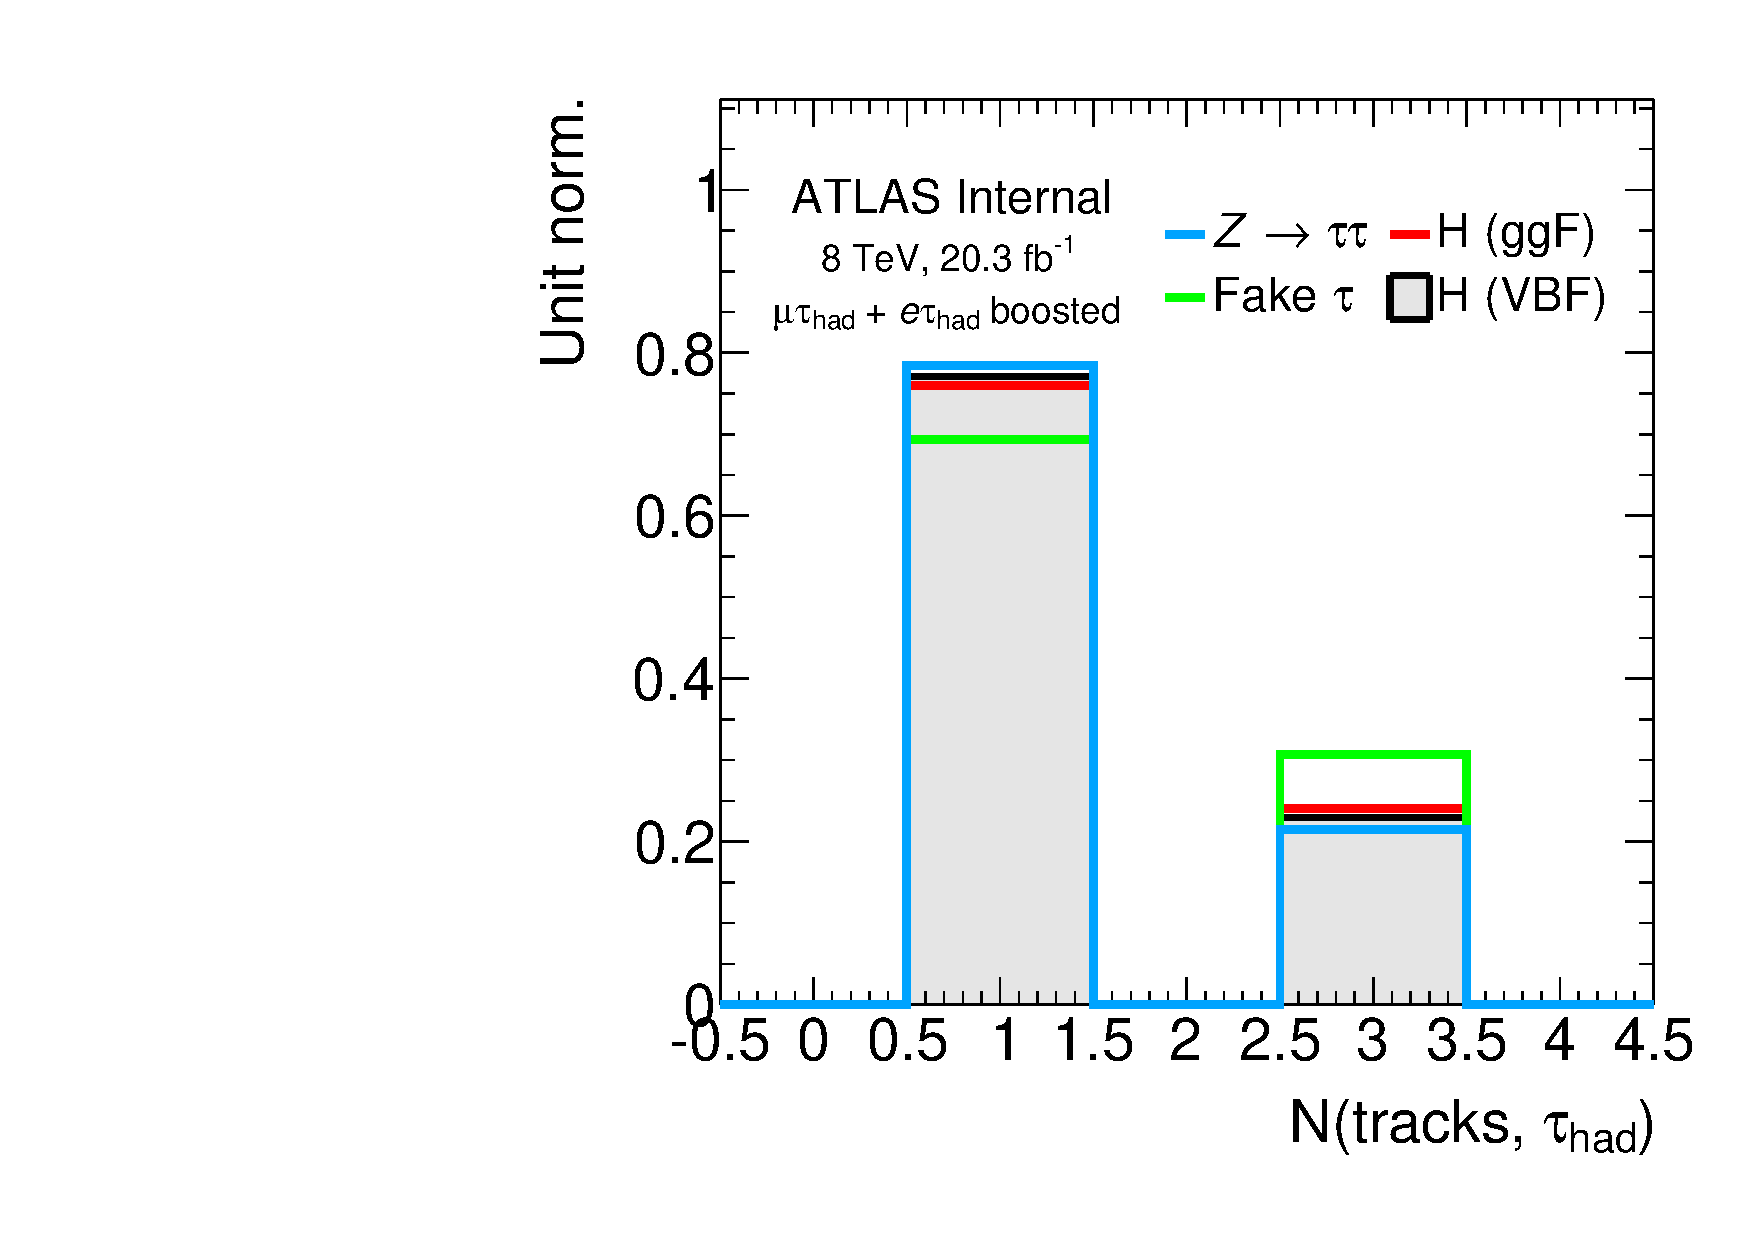
\includegraphics[width=0.35\textwidth]{figures/overlaid/boost/tau-numTrack}
  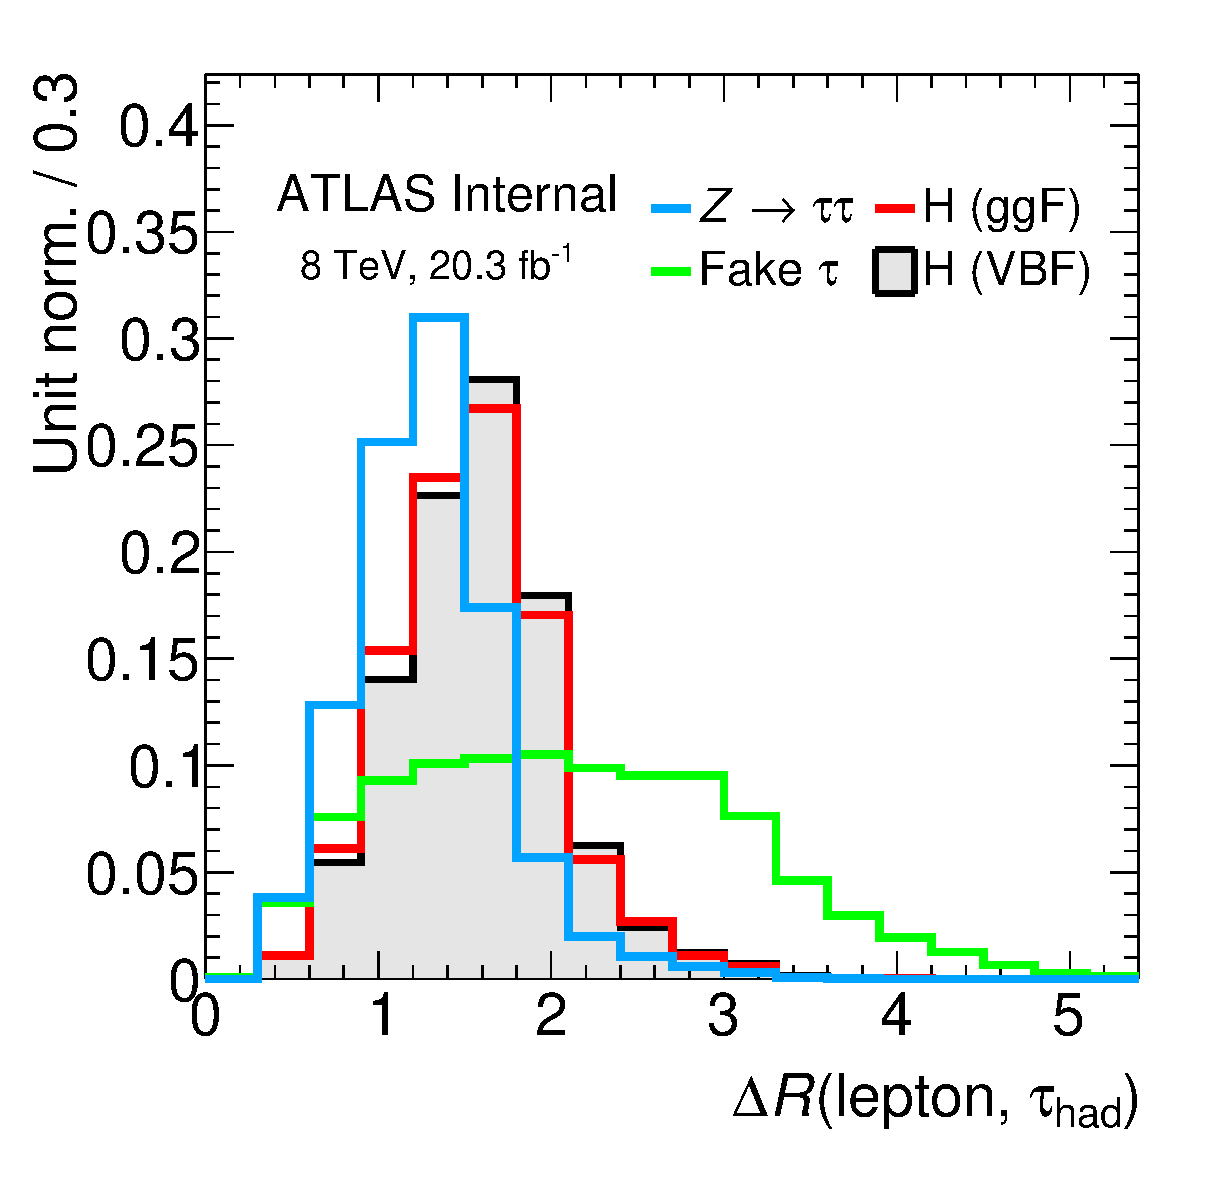
\includegraphics[width=0.35\textwidth]{figures/overlaid/boost/taulep-dR}
  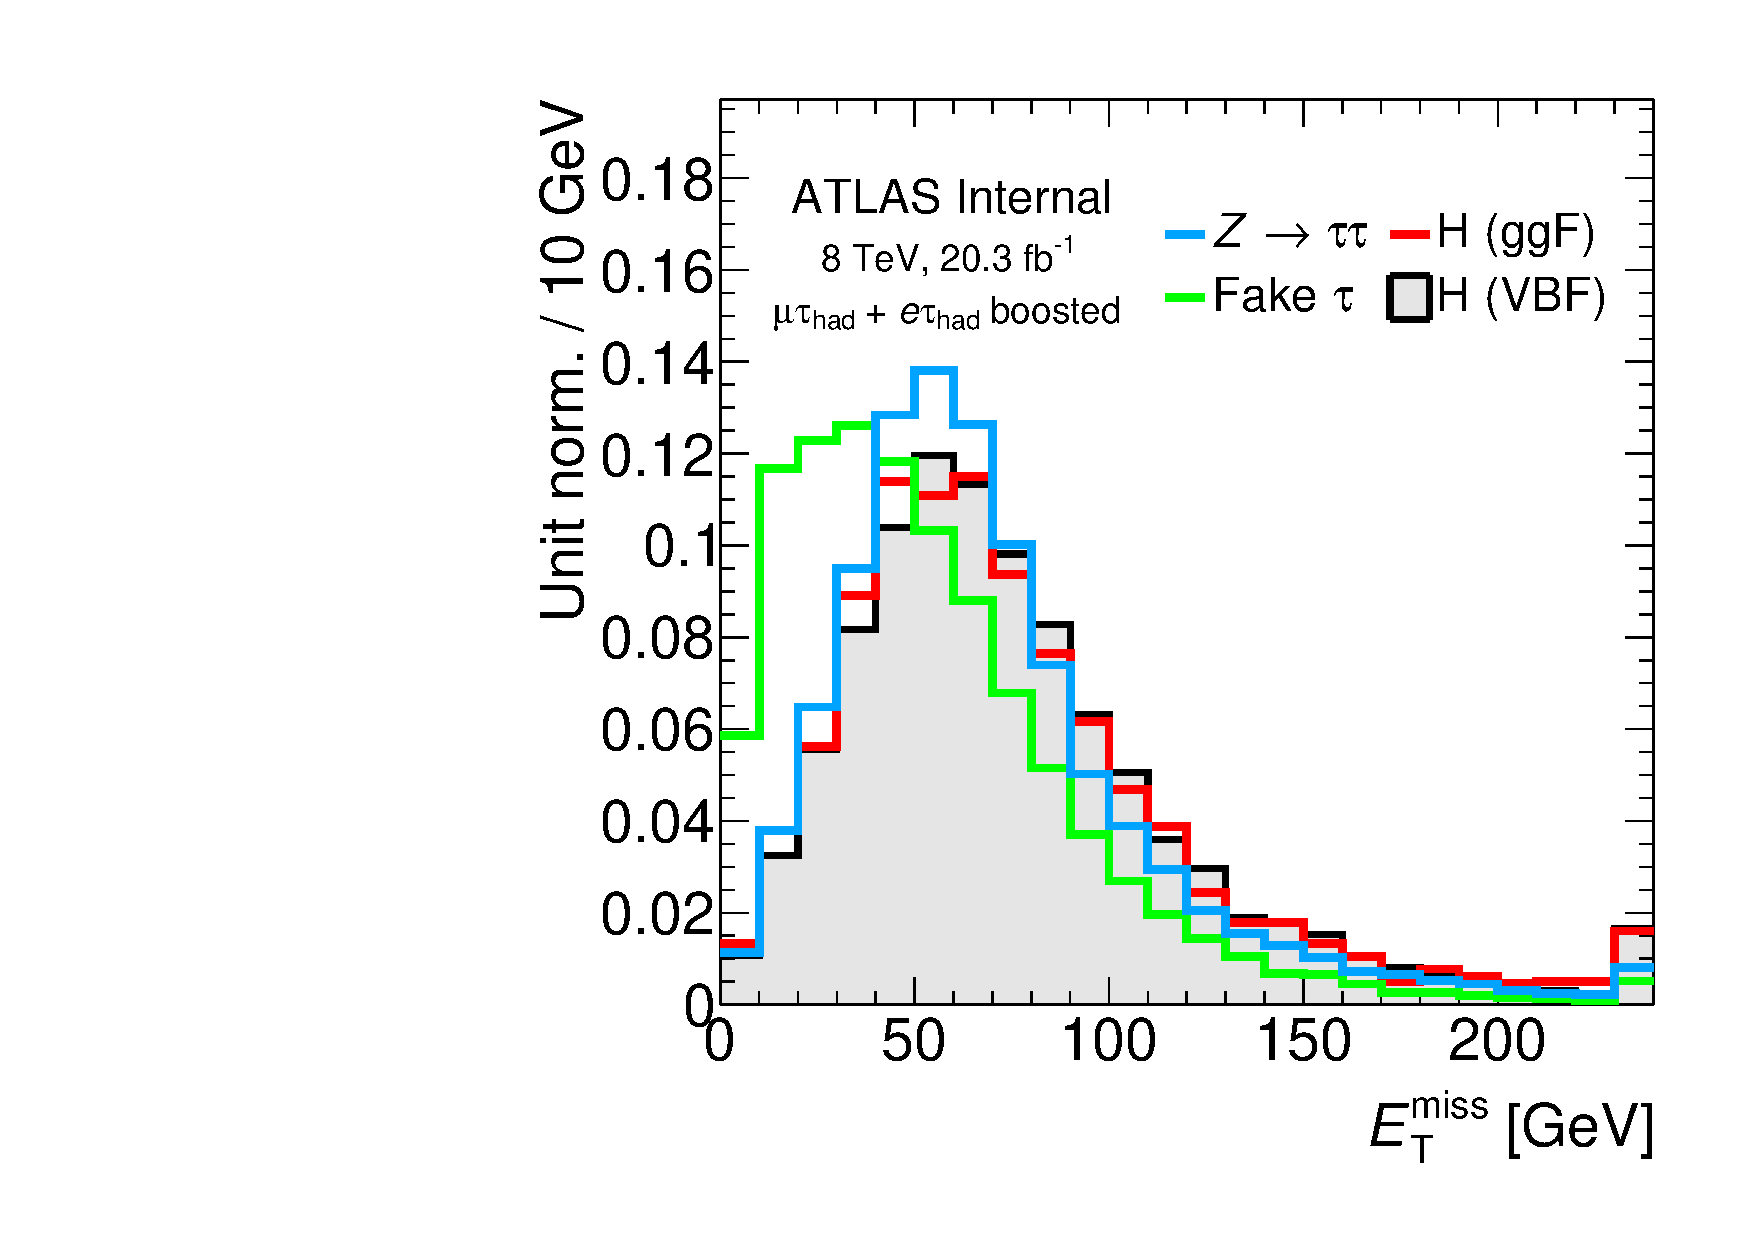
\includegraphics[width=0.35\textwidth]{figures/overlaid/boost/met-pt-hi}
  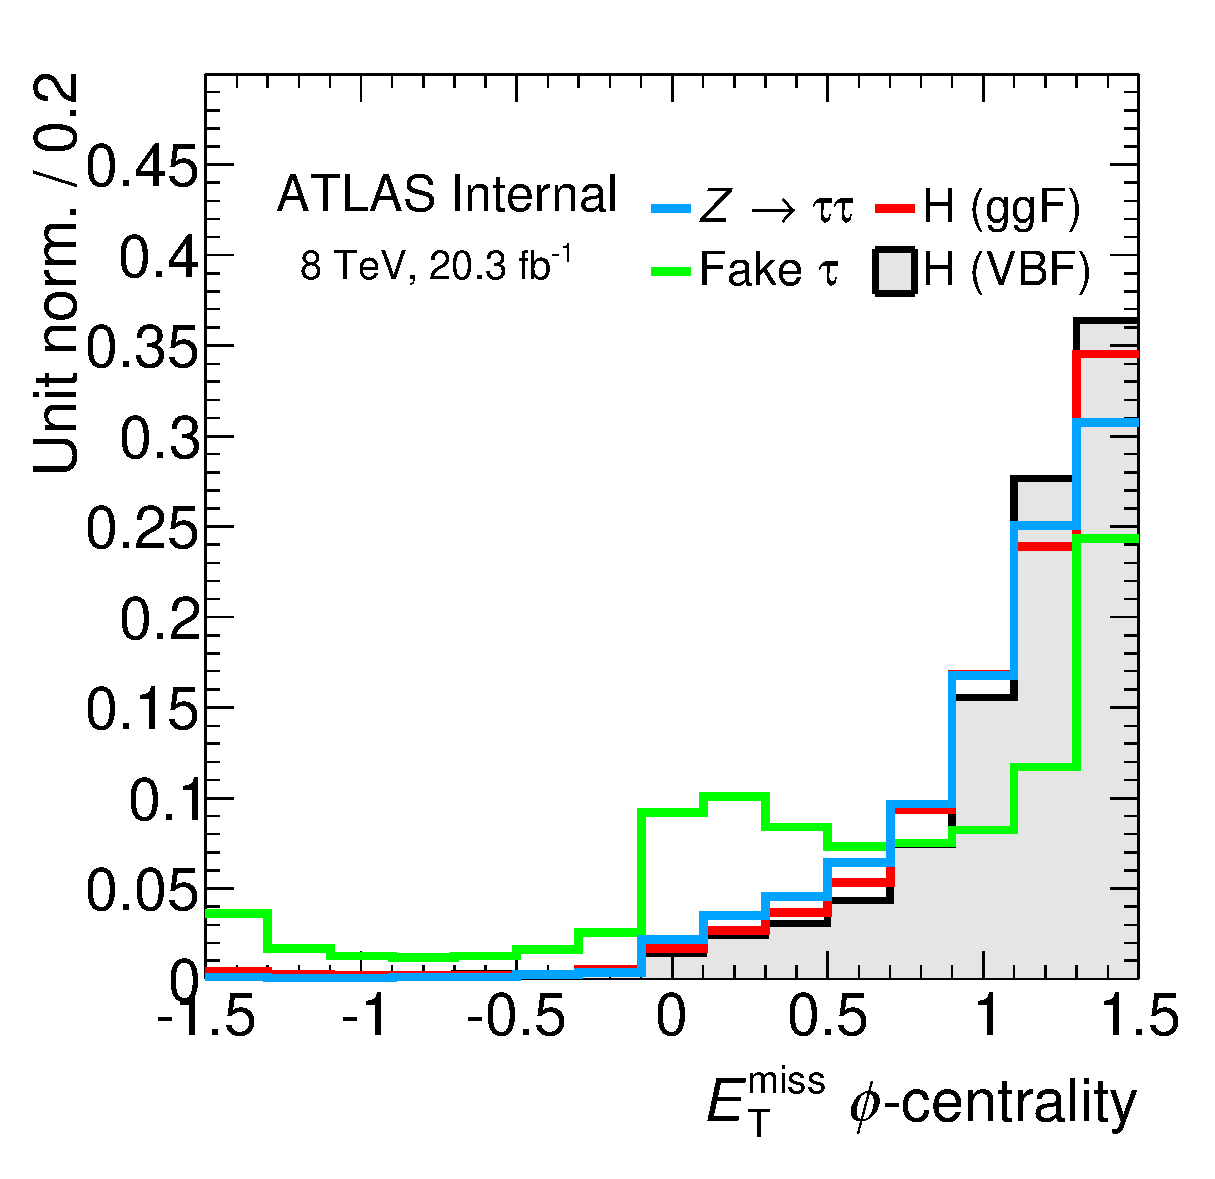
\includegraphics[width=0.35\textwidth]{figures/overlaid/boost/met-phi-centrality}
  \caption{Variables.}
  \label{fig:strategy-overlaid-boost-taus}
\end{figure}
\begin{figure}[tp]
  \centering
  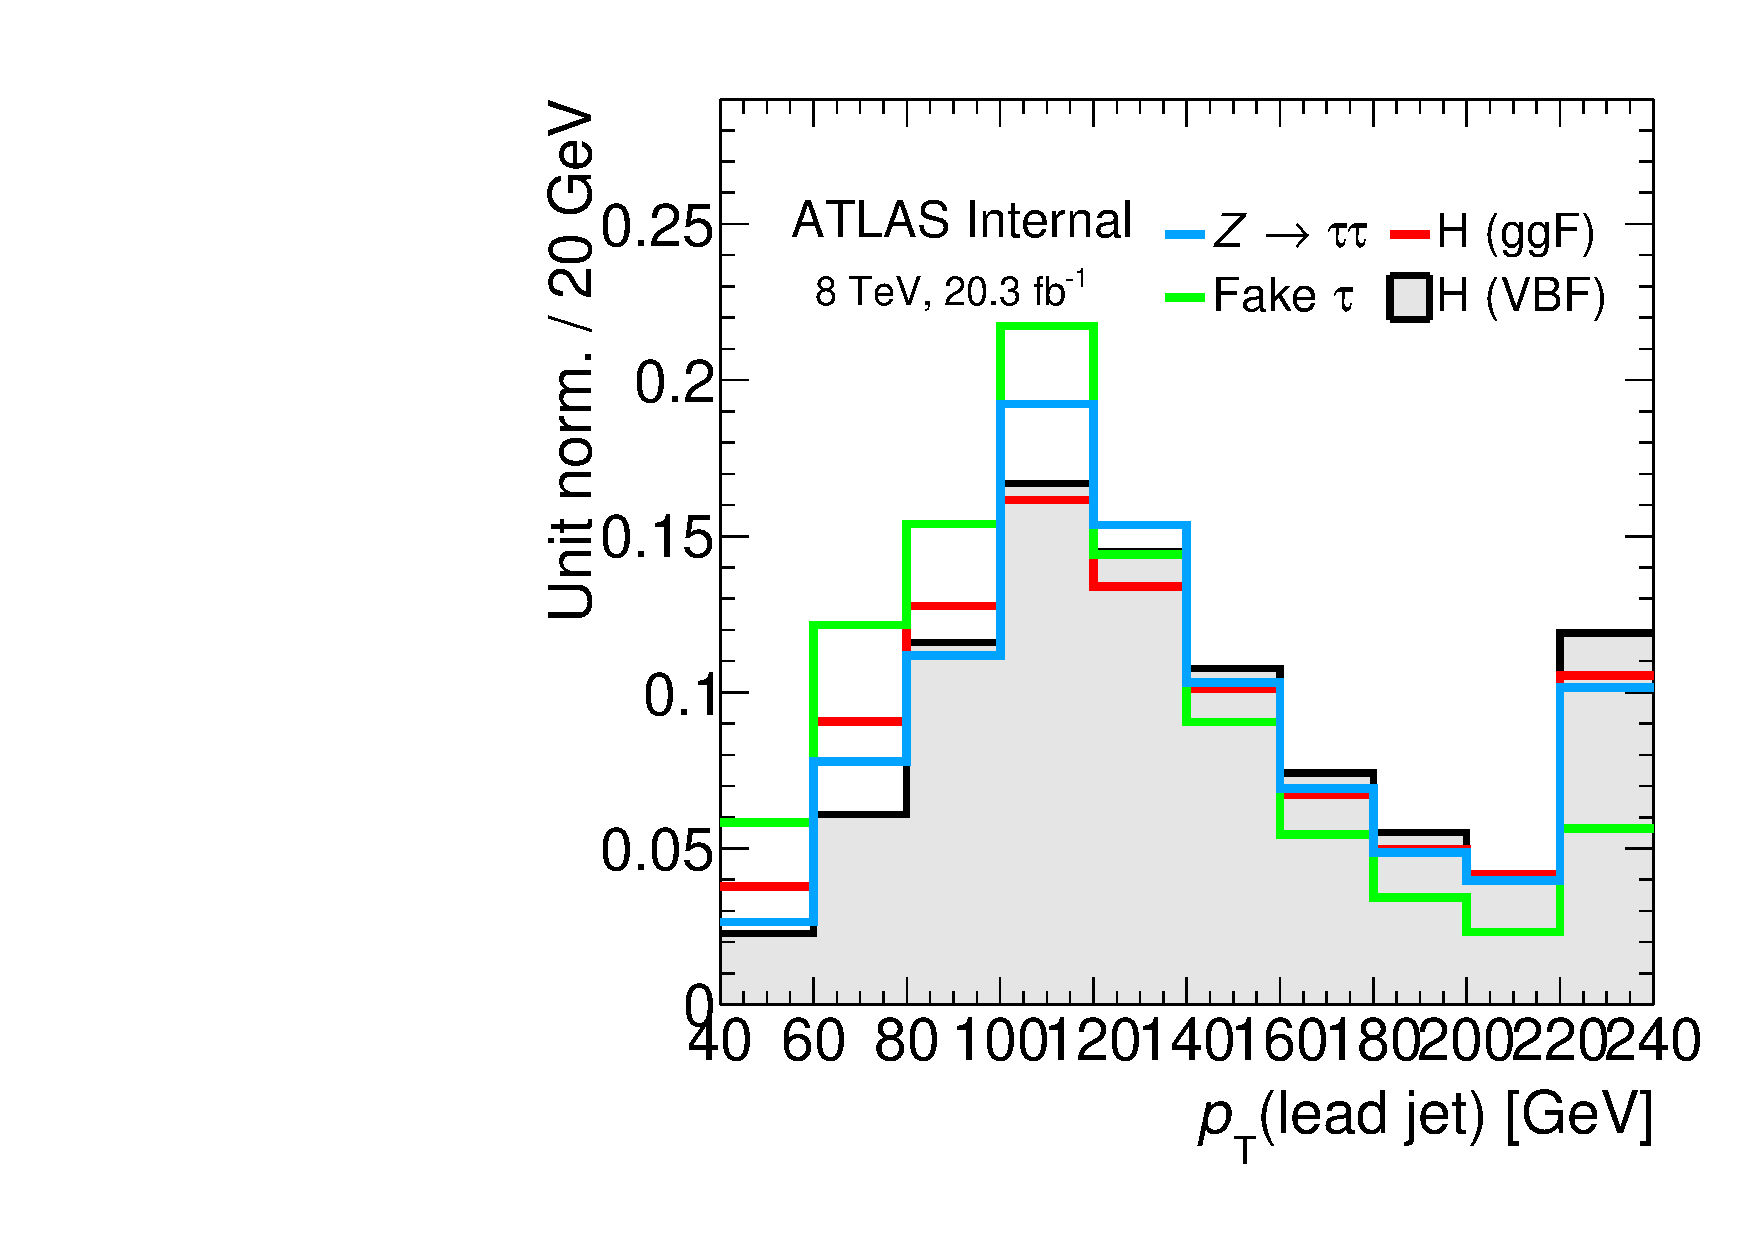
\includegraphics[width=0.45\textwidth]{figures/overlaid/boost/jet-1-pt}
  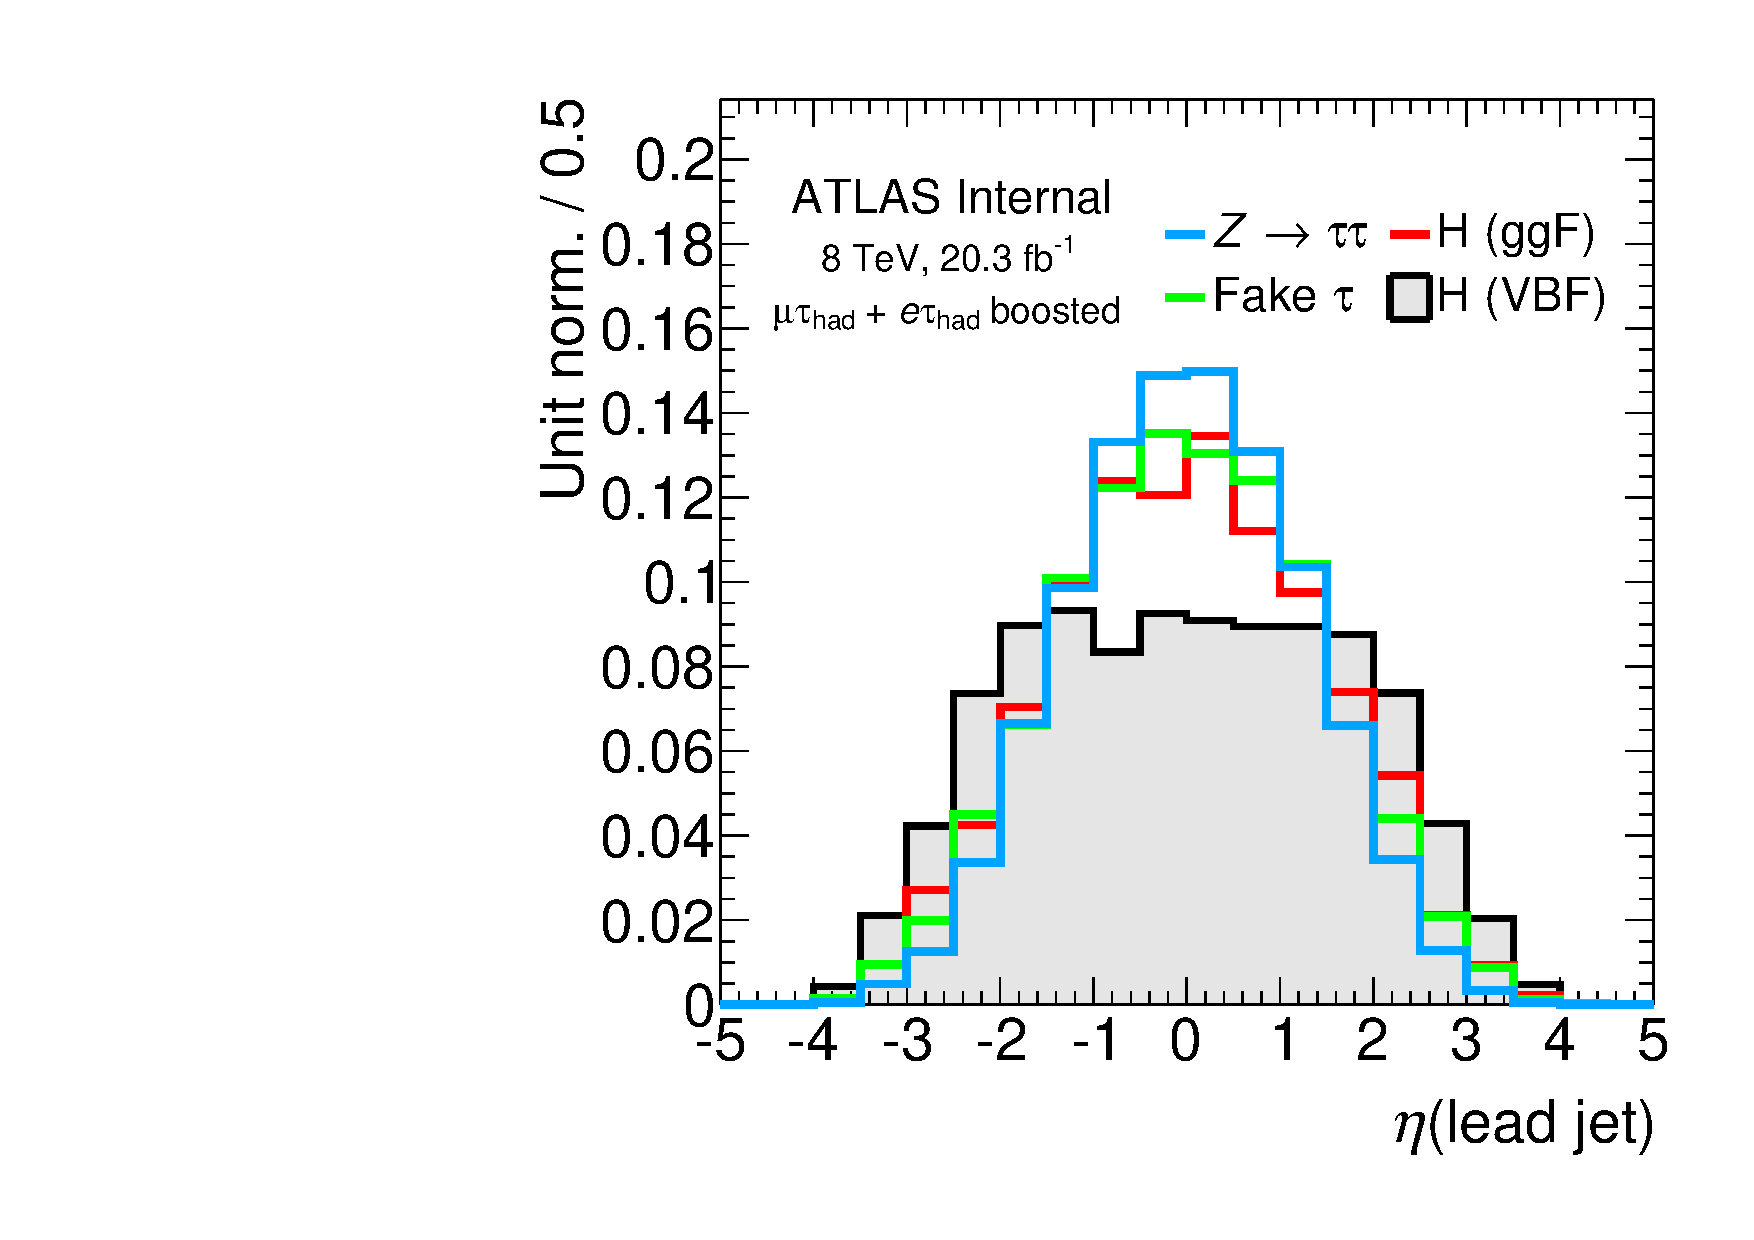
\includegraphics[width=0.45\textwidth]{figures/overlaid/boost/jet-1-eta}
  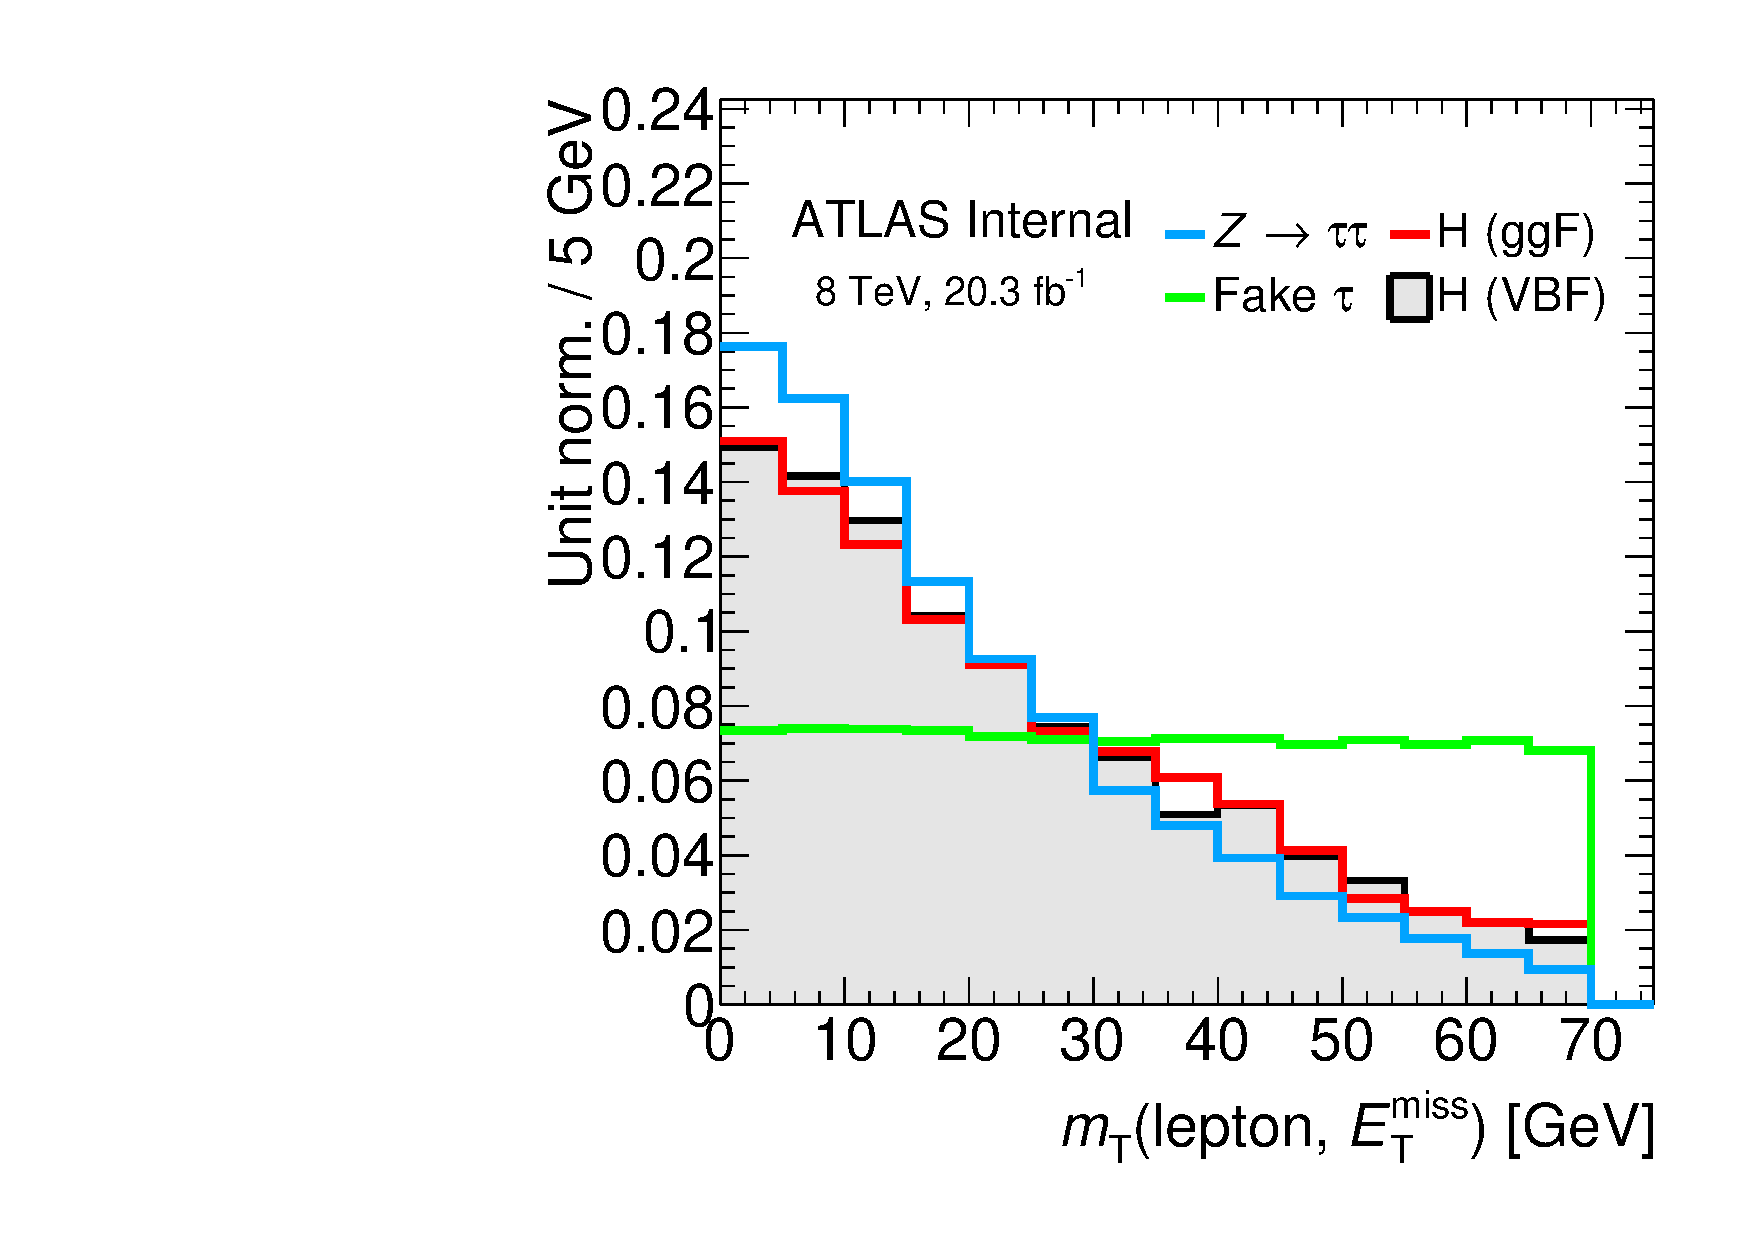
\includegraphics[width=0.45\textwidth]{figures/overlaid/boost/mT}
  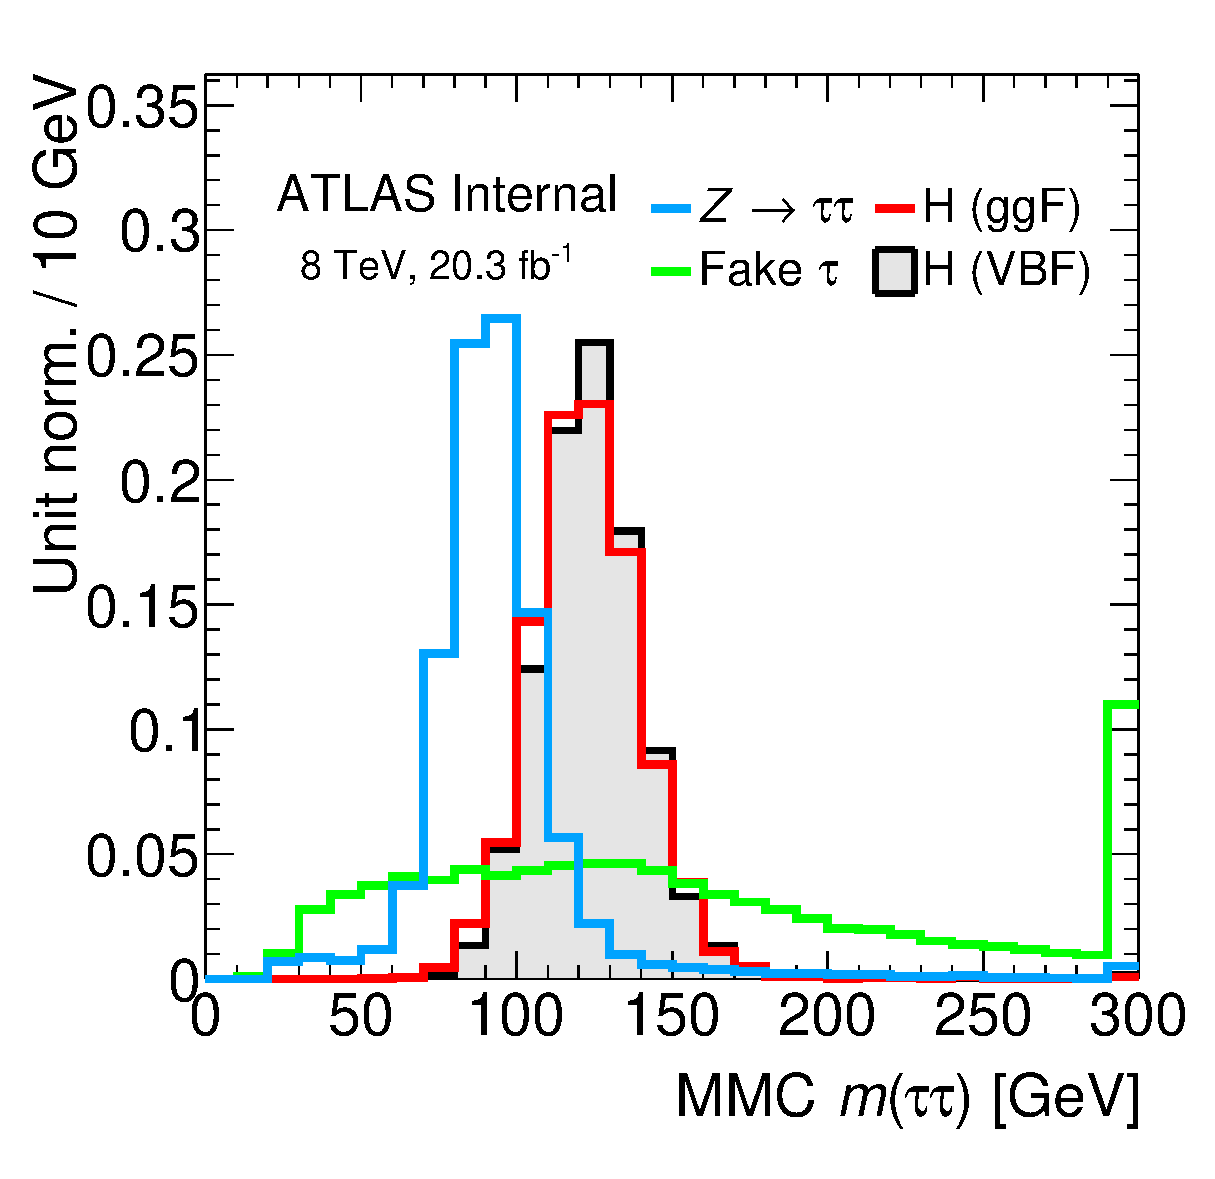
\includegraphics[width=0.45\textwidth]{figures/overlaid/boost/mMMC}
  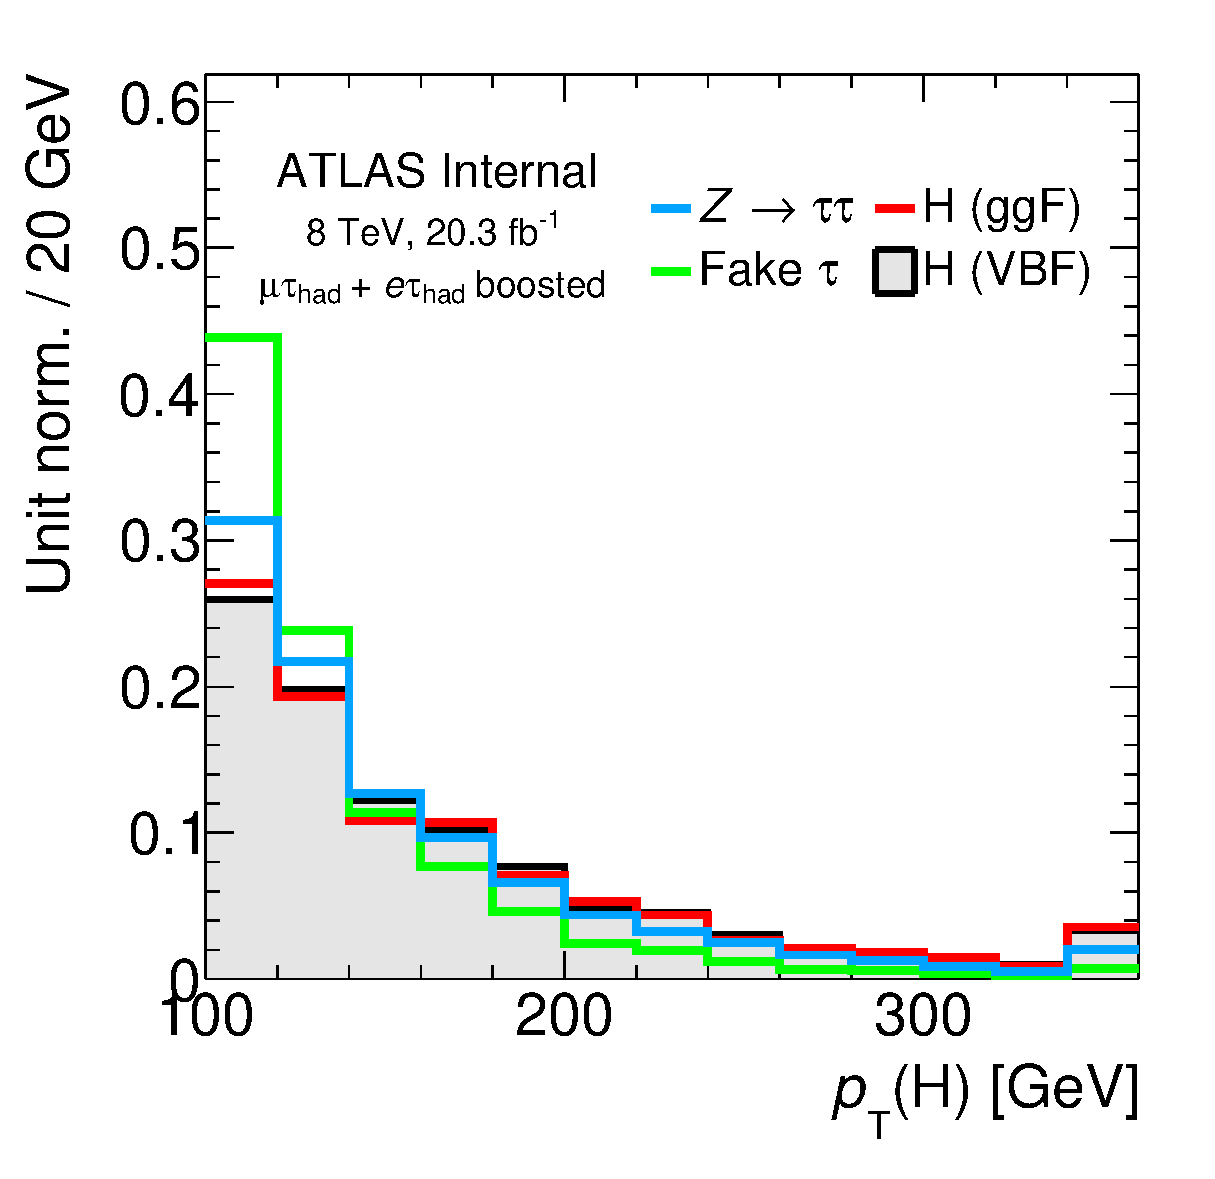
\includegraphics[width=0.45\textwidth]{figures/overlaid/boost/H-pt-hi}
  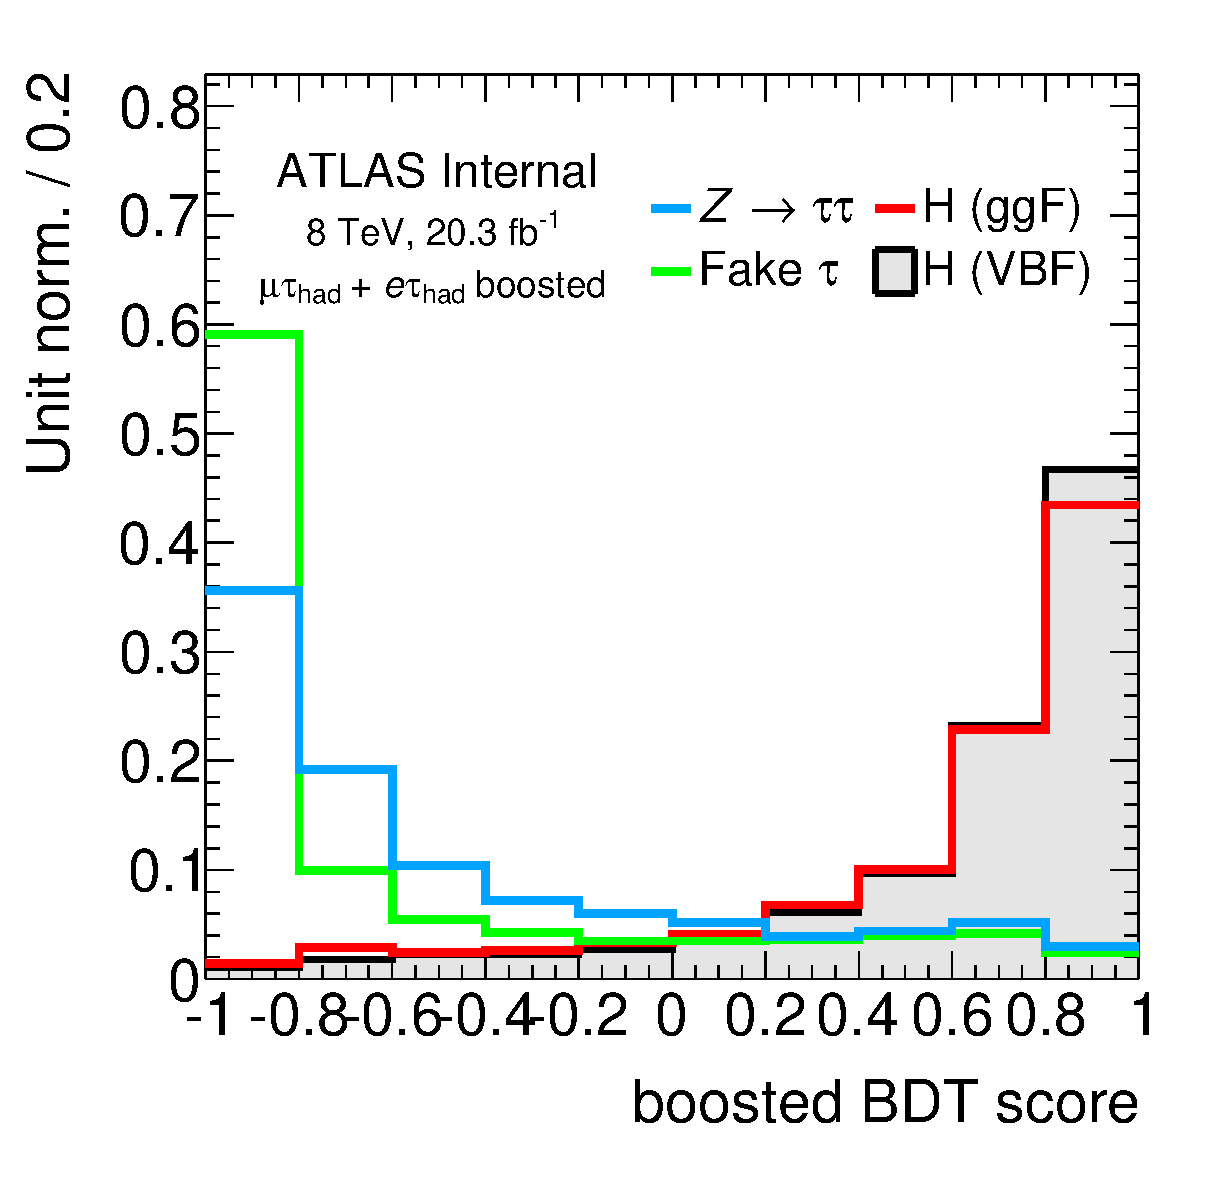
\includegraphics[width=0.45\textwidth]{figures/overlaid/boost/BDTEve-boost}
  \caption{Variables.}
  \label{fig:strategy-overlaid-boost-other}
\end{figure}
% ---------------------------------------------------------------------------------

% VBF
% ---------------------------------------------------------------------------------

\begin{figure}[tp]
  \centering
  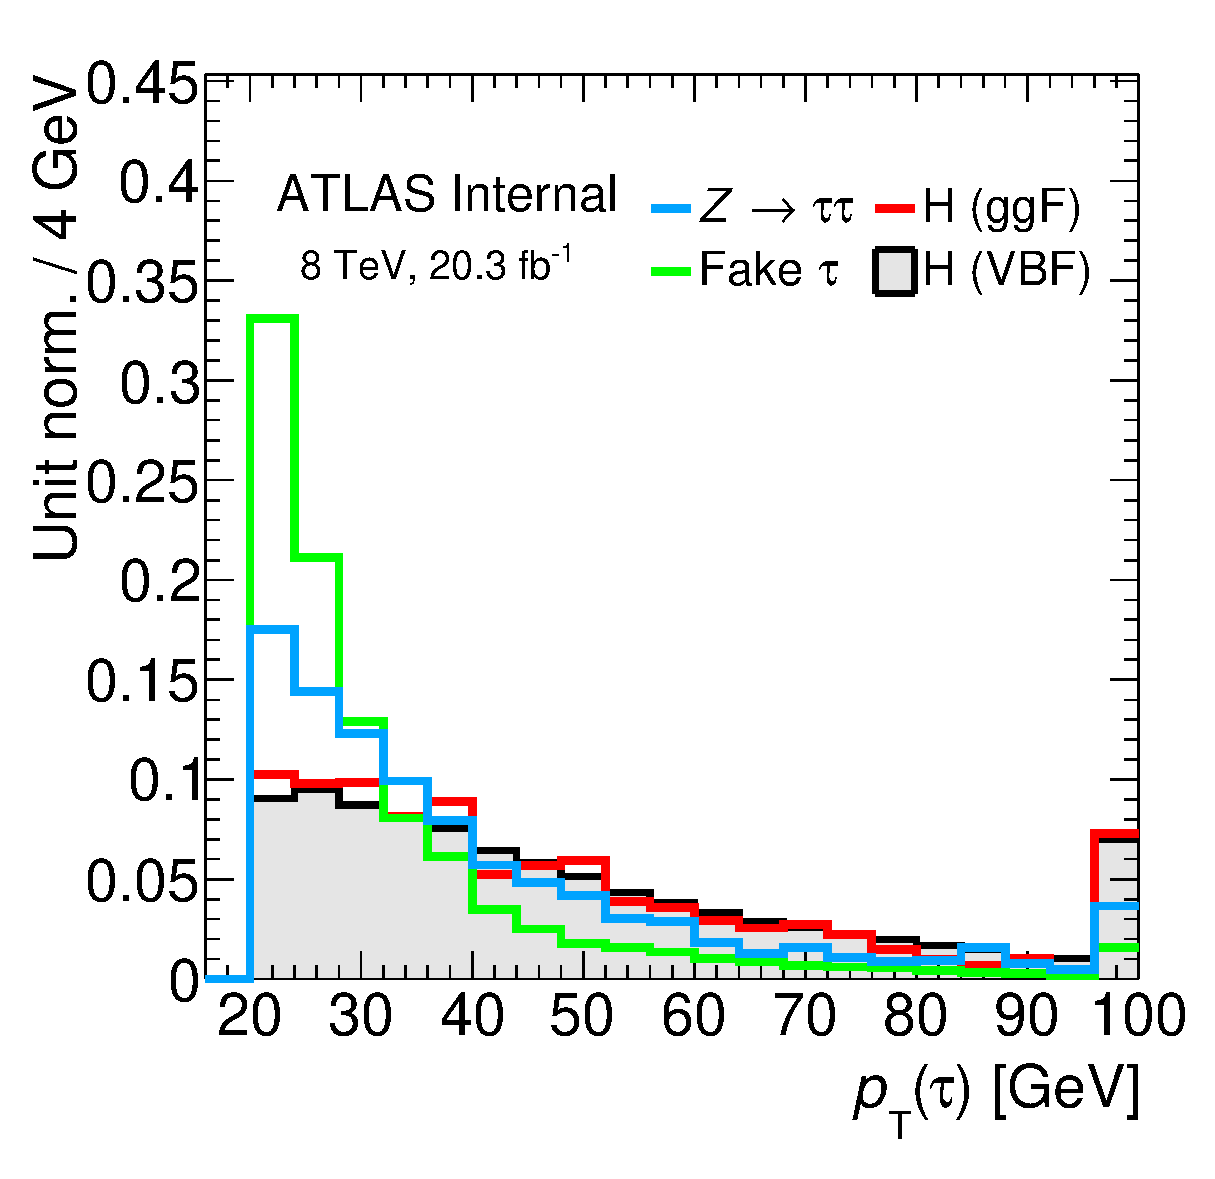
\includegraphics[width=0.35\textwidth]{figures/overlaid/vbf/tau-pt}
  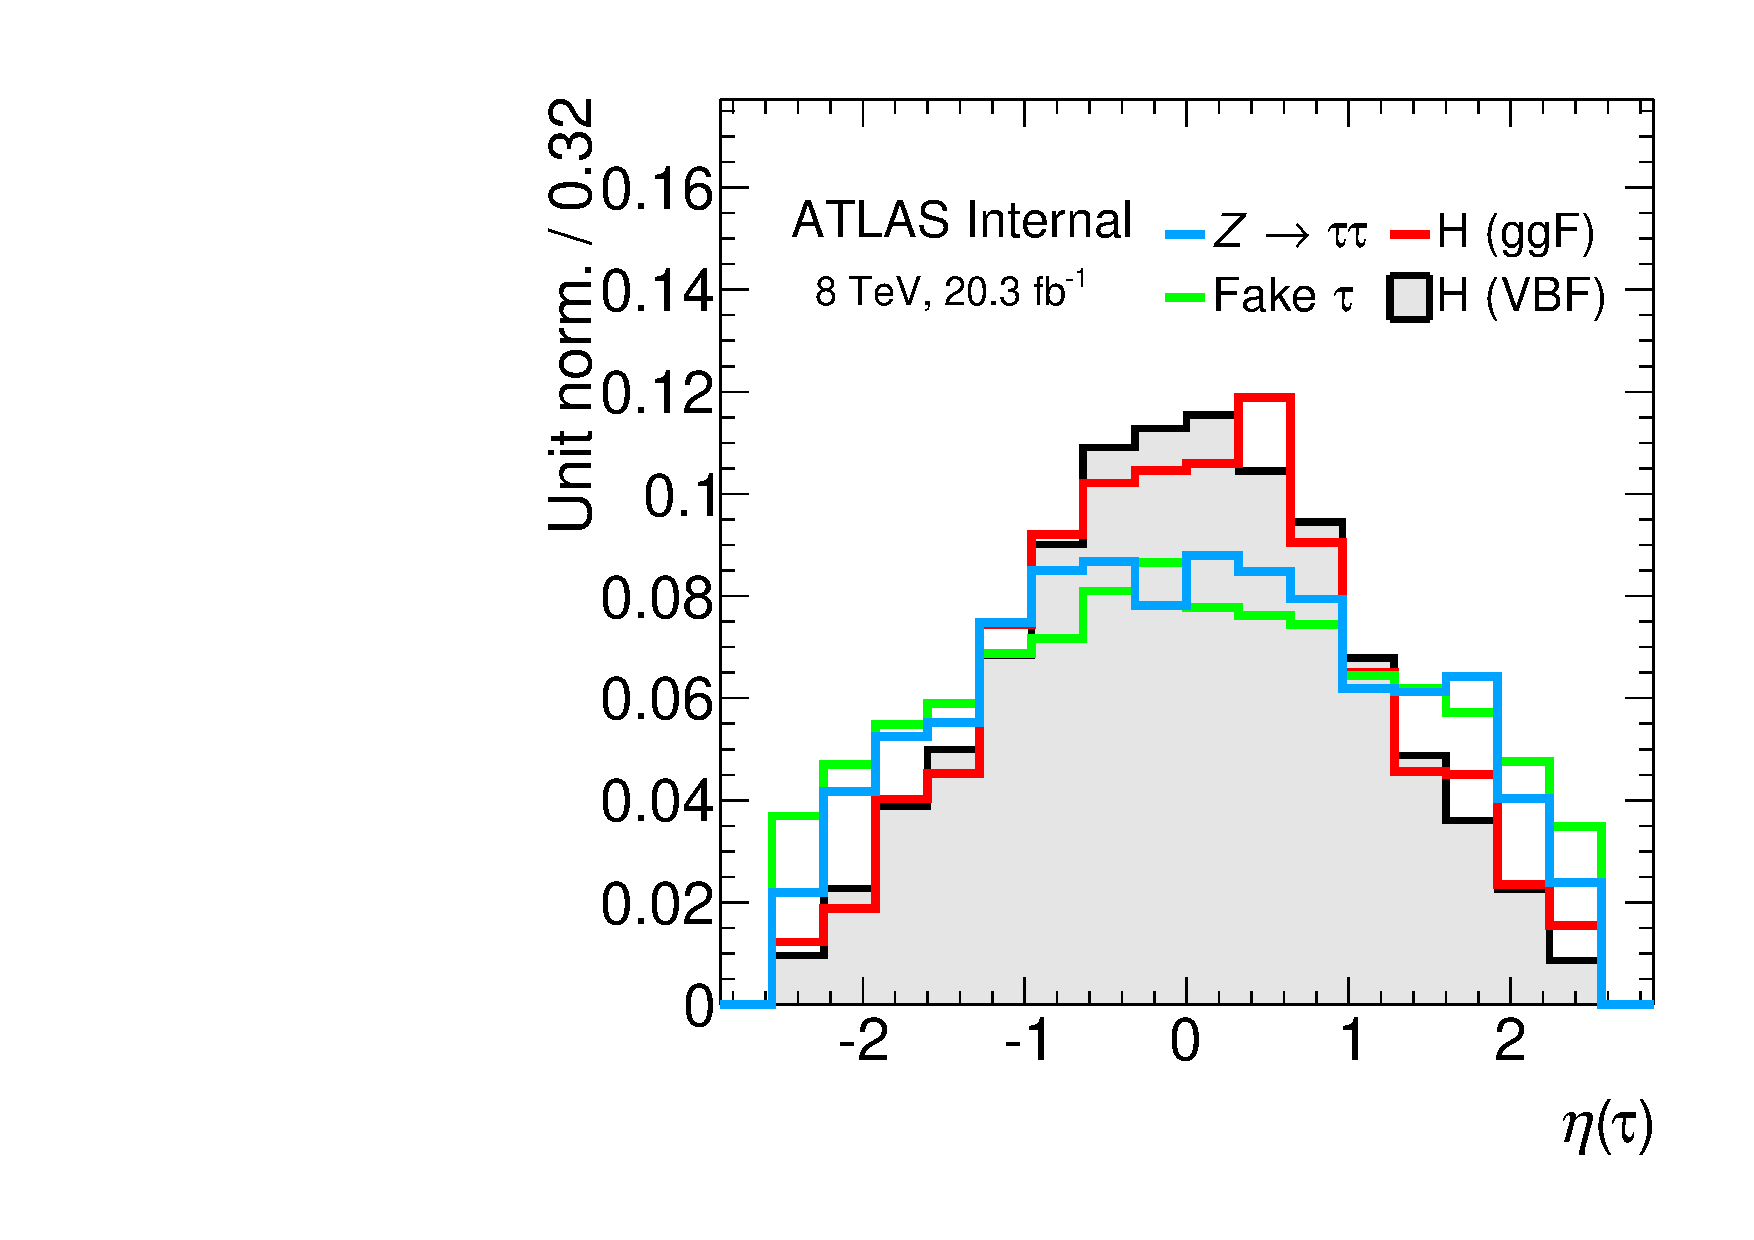
\includegraphics[width=0.35\textwidth]{figures/overlaid/vbf/tau-eta}
  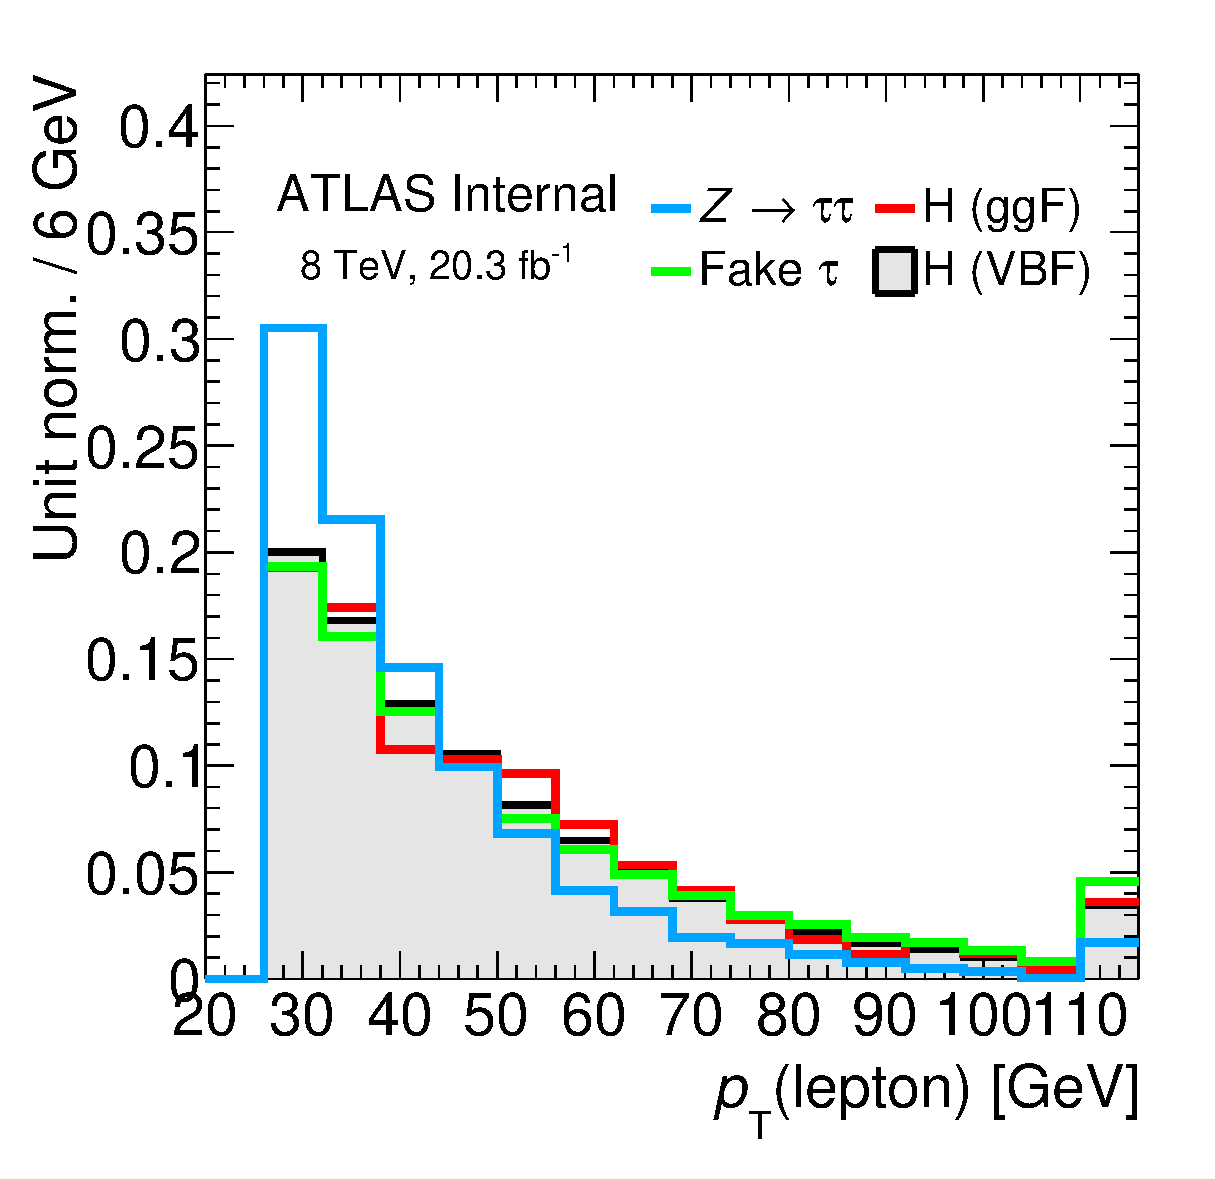
\includegraphics[width=0.35\textwidth]{figures/overlaid/vbf/lep-pt-hi}
  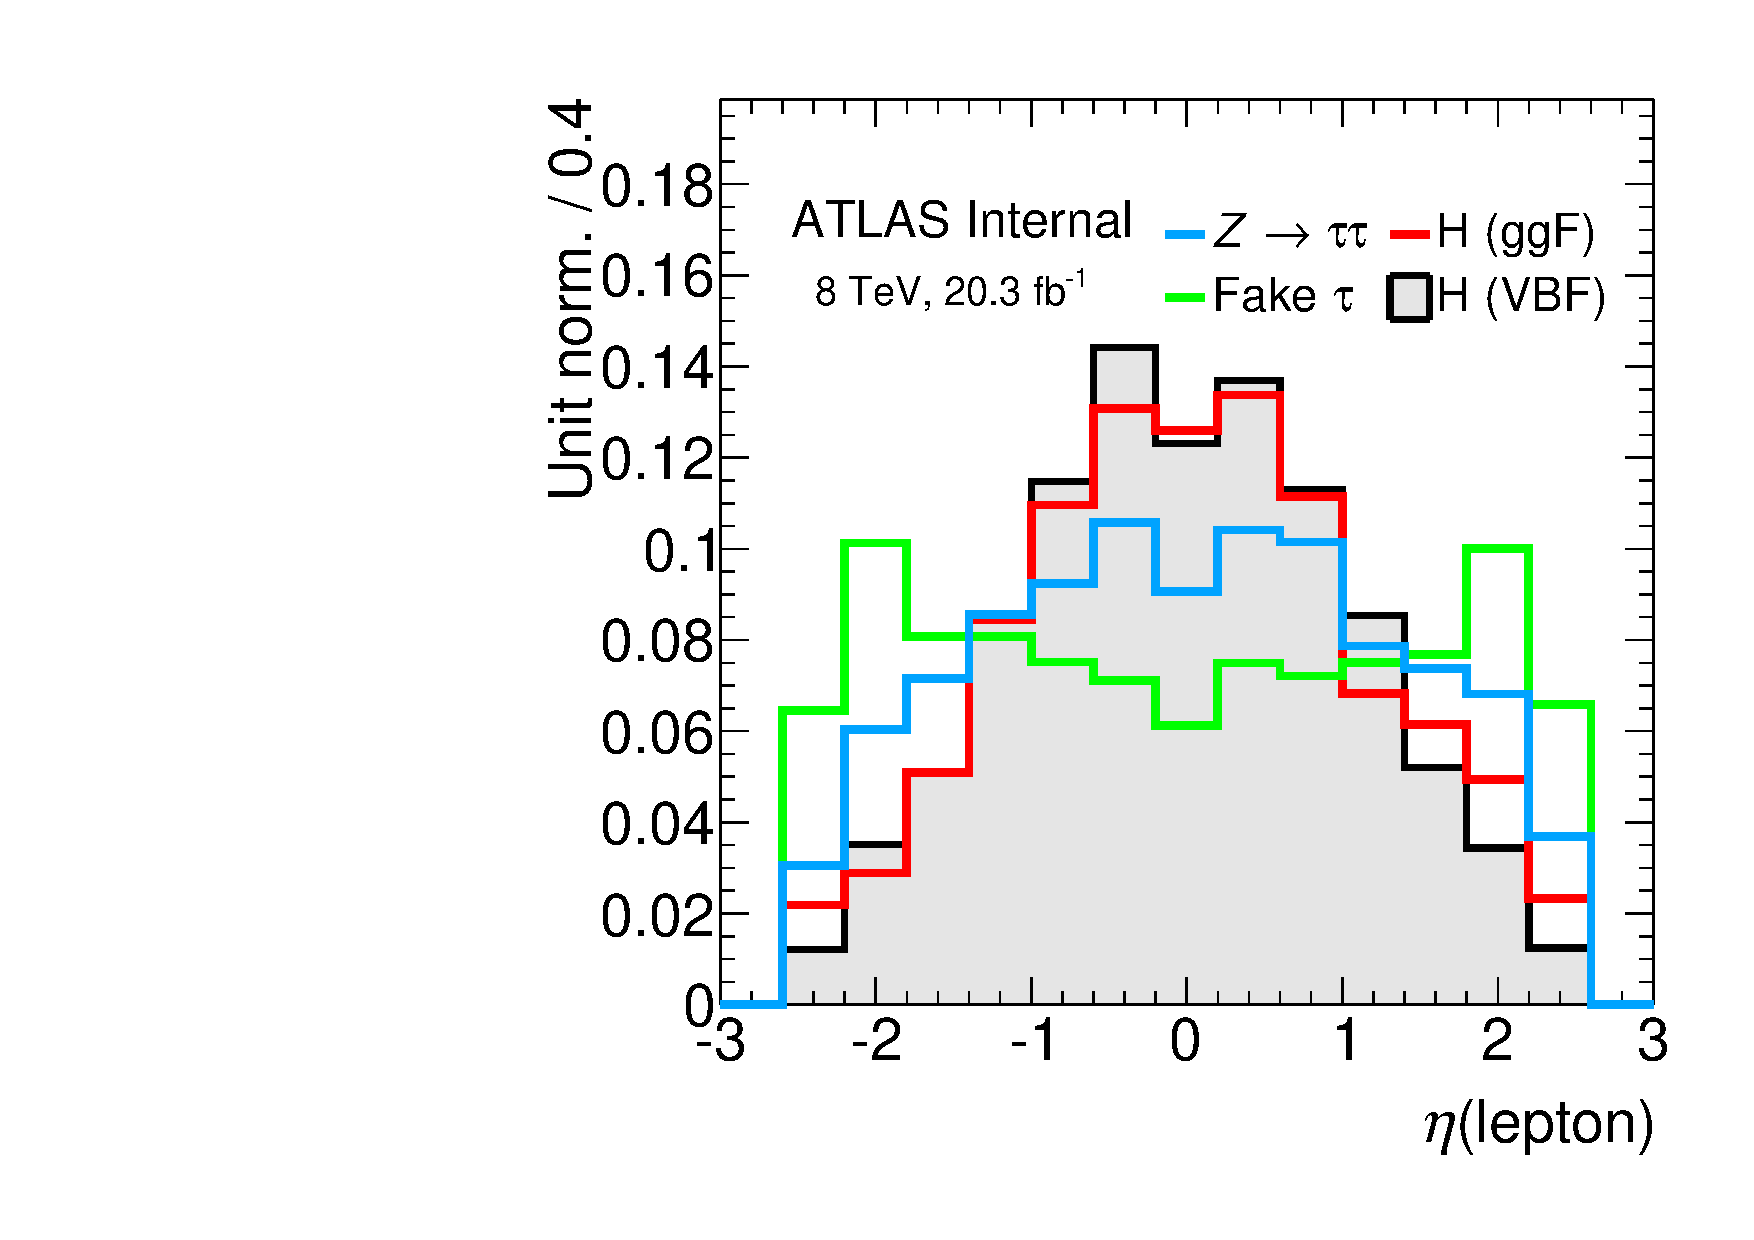
\includegraphics[width=0.35\textwidth]{figures/overlaid/vbf/lep-eta}
  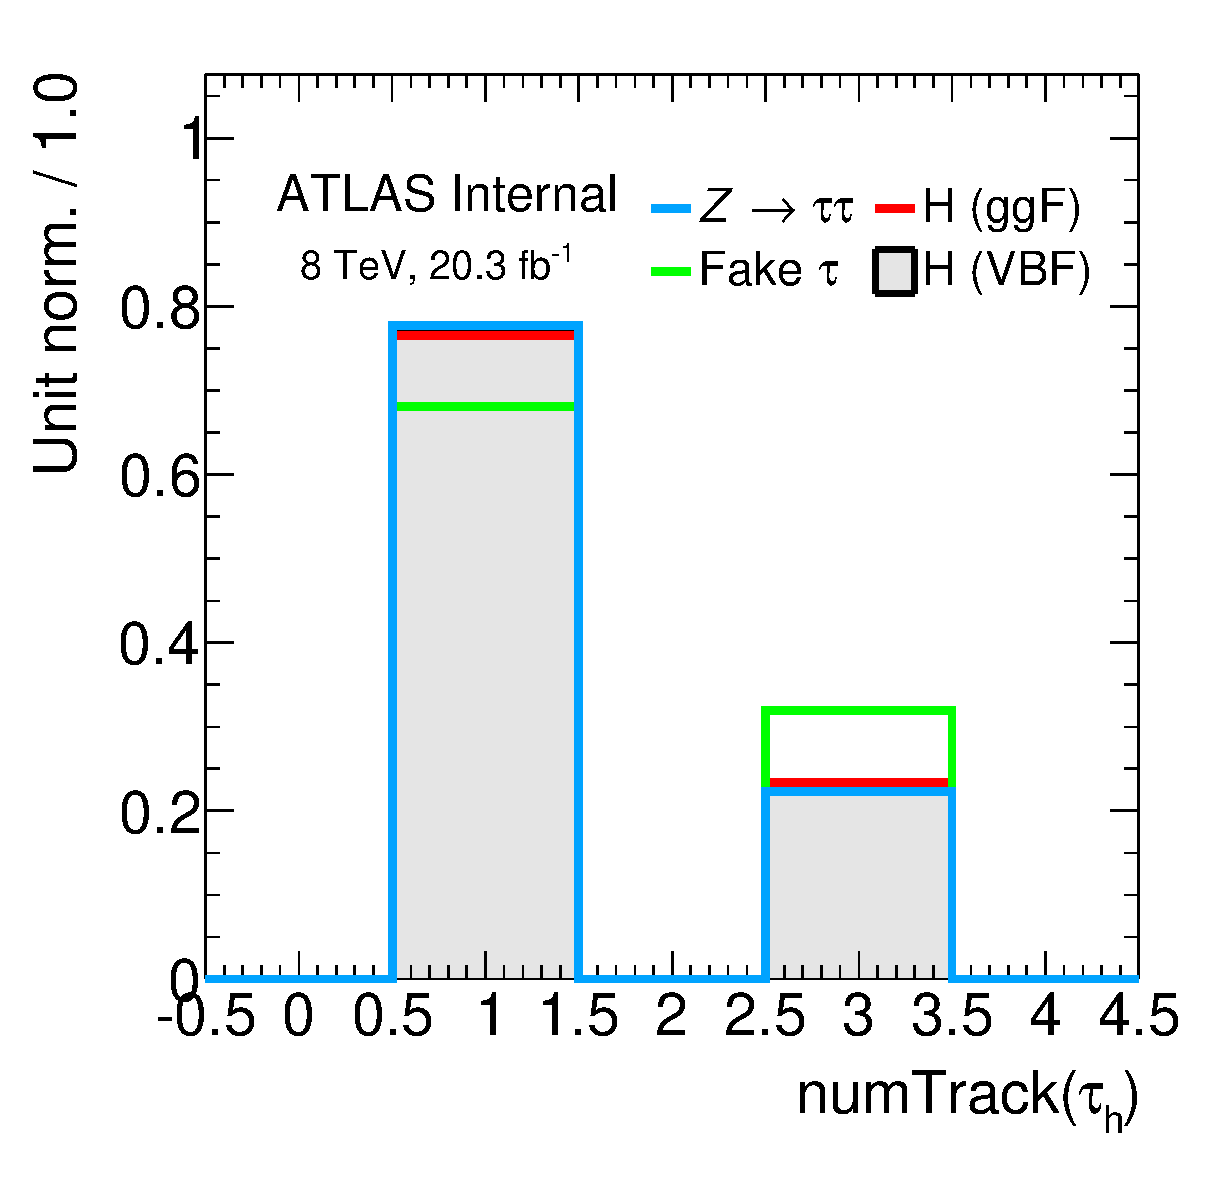
\includegraphics[width=0.35\textwidth]{figures/overlaid/vbf/tau-numTrack}
  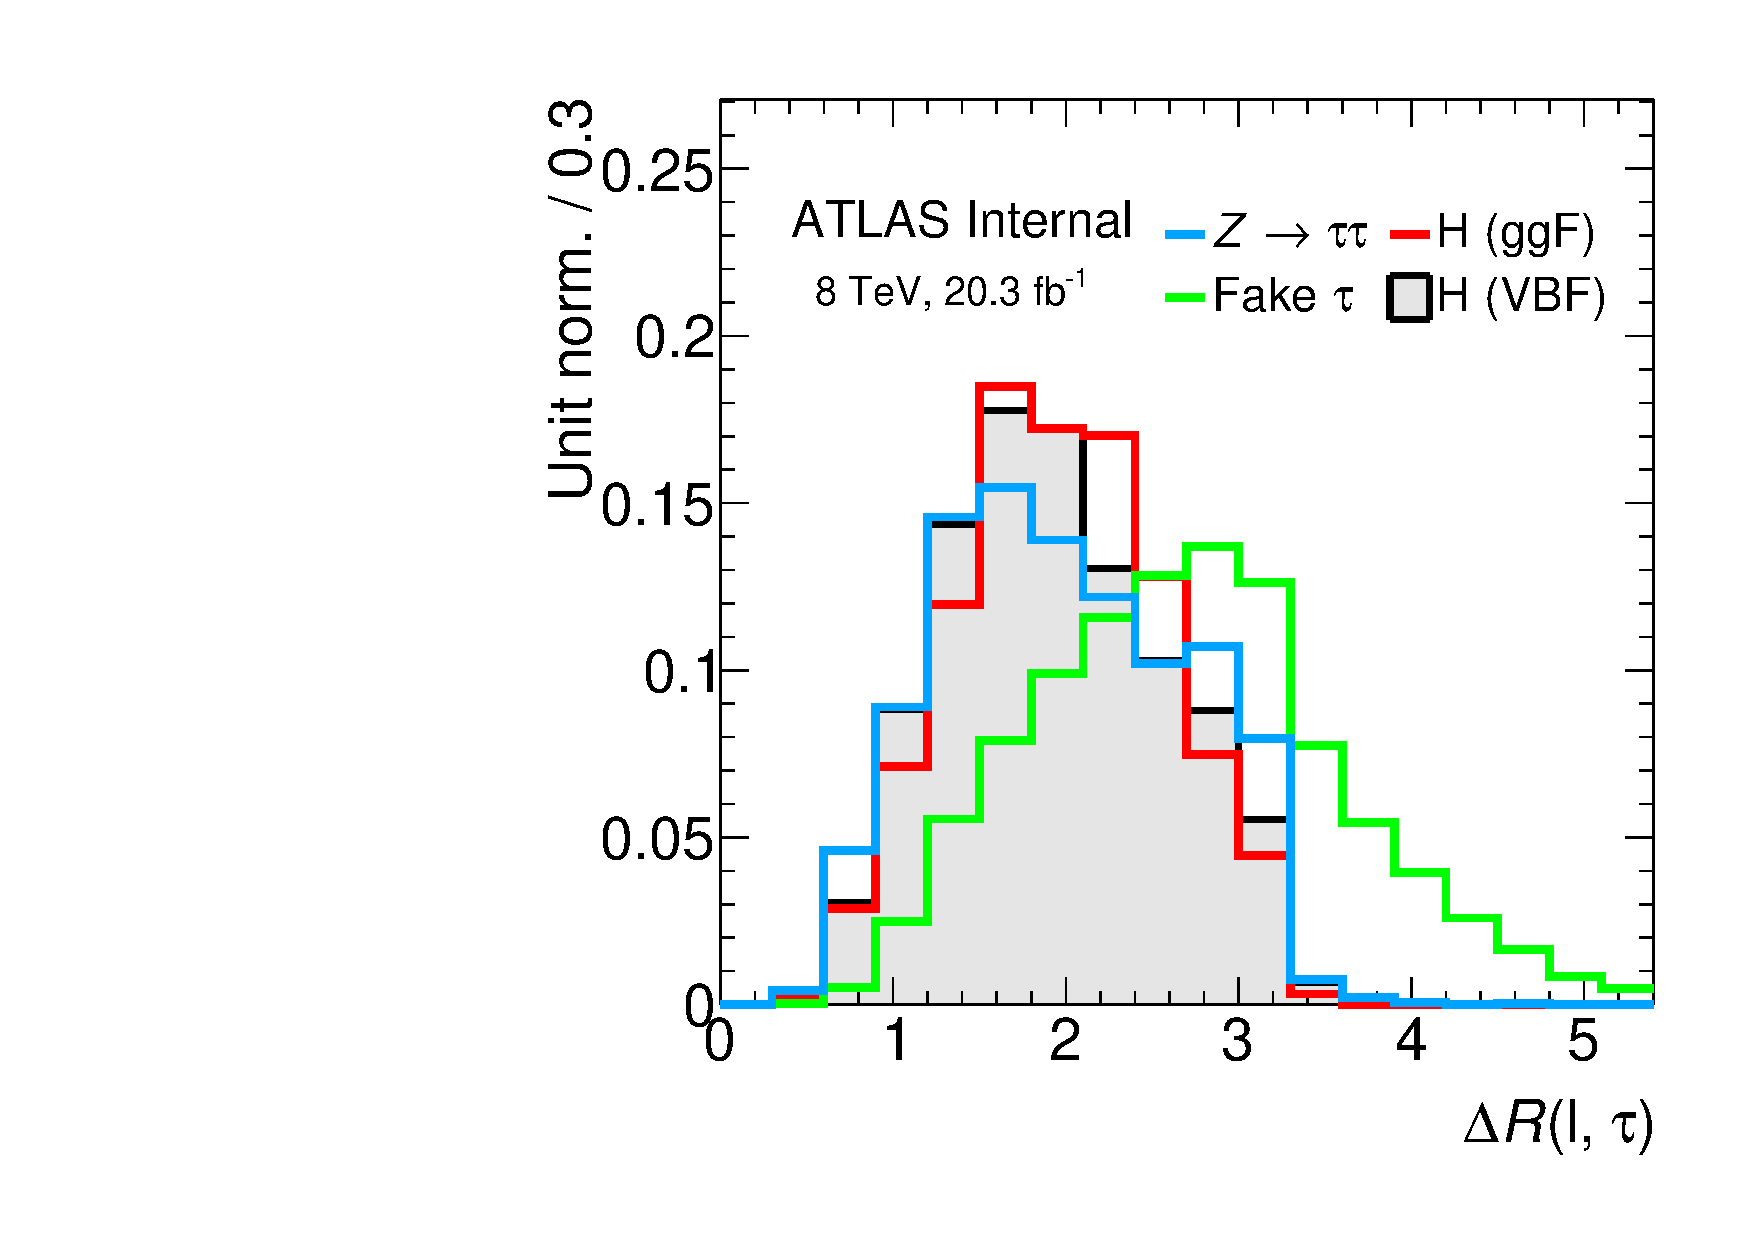
\includegraphics[width=0.35\textwidth]{figures/overlaid/vbf/taulep-dR}
  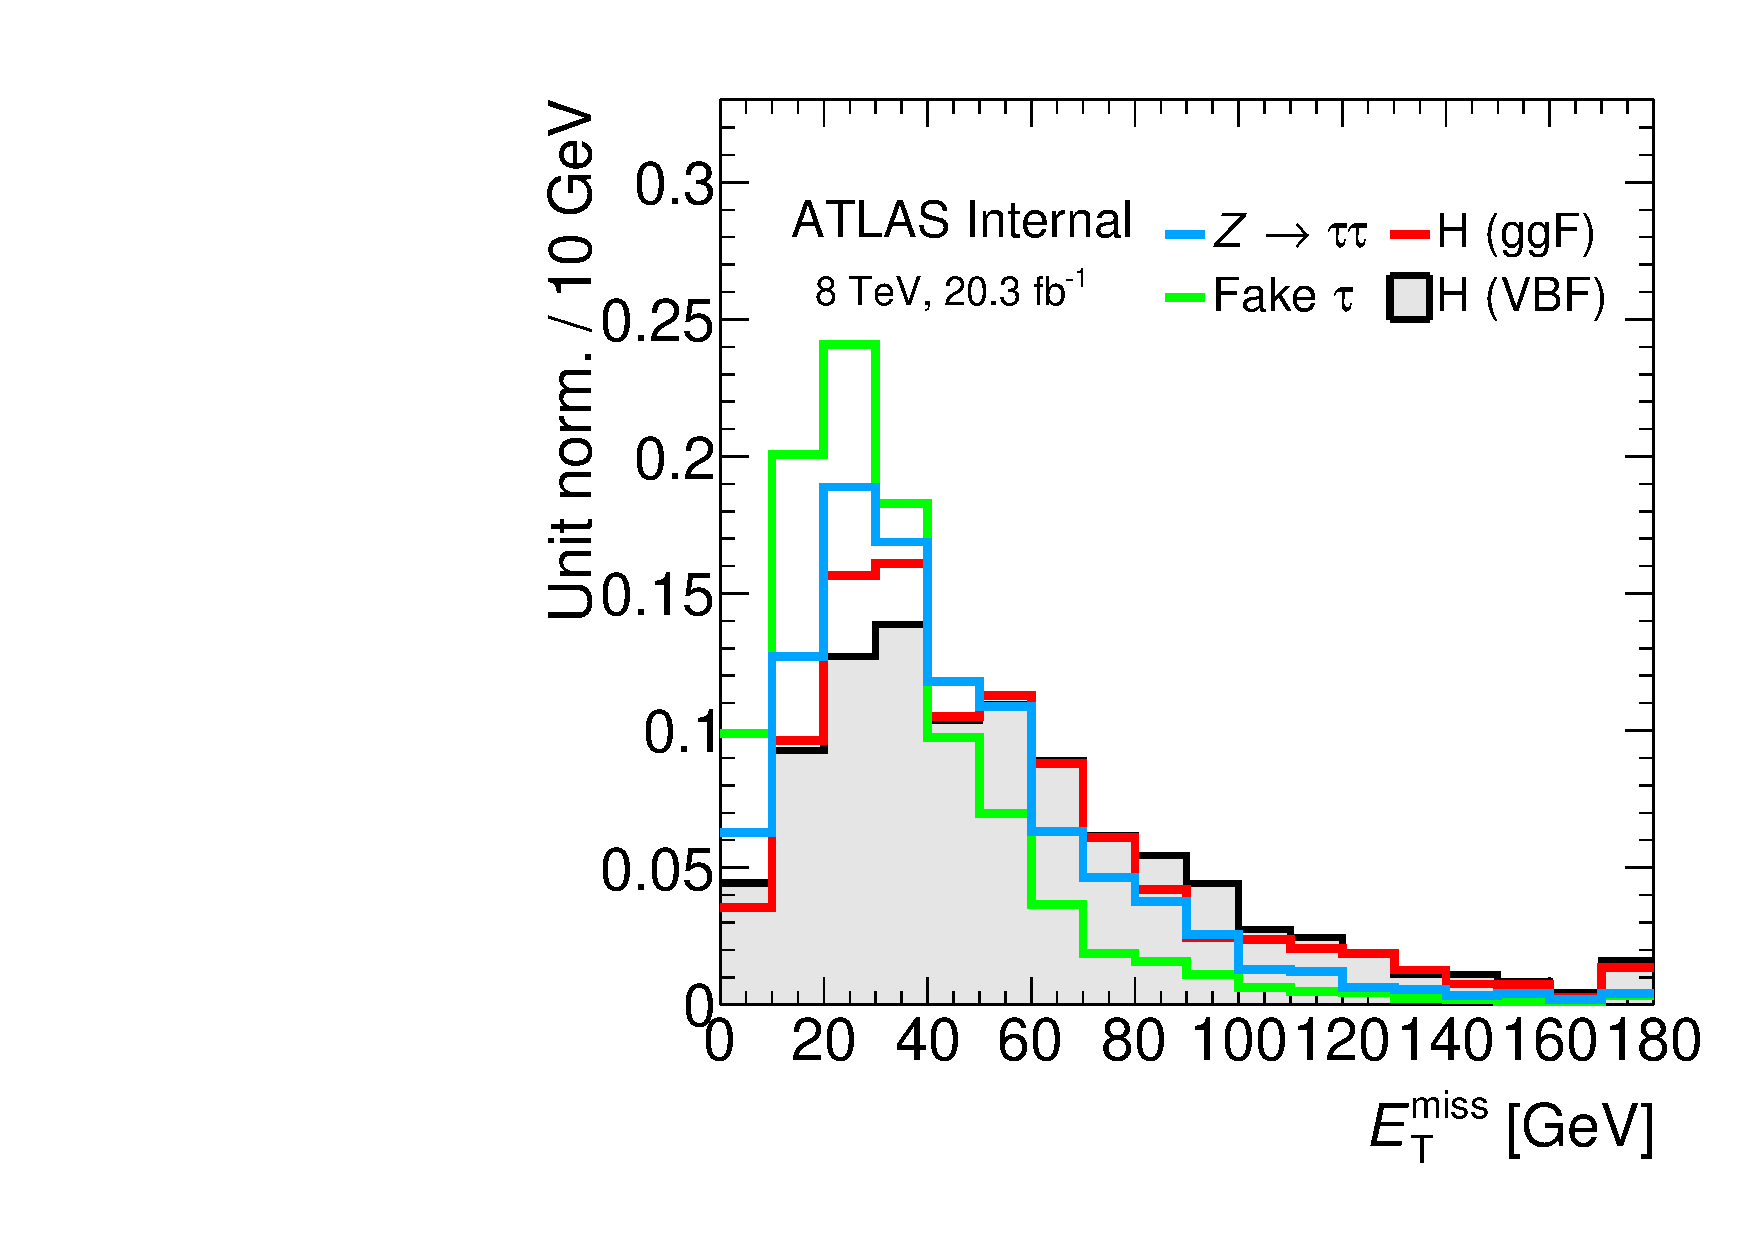
\includegraphics[width=0.35\textwidth]{figures/overlaid/vbf/met-pt-hi}
  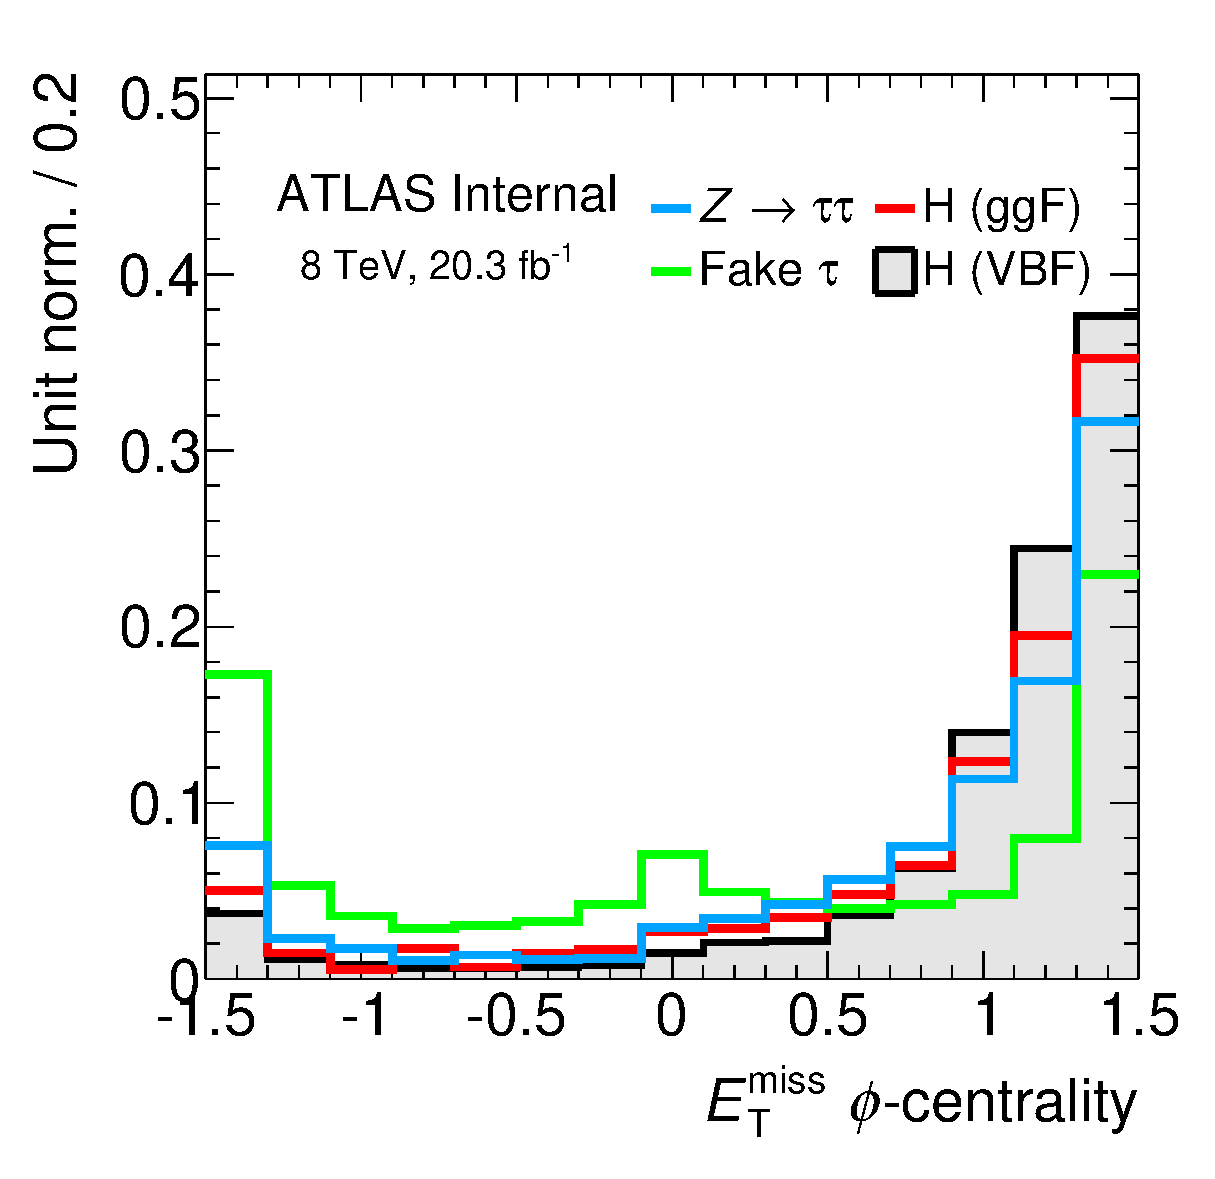
\includegraphics[width=0.35\textwidth]{figures/overlaid/vbf/met-phi-centrality}
  \caption{Variables.}
  \label{fig:strategy-overlaid-vbf-taus}
\end{figure}
\begin{figure}[tp]
  \centering
  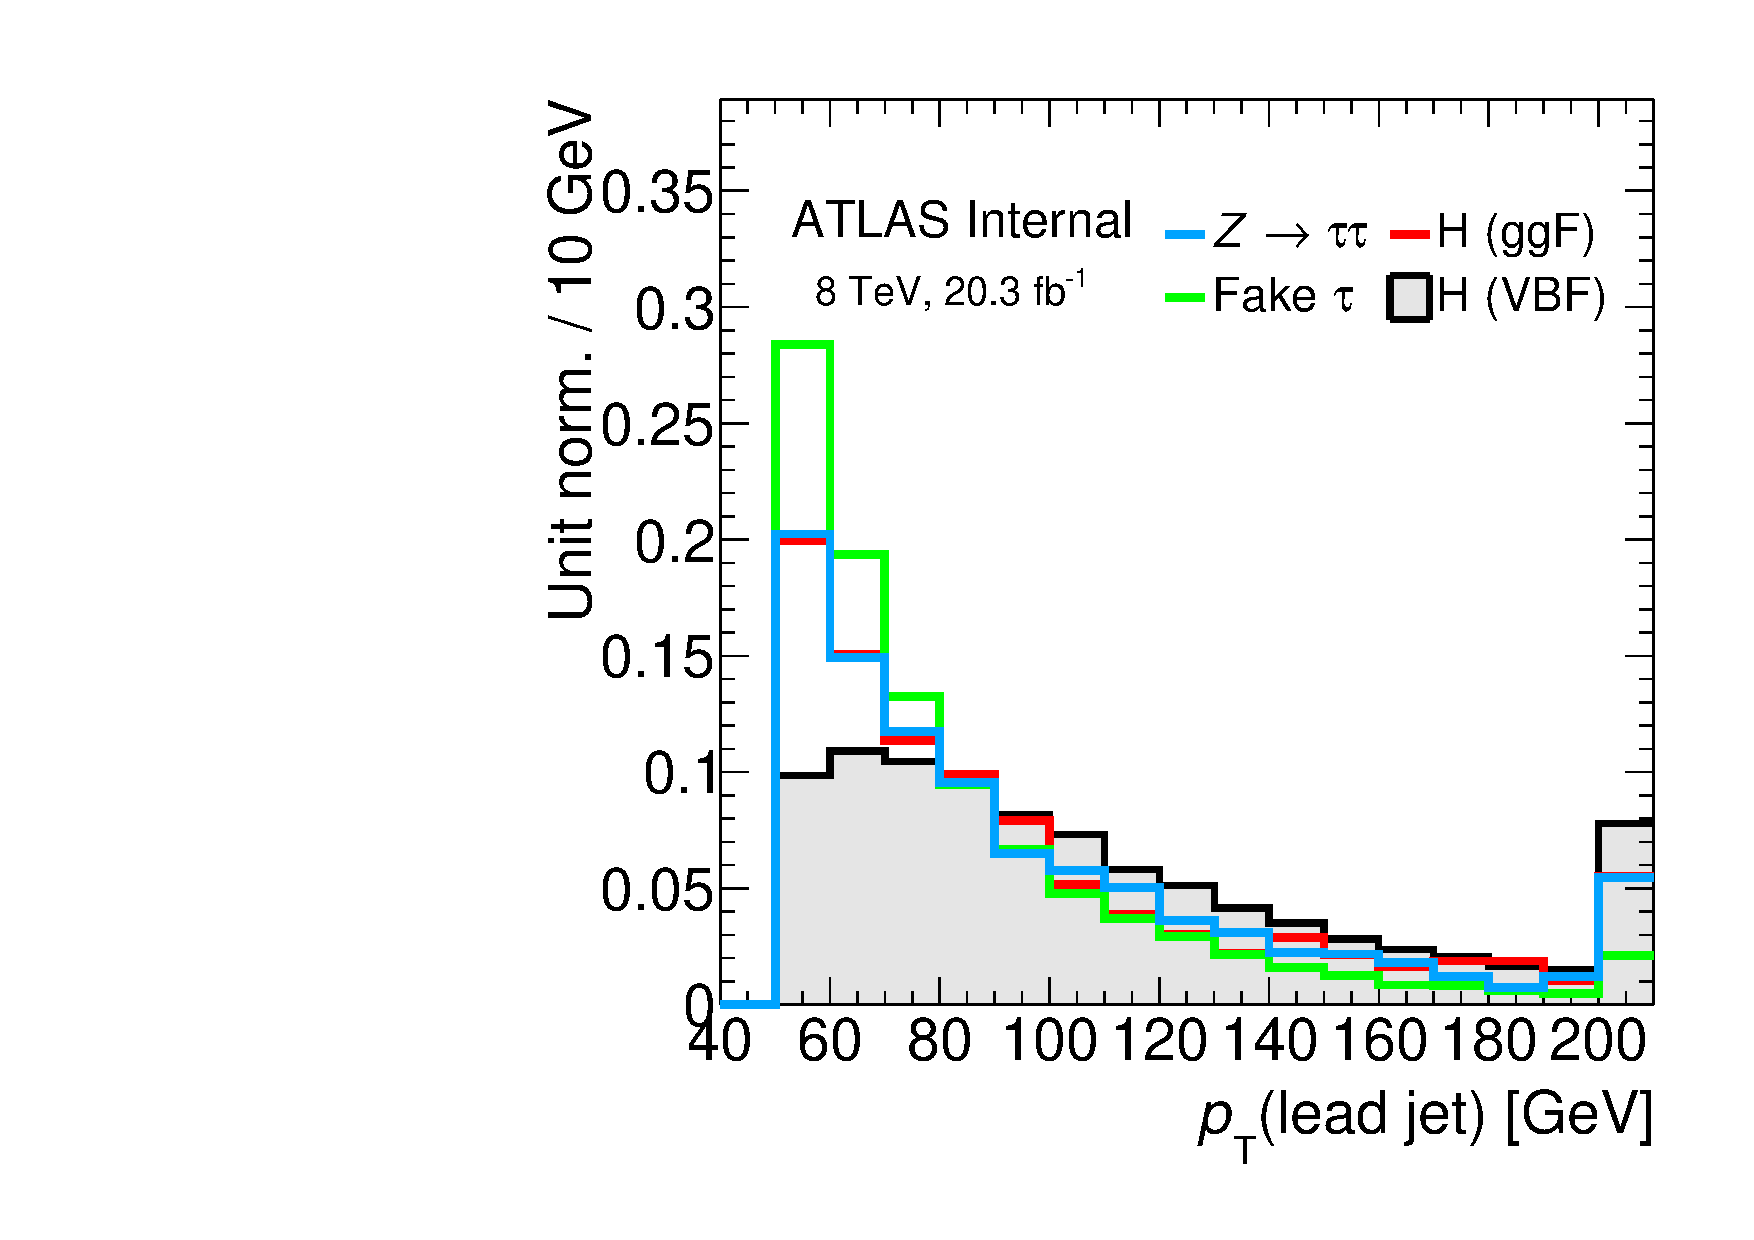
\includegraphics[width=0.35\textwidth]{figures/overlaid/vbf/jet-1-pt}
  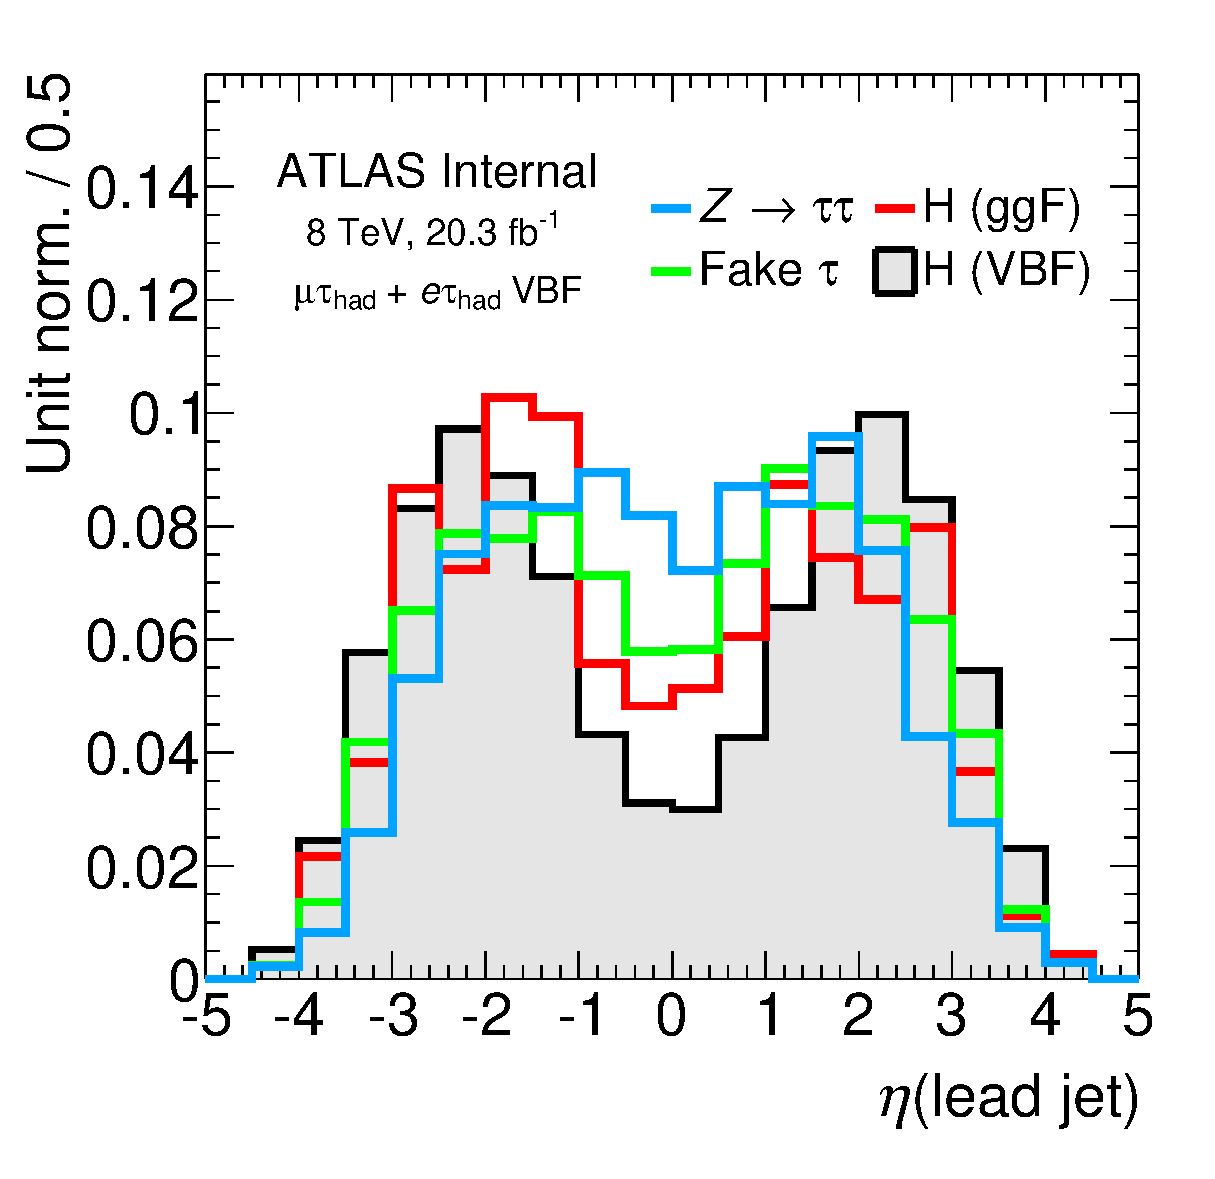
\includegraphics[width=0.35\textwidth]{figures/overlaid/vbf/jet-1-eta}
  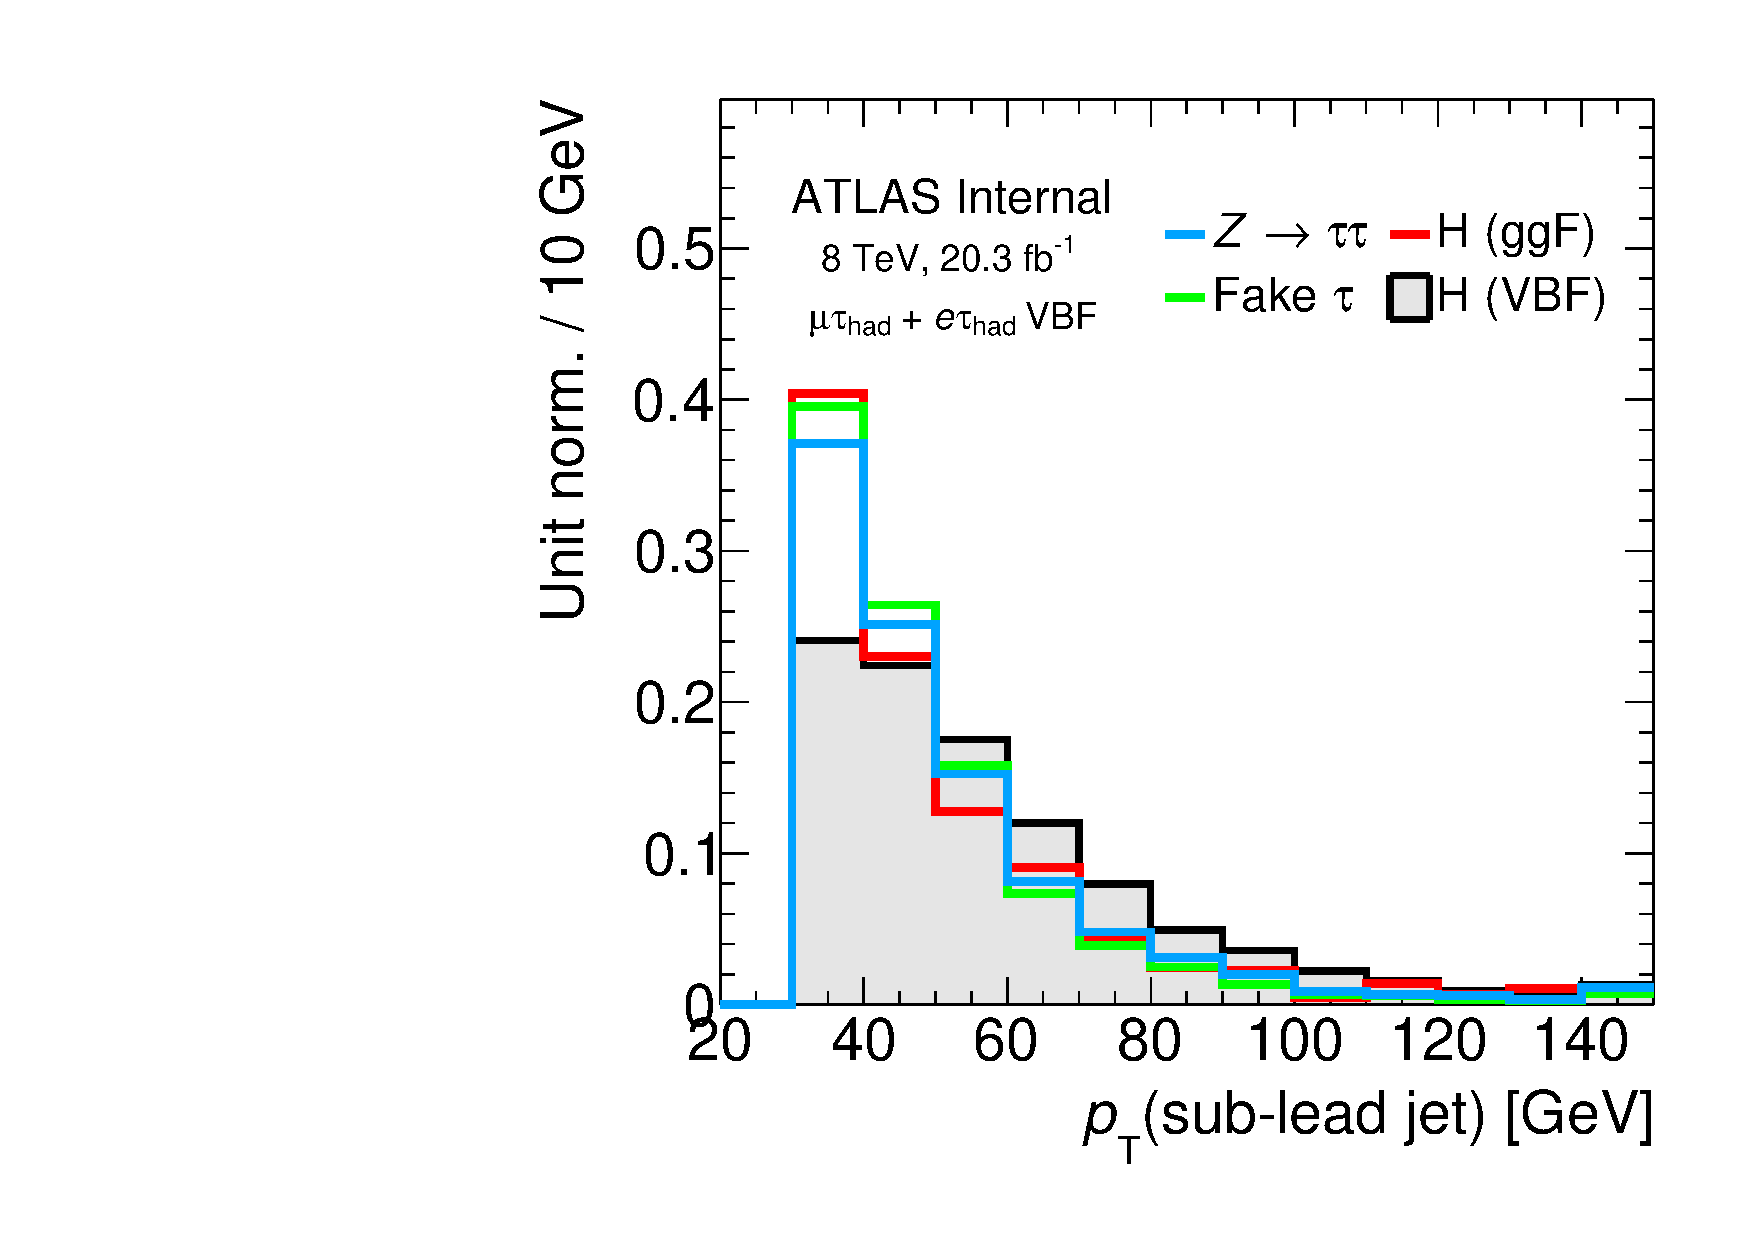
\includegraphics[width=0.35\textwidth]{figures/overlaid/vbf/jet-2-pt}
  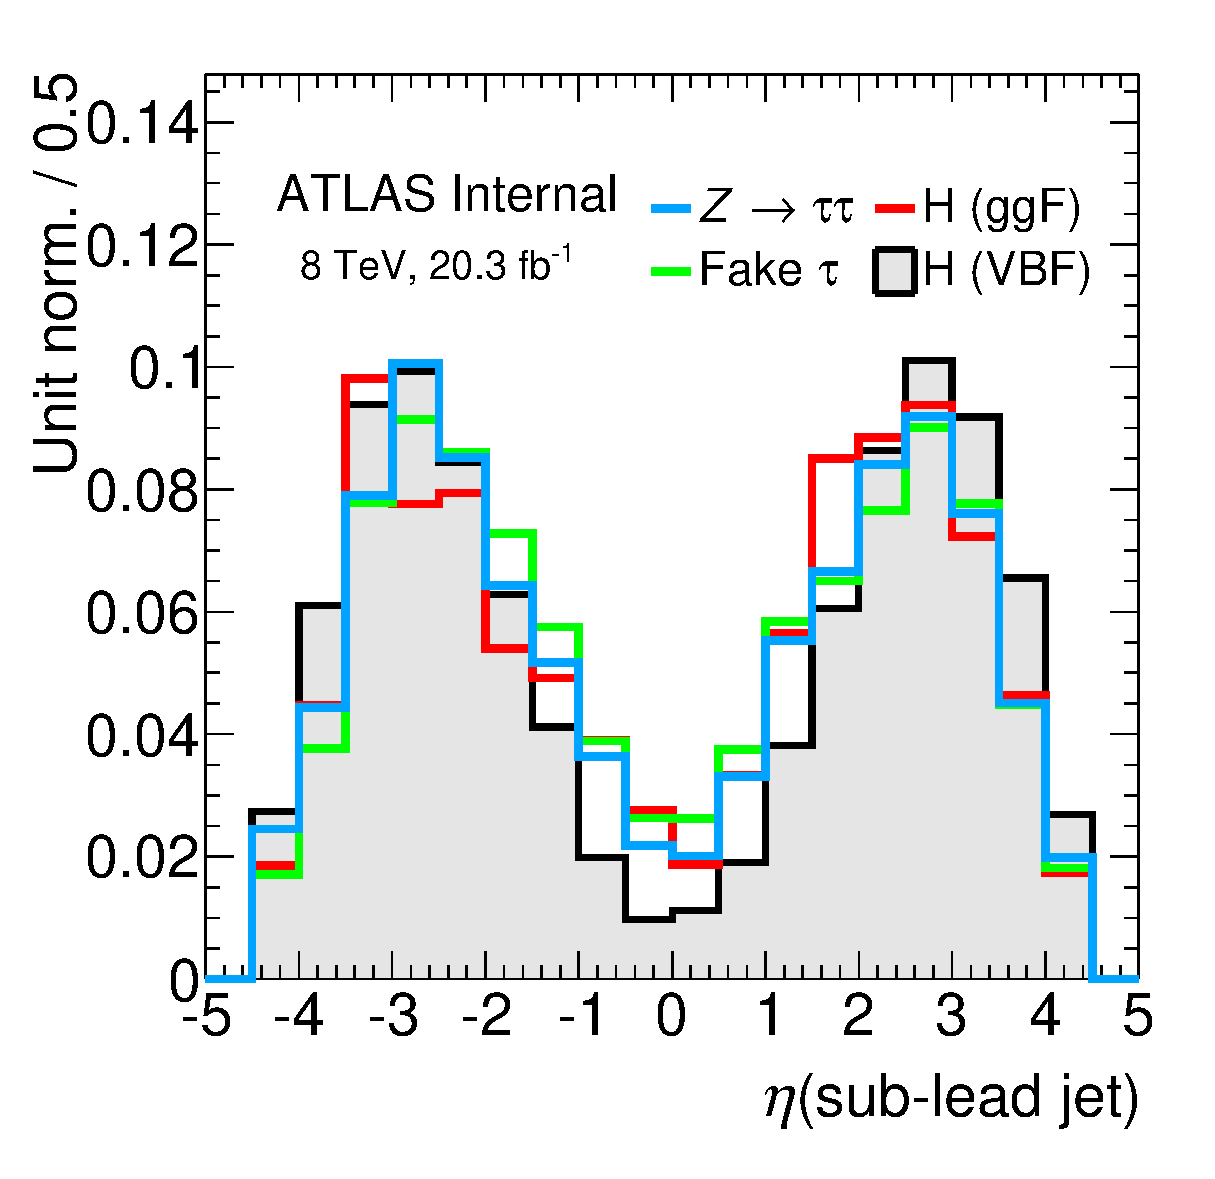
\includegraphics[width=0.35\textwidth]{figures/overlaid/vbf/jet-2-eta}
  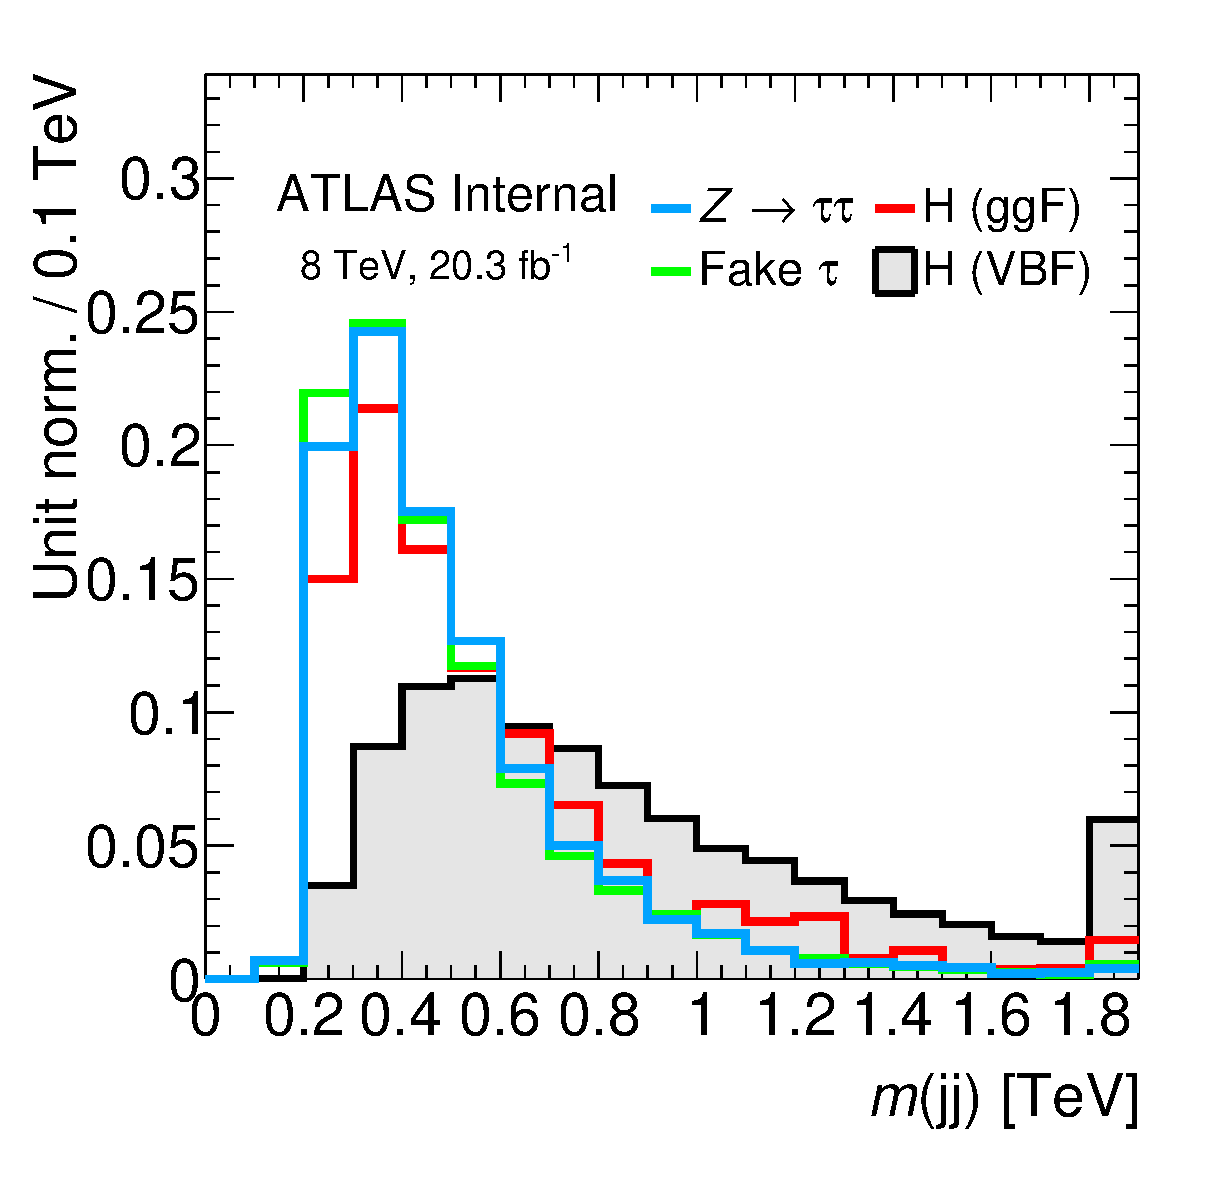
\includegraphics[width=0.35\textwidth]{figures/overlaid/vbf/dijet-m-veryhigh}
  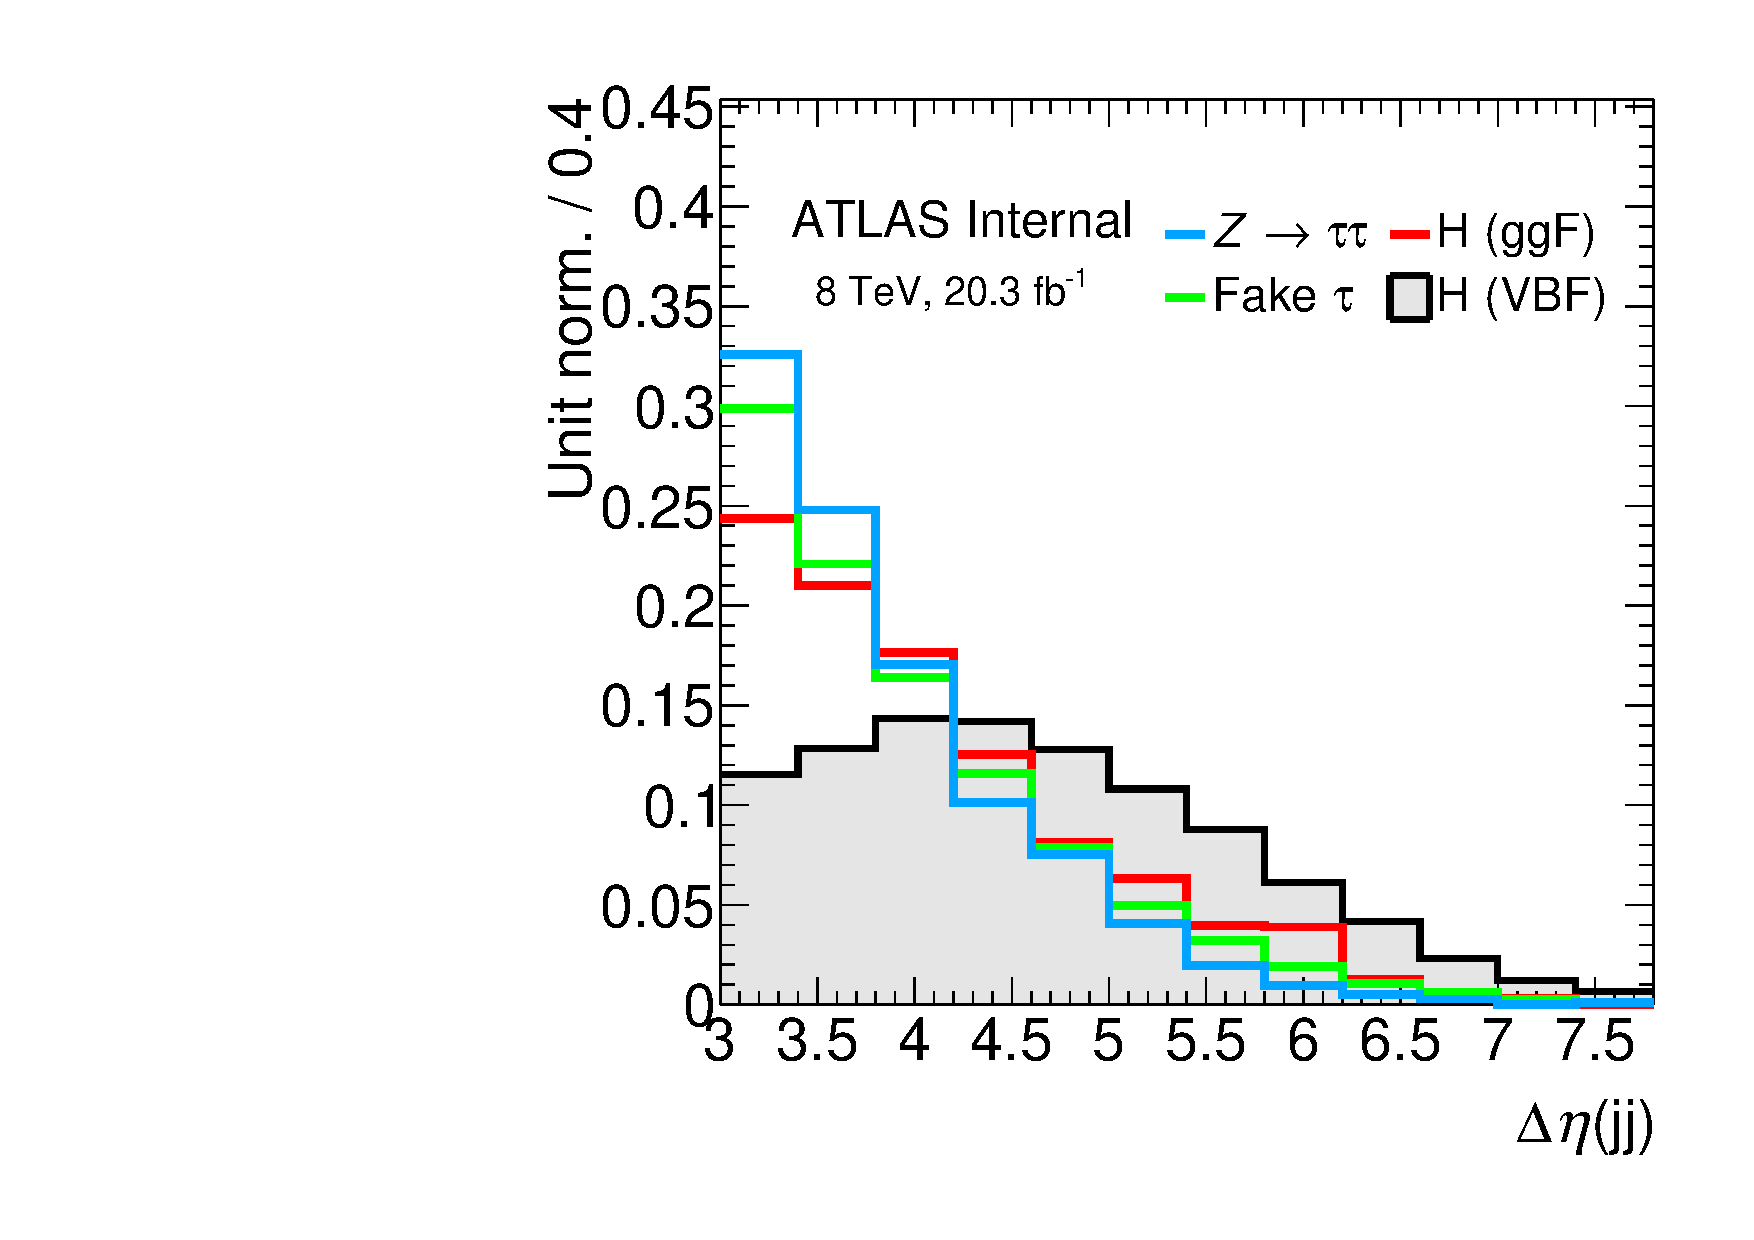
\includegraphics[width=0.35\textwidth]{figures/overlaid/vbf/jets-deta}
  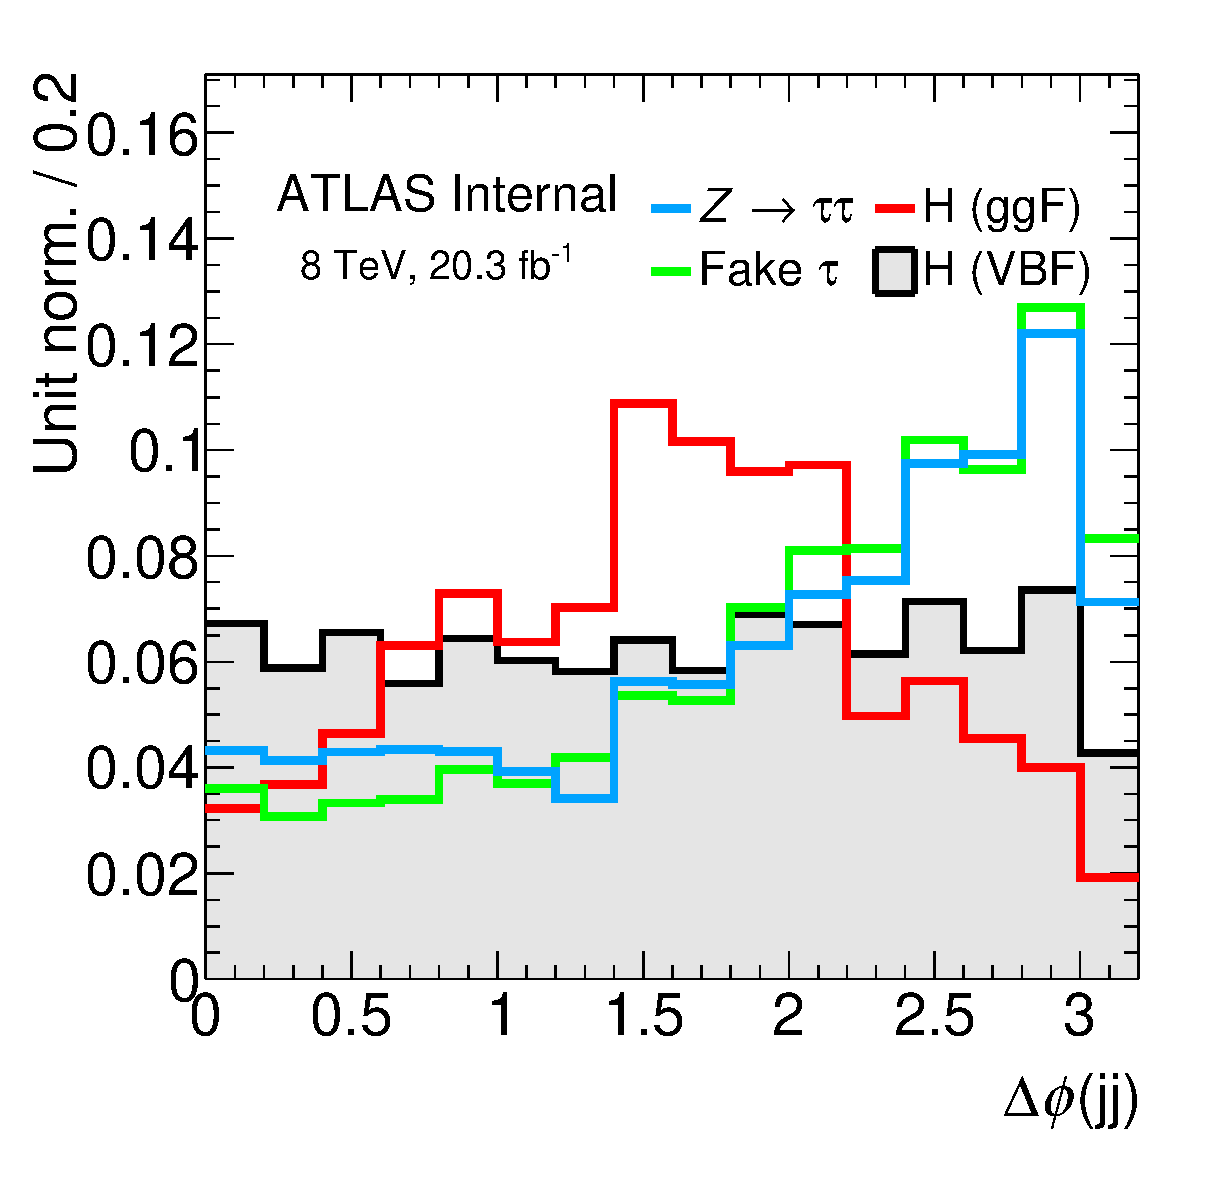
\includegraphics[width=0.35\textwidth]{figures/overlaid/vbf/jets-dphi}
  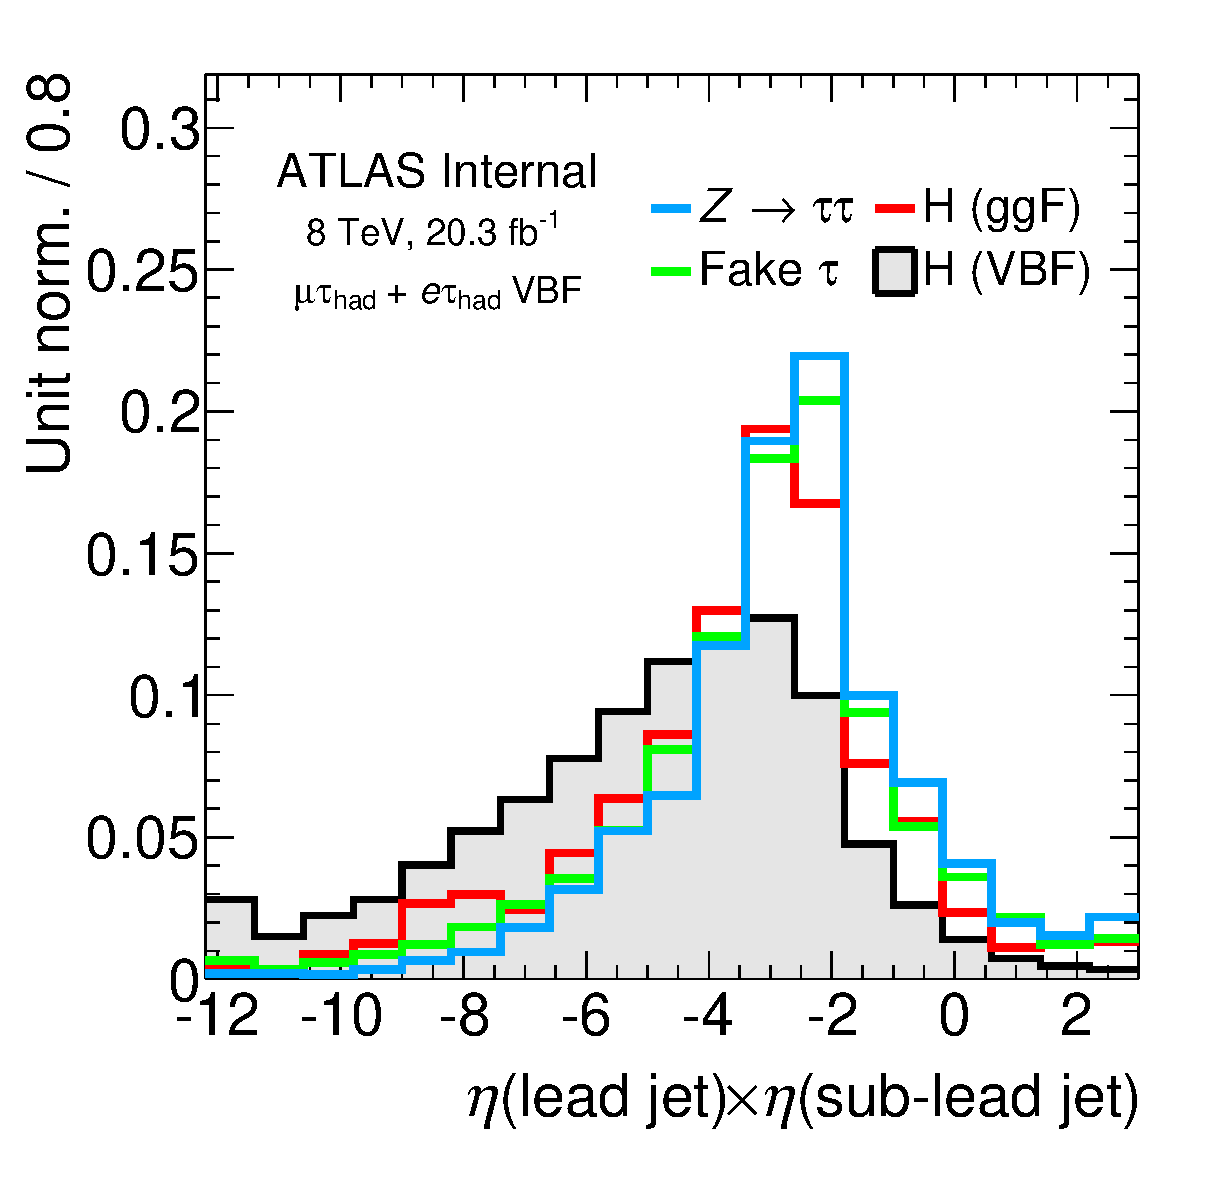
\includegraphics[width=0.35\textwidth]{figures/overlaid/vbf/jets-etaprod}
  \caption{Variables.}
  \label{fig:strategy-overlaid-vbf-jets}
\end{figure}
\begin{figure}[tp]
  \centering
  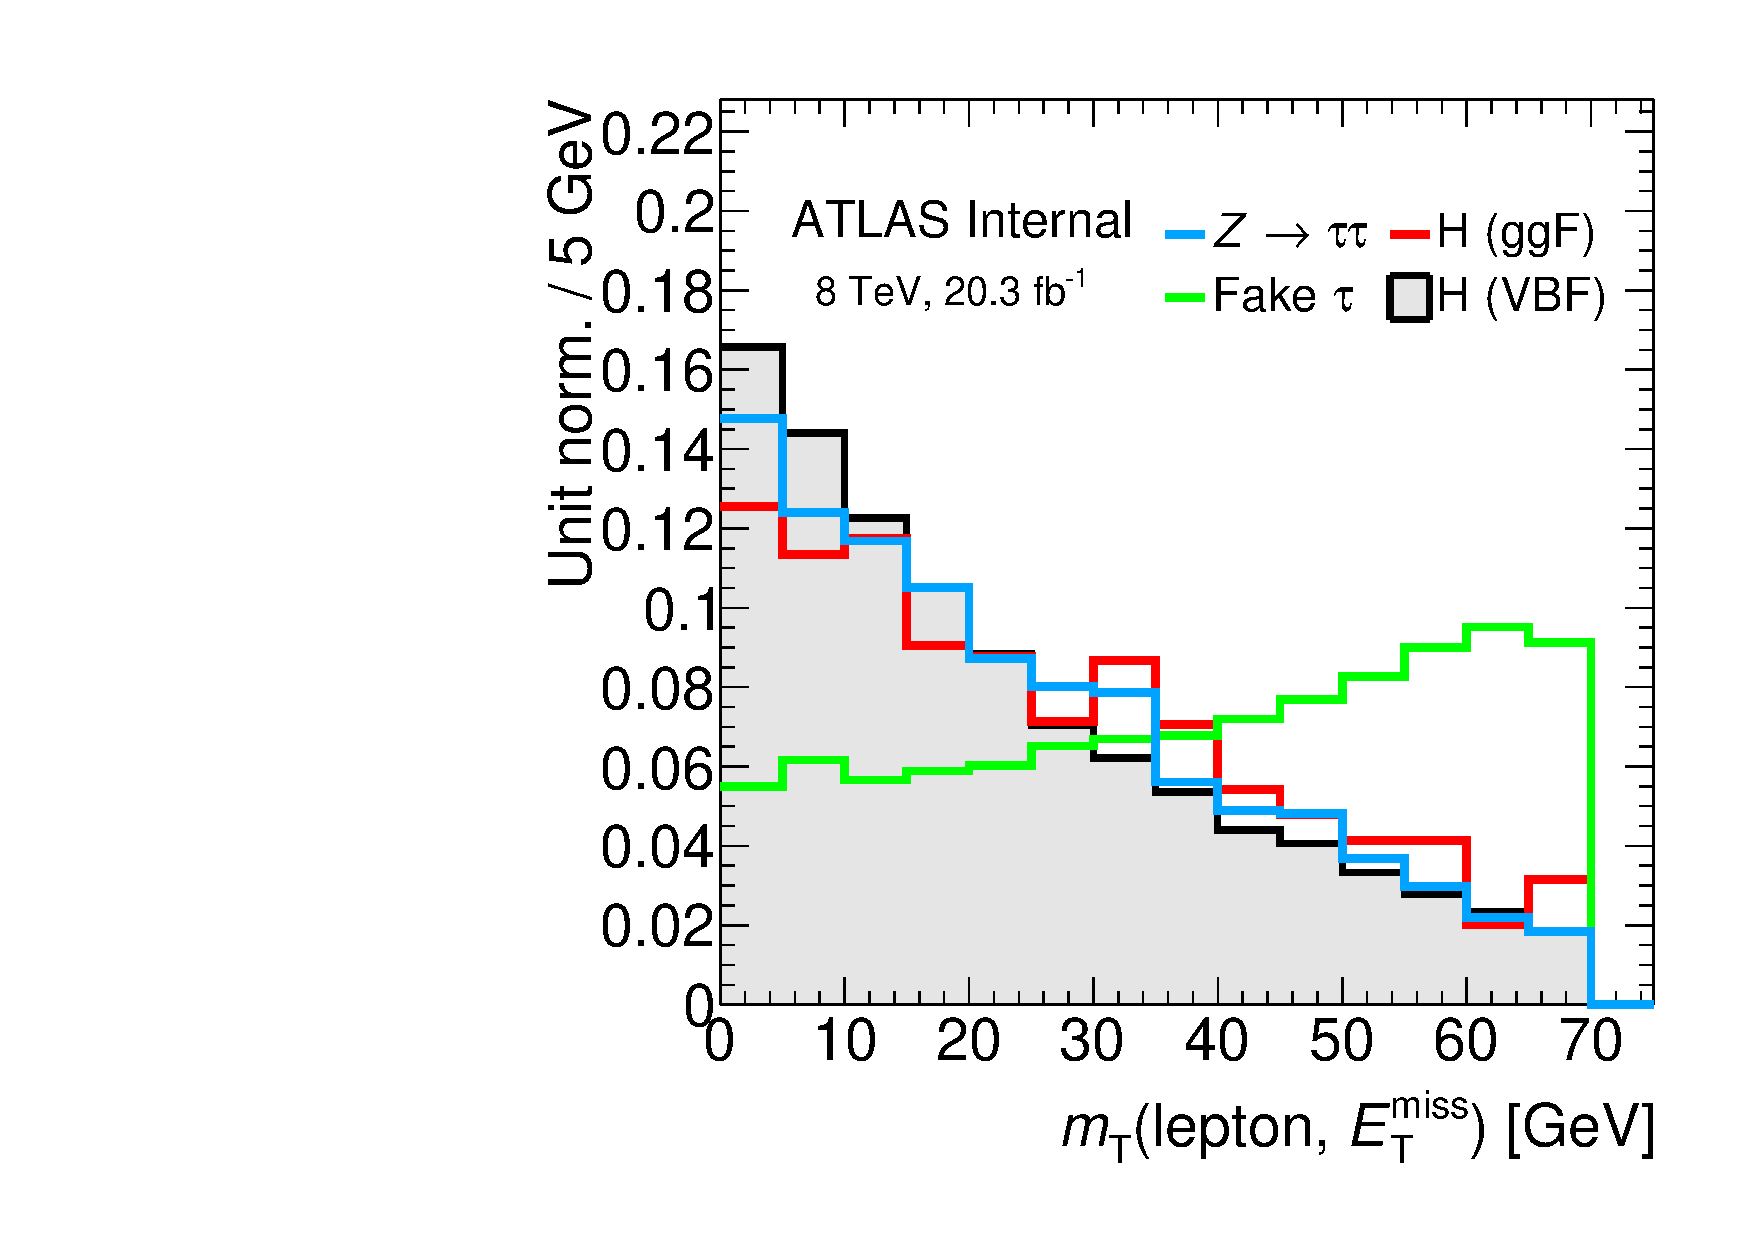
\includegraphics[width=0.45\textwidth]{figures/overlaid/vbf/mT}
  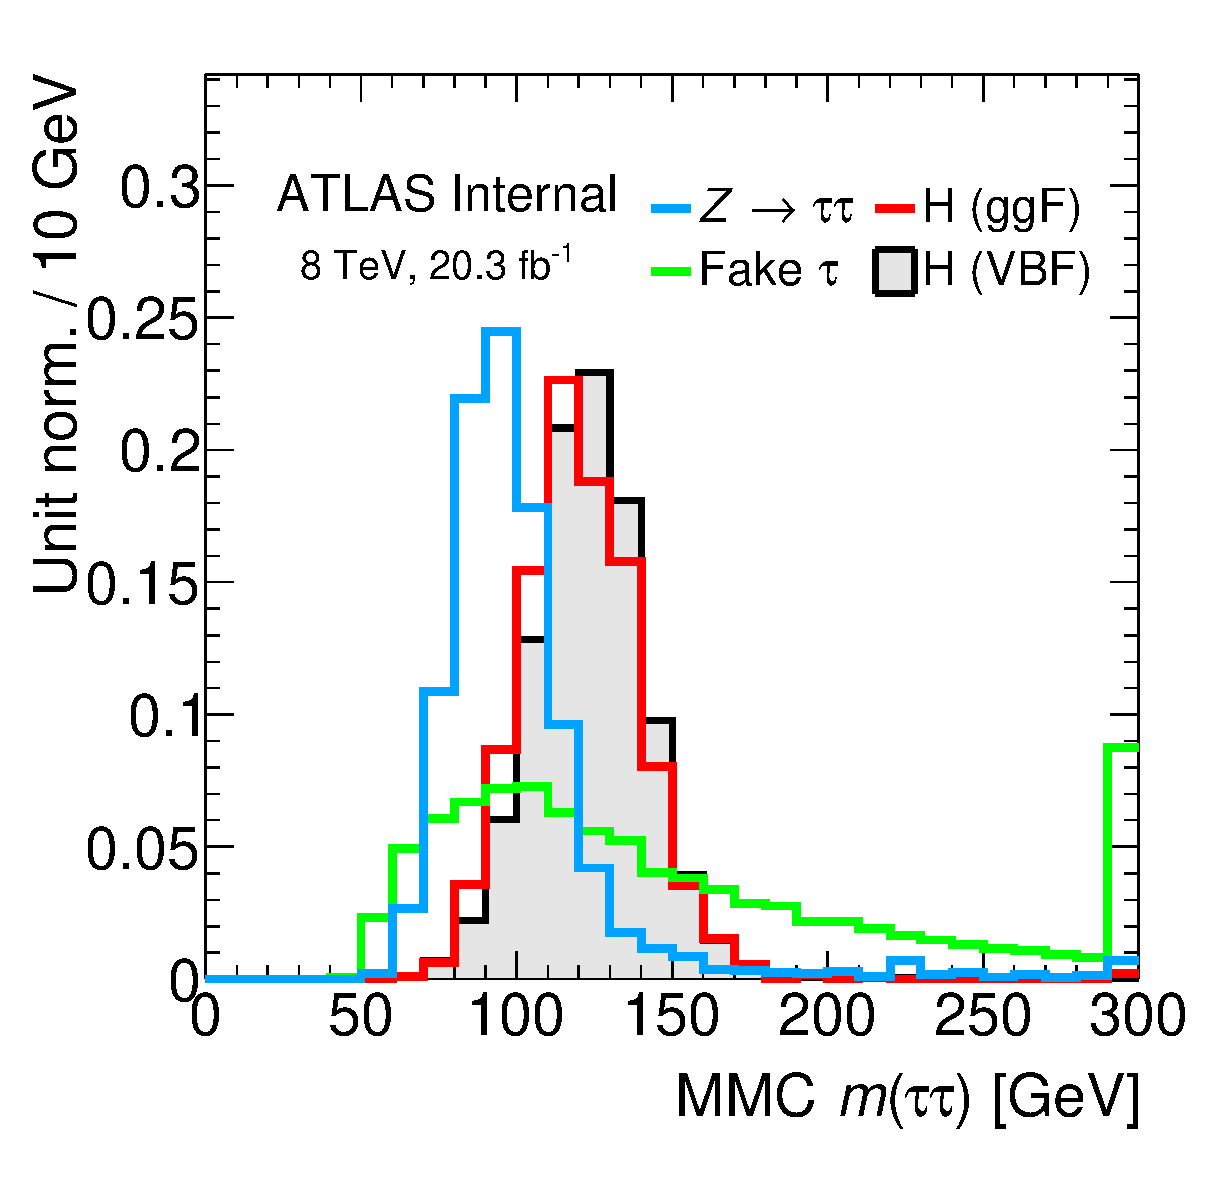
\includegraphics[width=0.45\textwidth]{figures/overlaid/vbf/mMMC}
  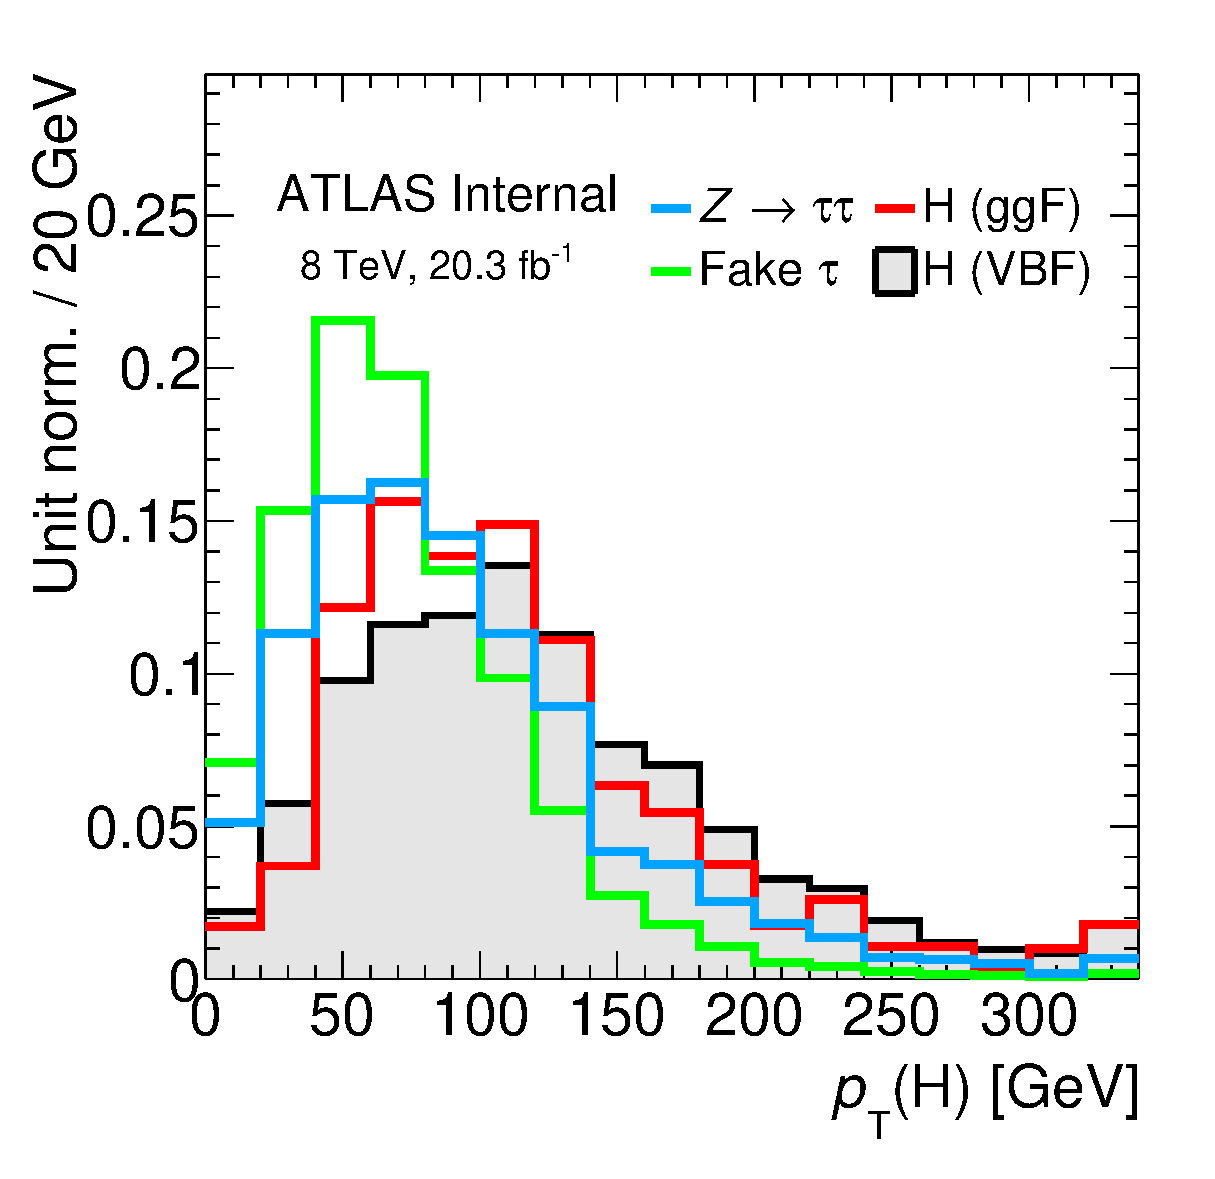
\includegraphics[width=0.45\textwidth]{figures/overlaid/vbf/H-pt-hi}
  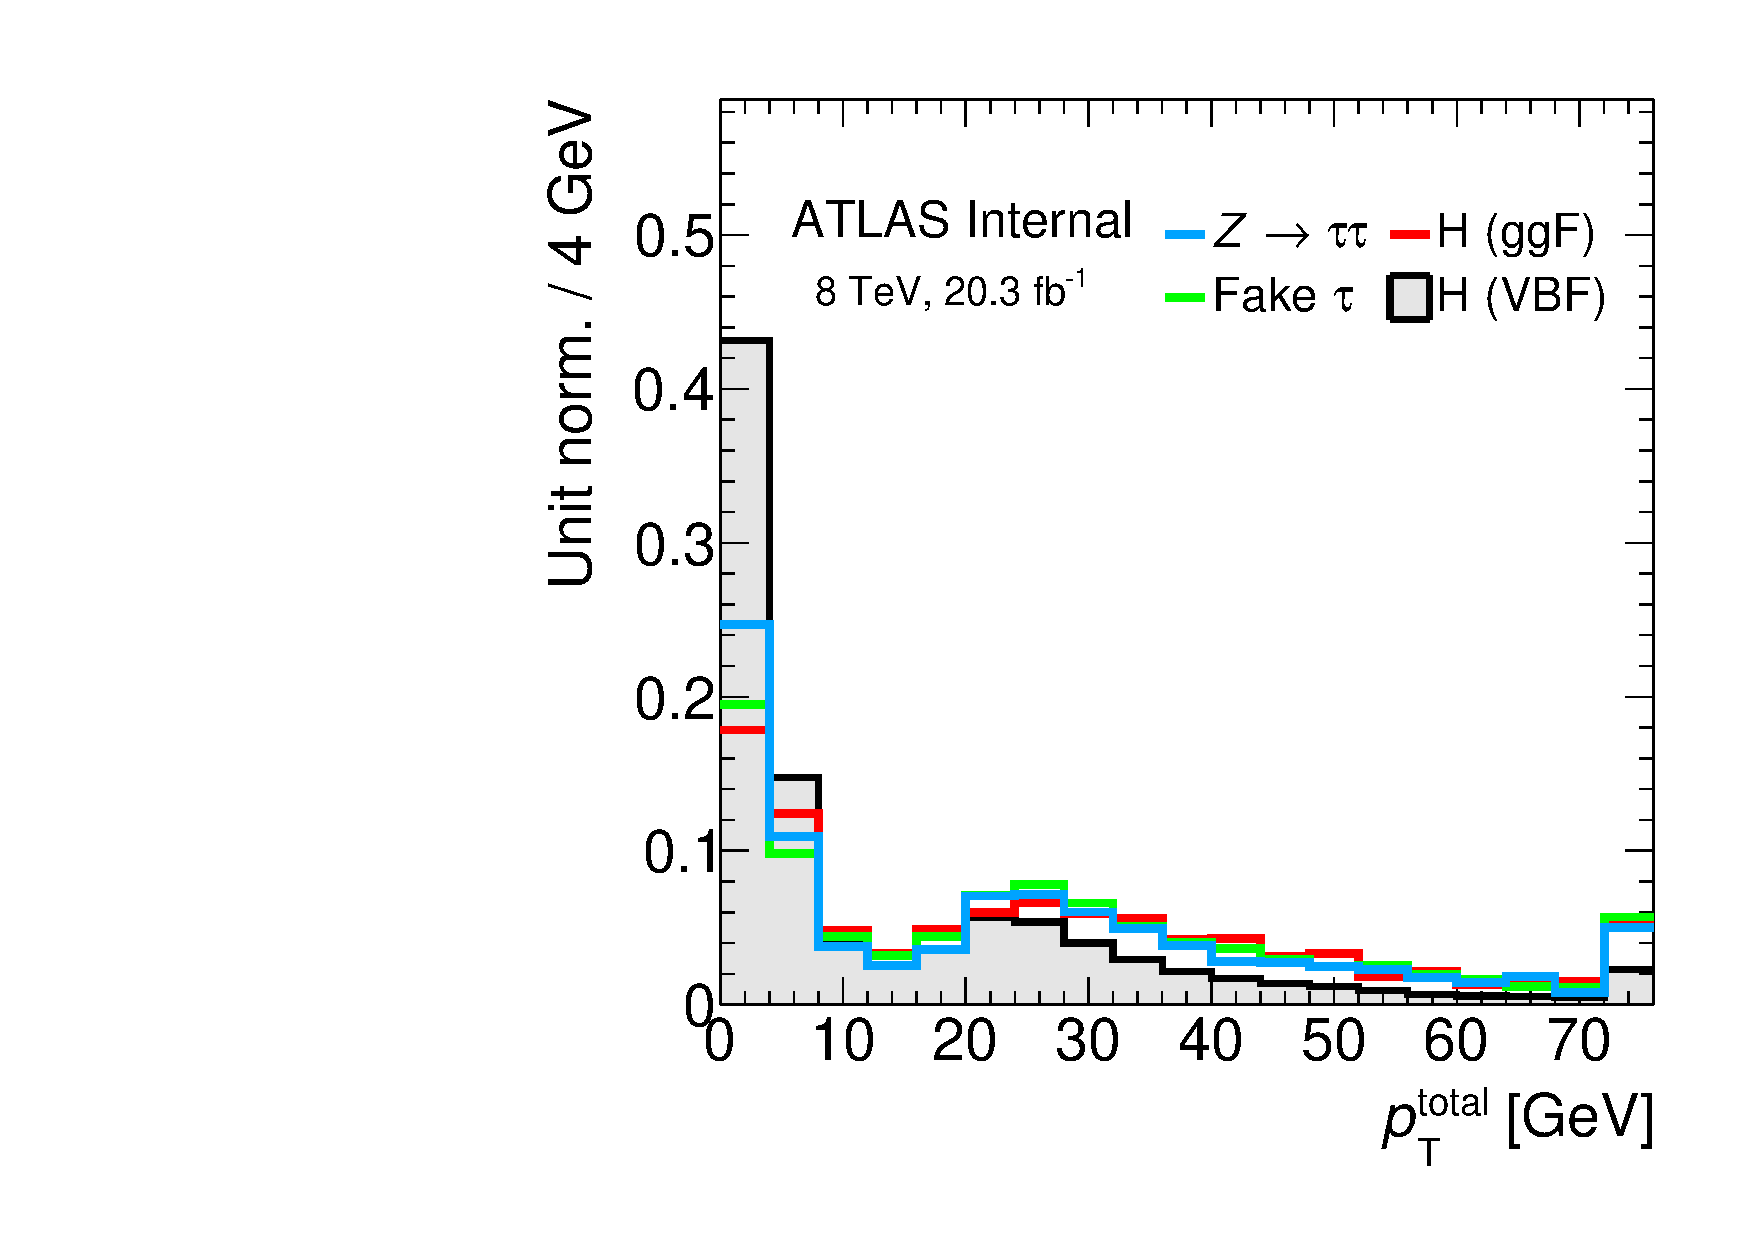
\includegraphics[width=0.45\textwidth]{figures/overlaid/vbf/system-pt}
  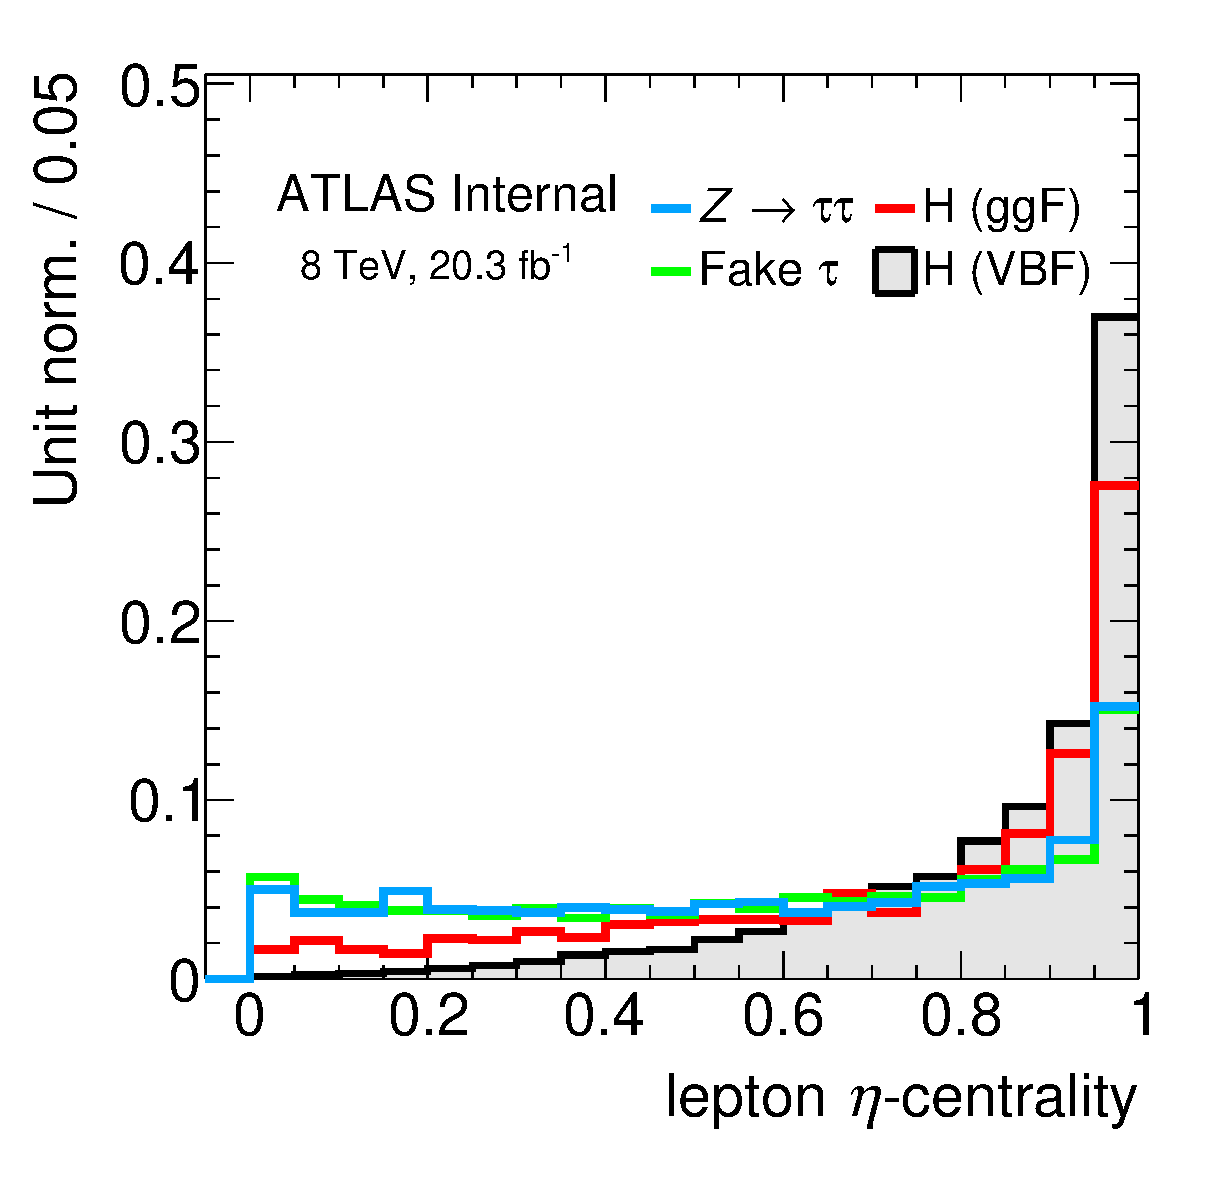
\includegraphics[width=0.45\textwidth]{figures/overlaid/vbf/lep-eta-centrality}
  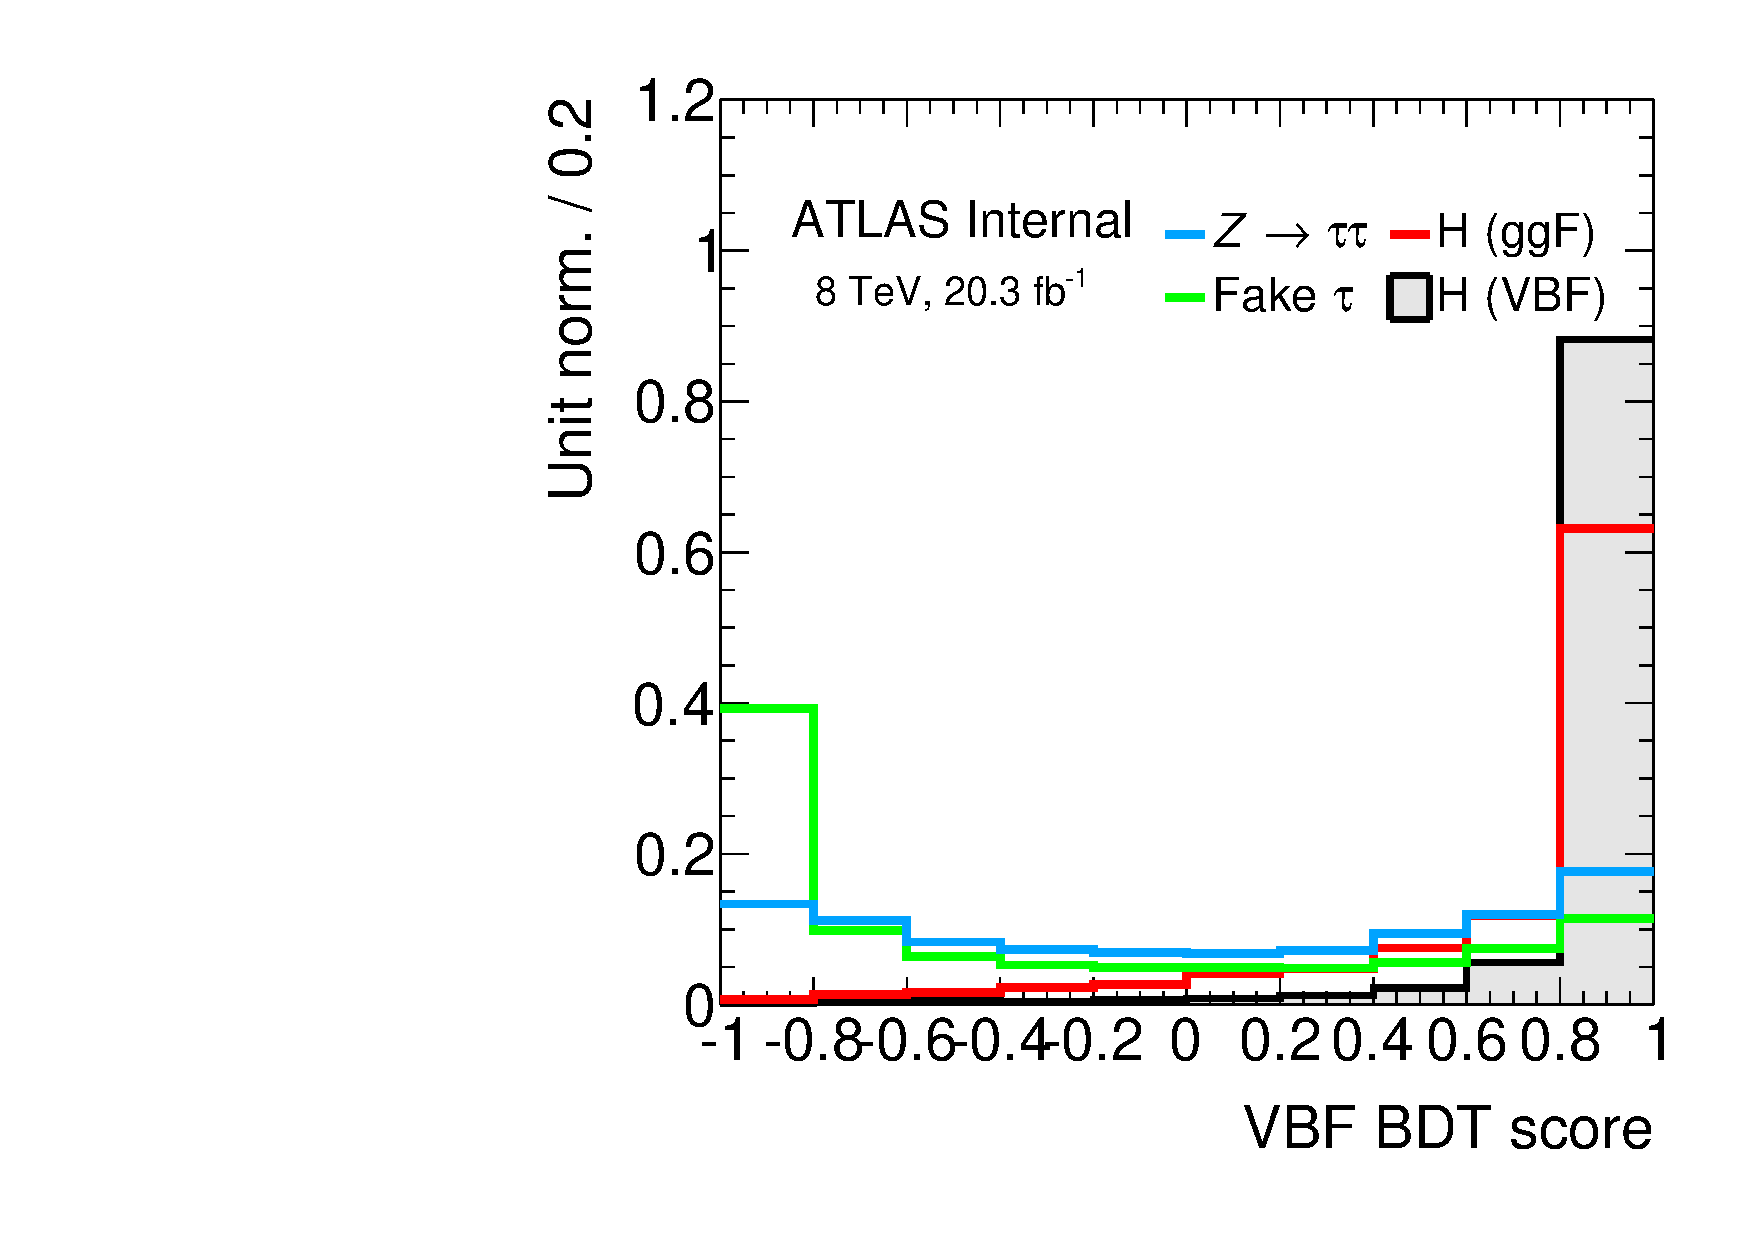
\includegraphics[width=0.45\textwidth]{figures/overlaid/vbf/BDTEve-VBF}
  \caption{Variables.}
  \label{fig:strategy-overlaid-vbf-other}
\end{figure}
% ---------------------------------------------------------------------------------

Here is a citation~\cite{1999.ATLAS.Physics-TDR}.


